%
%Не забыть:
%--------------------------------------
%Вставить колонтитулы, поменять название на титульнике



%--------------------------------------

\documentclass[a4paper, 12pt]{article} 

%--------------------------------------
%Russian-specific packages
%--------------------------------------
%\usepackage[warn]{mathtext}
\usepackage[T2A]{fontenc}
\usepackage[utf8]{inputenc}
\usepackage[english,russian]{babel}
\usepackage[intlimits]{amsmath}
\usepackage{esint}
%--------------------------------------
%Hyphenation rules
%--------------------------------------
\usepackage{hyphenat}
\hyphenation{ма-те-ма-ти-ка вос-ста-нав-ли-вать}
%--------------------------------------
%Packages
%--------------------------------------
\usepackage{amsmath}
\usepackage{amssymb}
\usepackage{amsfonts}
\usepackage{amsthm}
\usepackage{latexsym}
\usepackage{mathtools}
\usepackage{etoolbox}%Булевые операторы
\usepackage{extsizes}%Выставление произвольного шрифта в \documentclass
\usepackage{geometry}%Разметка листа
\usepackage{indentfirst}
\usepackage{wrapfig}%Создание обтекаемых текстом объектов
\usepackage{fancyhdr}%Создание колонтитулов
\usepackage{setspace}%Настройка интерлиньяжа
\usepackage{lastpage}%Вывод номера последней страницы в документе, \lastpage
\usepackage{soul}%Изменение параметров начертания
\usepackage{hyperref}%Две строчки с настройкой гиперссылок внутри получаеммого
\usepackage[usenames,dvipsnames,svgnames,table,rgb]{xcolor}% pdf-документа
\usepackage{multicol}%Позволяет писать текст в несколько колонок
\usepackage{cite}%Работа с библиографией
\usepackage{subfigure}% Человеческая вставка нескольких картинок
\usepackage{tikz}%Рисование рисунков
\usetikzlibrary{circuits} % подключаем библиотеки, содержащие
\usetikzlibrary{circuits.ee} % УГО для схем
\usetikzlibrary{circuits.ee.IEC}
\usetikzlibrary{arrows} % подключаем библиотеки со стрелками
\usetikzlibrary{patterns} % и со штриховкой
\usepackage{float}% Возможность ставить H в положениях картинки
% Для картинок Моти
\usepackage{misccorr}
\usepackage{lscape}
\usepackage{cmap}
\usepackage{bm}
\newtheorem{definition}{Опредление}



\usepackage{graphicx,xcolor}
\graphicspath{{Pictures/}}
\DeclareGraphicsExtensions{.pdf,.png,.jpg}

%----------------------------------------
%Список окружений
%----------------------------------------
\newenvironment {theor}[2]
{\smallskip \par \textbf{#1.} \textit{#2}  \par $\blacktriangleleft$}
{\flushright{$\blacktriangleright$} \medskip \par} %лемма/теорема с доказательством
\newenvironment {proofn}
{\par $\blacktriangleleft$}
{$\blacktriangleright$ \par} %доказательство
%----------------------------------------
%Список команд
%----------------------------------------
\newcommand{\grad}
{\mathop{\mathrm{grad}}\nolimits\,} %градиент

\newcommand{\diver}
{\mathop{\mathrm{div}}\nolimits\,} %дивергенция

\newcommand{\rot}
{\ensuremath{\mathrm{rot}}\,}

\newcommand{\Def}[1]
{\underline{\textbf{#1}}} %определение

\newcommand{\RN}[1]
{\MakeUppercase{\romannumeral #1}} %римские цифры

\newcommand {\theornp}[2]
{\textbf{#1.} \textit{ #2} \par} %Написание леммы/теоремы без доказательства

\newcommand{\qrq}
{\ensuremath{\quad \Rightarrow \quad}} %Человеческий знак следствия

\newcommand{\const}{\text{const}} % Написание const в формулах

\newcommand{\qlrq}
{\ensuremath{\quad \Leftrightarrow \quad}} %Человеческий знак равносильности

\renewcommand{\phi}{\varphi} %Нормальный знак фи

\renewcommand{\epsilon}{\varepsilon}

\newcommand{\me}
{\ensuremath{\mathbb{E}}}

\newcommand{\md}
{\ensuremath{\mathbb{D}}}



%\renewcommand{\vec}{\overline}




%----------------------------------------
%Разметка листа
%----------------------------------------
\geometry{top = 3cm}
\geometry{bottom = 2cm}
\geometry{left = 1.5cm}
\geometry{right = 1.5cm}
%----------------------------------------
%Колонтитулы
%----------------------------------------
\pagestyle{fancy}%Создание колонтитулов
\fancyhead{}
%\fancyfoot{}
\fancyhead[R]{\textsc{Экзамен. Оптика}}%Вставить колонтитул сюда
%----------------------------------------
%Интерлиньяж (расстояния между строчками)
%----------------------------------------
%\onehalfspacing -- интерлиньяж 1.5
%\doublespacing -- интерлиньяж 2
%----------------------------------------
%Настройка гиперссылок
%----------------------------------------
\hypersetup{				% Гиперссылки
	unicode=true,           % русские буквы в раздела PDF
	pdftitle={Заголовок},   % Заголовок
	pdfauthor={Автор},      % Автор
	pdfsubject={Тема},      % Тема
	pdfcreator={Создатель}, % Создатель
	pdfproducer={Производитель}, % Производитель
	pdfkeywords={keyword1} {key2} {key3}, % Ключевые слова
	colorlinks=true,       	% false: ссылки в рамках; true: цветные ссылки
	linkcolor=blue,          % внутренние ссылки
	citecolor=blue,        % на библиографию
	filecolor=magenta,      % на файлы
	urlcolor=cyan           % на URL
}
%----------------------------------------
%Работа с библиографией (как бич)
%----------------------------------------
\renewcommand{\refname}{Список литературы}%Изменение названия списка литературы для article
%\renewcommand{\bibname}{Список литературы}%Изменение названия списка литературы для book и report
%----------------------------------------
\begin{document}
	\begin{titlepage}
		\begin{center}
			$$$$
			$$$$
			$$$$
			$$$$
			{\Large{НАЦИОНАЛЬНЫЙ ИССЛЕДОВАТЕЛЬСКИЙ УНИВЕРСИТЕТ}}\\
			\vspace{0.1cm}
			{\Large{ВЫСШАЯ ШКОЛА ЭКОНОМИКИ}}\\
			\vspace{0.25cm}
			{\large{Факультет физики}}\\
			\vspace{5.5cm}
			{\Huge\textbf{{Экзамен}}}\\%Общее название
			\vspace{1cm}
			{\LARGE{<<Оптика>>}}\\%Точное название
			\vspace{2cm}
			\vfill
			\includegraphics[width = 0.2\textwidth]{HSElogo}\\
			\vfill
			Москва\\
			2020
		\end{center}
	\end{titlepage}
	
	\tableofcontents
	
	\newpage
	
	\section{Световой луч. Распространение световых лучей. Оптическая длина пути. Принцип Ферма, понятие таутохронима в оптике. Законы отражения и преломления света.}

\textbf{Световым лучом} мы будем называть некоторый конечный, но очень узкий пучок, который может существовать изолированно от других лучей.

Согласно \textbf{закону прямолинейного распространения света} световые лучи в прозрачной \textit{однородной} среде распространяются прямолинейно. Согласно \textbf{закону о независимости световых пучков} распространение каждого светового луча не зависит от того, есть ли в среде иные световые лучи, или нет. Это разумеется, не совсем корректно: тогда бы не было явления интерференции, однако в рамках геометрической оптики мы этим явлением пренебрежем.

\textbf{Оптической длиной пути} $\Delta$ между двумя точками мы назовем расстояние, на которое свет распространился бы в вакууме за время прохождения расстояния между этими двумя точками. Как известно, скорость света в вакууме есть максимальная достижимая скорость и является константой $c$, а скорость света в веществе равна:

\begin{equation}
v = \frac{c}{n}
\label{eq:n_introduct}
\end{equation}

где $n$ --- абсолютный показатель преломления среды, который и вводится, как отношение скорости света в вакууме к скорости света в этой среде.

Тогда на основании формулы (\ref{eq:n_introduct}) можем записать:

\begin{equation*}
\Delta = n l
\end{equation*} 

где $l$ --- расстояние между точками, $n$ --- абсолютный показатель преломления среды.

Указанная формула имеет обобщение на случай, когда показатель среды может зависеть от координаты, тогда:

\begin{equation}
\Delta = \int\limits_a^b n dl
\label{eq:delta_introduct}
\end{equation} 

\theornp{Принцип Ферма}{Луч движется из начальной точки в конечную по траектории, которая обеспечивает минимальную оптическую длину пути. Является \textbf{постулатом}.} 

Из принципа Ферма в случае однородной среды логичным образом вытекает закон прямолинейного распространения света, упомянутый ранее.

\theornp{Принцип таутохронизма}{Оптическая длина любого луча между двумя волновыми фронтами одна и та же.}

\theornp{Закон отражения света}{Луч падающий, луч отраженный и перпендикуляр, восстановленный из точки падения, лежат в одной полуплоскости. Угол падения равен углу отражения.}

\begin{theor}{Закон преломления света}{Луч падающий, луч преломленный и перпендикуляр, восстановленный в точке преломления, лежат в одной плоскости. Угол падения и угол преломления связаны следующим соотношением: $n_{1} \sin \alpha = n_{2} \sin \gamma$, где $n_1$ --- абсолютный показатель преломления среды, из которой луч приходит, $n_2$ --- среды, в которую луч преломляется, $\alpha$ --- угол падения, $\gamma$ --- угол преломления.}
	Пусть глаз наблюдателя находится на высоте H над поверхностью некоего водоема, а точечный источник --- на глубине $h$ в этом водоеме на расстоянии $S$ от места, где стоит наблюдатель (вдоль поверхности воды). Показатель преломления воздуха примем равным $n_{\text{возд}} = 1$, а показатель преломления воды --- $n$, известный нам.
	
	Пусть проекция отреза $BS$ на поверхность воды равна $x$. В таком случае:
	
	\begin{align*}
	BS&=\sqrt{h^{2}+x^{2}},\\
	MB&=\sqrt{H^{2}+(L-x)^{2}} \\ 
	t=\frac{SB}{v}+\frac{MB}{c}&=\left(n_{1}\sqrt{h^{2}+x^{2}}+\sqrt{H^{2}+(L-x)^{2}}\right) / c
	\end{align*}
	
	Согласно принципу наименьшего времени, полученное нами последнее выражение должно оказаться минимальным, другими словами $\dfrac{dt}{dx} = 0$ или:
	
	\begin{equation*}
	n_{1} \frac{x}{\sqrt{h^{2}+x^{2}}}-\frac{L-x}{\sqrt{H^{2}+(L-x)^{2}}}=0
	\end{equation*}
	
	\begin{figure}[H]
		\centering
		\includegraphics*[width=0.5\textwidth]{Snellius}
	\end{figure}
	
	В то же время из рисунка мы однозначно можем утверждать:
	
	\begin{align*}
	\sin \alpha &= \frac{x}{\sqrt{h^{2}+x^{2}}}\\
	\sin \gamma &= \frac{L-x}{\sqrt{H^{2}+(L-x)^{2}}}
	\end{align*}
	
	
	
	Отсюда напрямую следует факт:
	
	\begin{equation*}
	\boxed{n\sin\alpha = \sin\gamma}
	\end{equation*}
	
\end{theor}
	
	\newpage
	
	\input{TeX_files/2.tex}
	
	\newpage
	
	\input{TeX_files/3.tex}
	
	\newpage
	
	
\section{Построение изображений. Центрированная оптическая система. Кардинальные точки и плоскости центрированной оптической системы. Сложение центрированных оптических систем. Отражение от сферических поверхностей. Фокусное расстояние выпуклого и вогнутого зеркал. Схема построения изображений для зеркал.}



\subsection{Основные определения}

\textit{Оптическая ось оптической системы} (включаюзая линзы, зеркала и так далее) - прямая линия, являющаяся осью симметрии преломляющих (отражающих) поверхностей. Она проходит перпендикулярно этим поверхностям через центры их кривизны.

\medskip

\textit{Центрированная оптическая система} - совокурность однородных преломляющих и отражающих сред, отдаленных друг от друга симметричными поверхностями, центры кривизны которых находятся на одной прямой. Эту прямую называют \textit{главной оптической осью}.

\medskip

Две сопряженные плоскости, отображающиеся с линейным увеличением +1, называются \textit{главными}. Одна из них называется главной плоскотью пространства предметов (или передней главной плоскостью), а вторая - главной плоскостью пространства изображений (или задней главной плоскостью).  Точки пересечения главных плоскостей с главной оптической осью называются главными точками оптической системы.

Фокальные и главные точки центрированной системы называются ее \textit{кардинальными точками}.

\subsection{Построений изображений}

Знание кардинальных точек позволяет строить изображение произвольного предмета. Для этого из точек предмета проводят два луча: один - параллельно главной оптической оси, а второй - через передний фокус. Первый луч, достигнув главной плоскости, преобразуется в луч, идущий через задний фокус, а второй - в луч, идущий параллельно оптической оси. Точка пересечения вторичных лучей (или их продолжений в обратном направлении) дает изображение (действительное или мнимое) соответствующих точек предмета.

\subsection{Сложение центрированных оптических систем}

\subsubsection{Фокусные расстояния составной системы}

Рассмотрим две центрированные системы, главные оптические оси которых совпадают. Составная система при этом также оказывается центрированной.

Расстояние $\Delta$ между задним фокусом $F'_1$ первой системы и передним фокусом $F_2$ второй называется \textit{оптическим интервалом} двух складываемых систем.

\bigskip

Будем решать задачу о нахождении фокусных расстояний сложной системы, зная фокусные расстояния складываемых систем и оптический интервал между ними. Будем считать, что пространство между главными плоскостями $H_1'$ и $H_2$ складываемых оптических систем однородно и имеет показатель преломления $n$.

\medskip

\begin{figure}[h!]
    \centering
    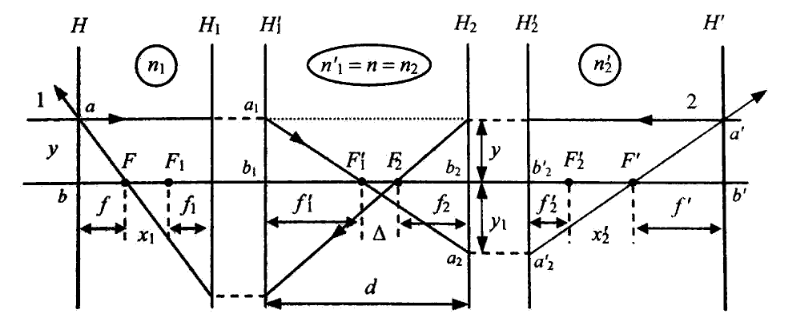
\includegraphics[scale=1]{kartin_ochka.png}
    \label{fig:my_label}
\end{figure} 


Пошлем луч 1 слева направо параллельно главной оптической оси. Данный луч пройдет на расстоянии $\Delta$ от переднего фокуса $F_2$ системы 2 и пересечет главную оптическую ось в точке $F'$, являющейся задним фокусом составной системы. Это позволяет найти расстояние $x_2'$ от заднего фокуса $F_2'$ системы 2 до заднего фокуса $F'$ составной системы. По формуле Ньютона(получается из геометрии треугольников) после прохождения второй системы имеем 

\begin{equation*}
    (-\Delta)\cdot x_2^{'} = f_2 f_2^{'} \Rightarrow x_2^{'} = -\frac{f_2f_2^{'}}{\Delta}
\end{equation*}


Для нахождения фокусного расстояния $f^{'}$ нужно найти положение главной плоскости $H^{'}$ составной системы. Из подобия треугольников $a_1b_1F_1^{'}$ и $a_2b_2F_1^{'}$ следует равенство

\begin{equation*}
    \frac{y}{-y^{'}} = \frac{f_1^{'}}{\Delta - f_2}
\end{equation*}

Для прямоугольных треугольников $a^{'}b^{'}F^{'}$ и $a_2^{'}b_2^{'}F^{'}$

\begin{equation*}
    \frac{y}{-y^{'}} = \frac{-f^{'}}{f_2^{'} +x_2^{'}}
\end{equation*}

Подстановка сюда выражения $x_2^{'} = -\frac{f_2f^{'}}{\Delta}$ дает

\begin{equation*}
    \frac{y}{-y_1} = \frac{f^{'}}{f_2^{'} - \frac{f_2f_2^{'}}{\Delta}} = -\frac{f^{'}\Delta}{f_2^{'}(\Delta-f_2)}
\end{equation*}


Сравнив полученные выражения, получим итоговую формулу для заднего фокусного расстояния $f^{'}$:

\begin{equation*}
    f^{'} = -\frac{f_1^{'}f_2^{'}}{\Delta}
\end{equation*}

Положение передней главной плоскости и переднее фокусное расстояние можно найти, есои рассмотреть траекторию луча 2, запущенного в обратном направлении. Проводя аналогичные рассуждения, получим расстояние от переднего фокуса $F_1$ системы 1 до переднего фокуса $F$ составной системы и суммарное переднее фокусное расстояние:

\begin{equation*}
    x_1 = \frac{f_1f_1^{'}}{\Delta}, \hspace{10px} f=\frac{f_1f_2}{\Delta}
\end{equation*}
\subsubsection{Оптическая сила составной системы}

После преобразований полученного выражения для фокуса с помощью определения оптической силы, получим

\begin{equation*}
    \Phi = \Phi_1 + \Phi_2 -\frac{d}{n}\Phi_1\Phi_2.
\end{equation*}

В частном случае, когда $d \rightarrow 0$, получаем, что оптическая сила сложной системы равна сумме оптических сил составляющих систем:
\begin{equation*}
    \Phi = \Phi_1 + \Phi_2.
\end{equation*}

Этот результат можно распространить на случай произвольного числа элементов составной оптической системы, если только эти элементы расположены достаточно близко:

\begin{equation*}
    \Phi = \sum_i \Phi_i.
\end{equation*}

\subsection{Отражение от сферических поверхностей. Фокусное расстояние выпуклого и вогнутого зеркал}



Запишем выражение для оптической силы преломляющей поверхности:

\begin{equation*}
    \Phi = -\frac{n-n^{'}}{R}
\end{equation*}

Знание оптической силы позволяет найти фокуное расстояние:

\begin{equation*}
    f^{'} = \frac{n^{'}}{\Phi}
\end{equation*}

Для зеркала оптическая сила может быть определена, если положить $n = 1, n^{'} = -1$

\begin{equation*}
    \Phi = -\frac{2}{R}
\end{equation*}

Для выпуклого зеркала $R > 0, \Phi < 0$. Это зеркало будет рассеивать падающее на него излучение. Если же $R < 0$, то зеркало фокусирует излучение $(\Phi > 0)$.

\begin{figure}[h!]
    \centering
    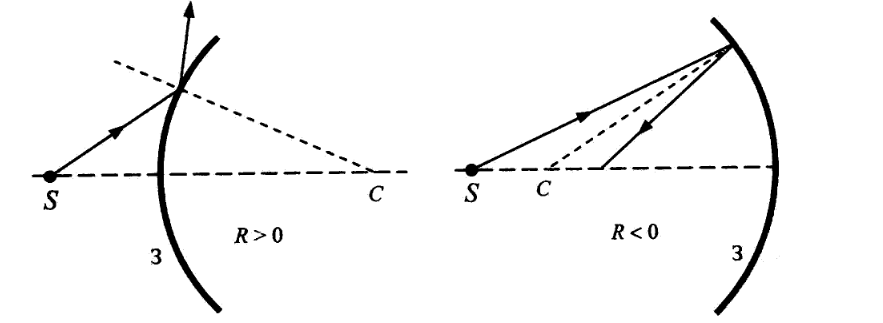
\includegraphics[scale=0.8]{mirror.png}
    \caption{Слева - отражение выпуклым зеркалом; справа - отражение вогнутым }
    \label{fig:my_label}
\end{figure} 

\subsection{Схема построения изображений для зеркал}


\subsubsection{Построение изображения в плоском зеркале}

Общие идеи:

\begin{enumerate}
    \item Падающий на зеркало луч, отражается, согласно закону отражения
    \item Изображение строится на пересечении продолжения падающих лучей за плоскость зеркала
    \item Предмет и изображение расположены симметрично относительно плоскости зеркала
    \item Изображение мнимое
\end{enumerate}

\subsubsection{Построение изображения в сферическом зеркале}
Общие идеи построения изображения в сферическом зеркале совпадают с принципами построения изображения в линзах: 

\begin{enumerate}
    \item Луч, пущенный вдоль главной оптической оси, после отражения пойдет через фокус
    \item Луч, проходящий через фокус, отразившись, окажется параллельным ГОО
    \item Луч, проходящий через центр кривизны зеркала, после отражения пройдет по тому же пути
    \item Изображение строится на пересечении лучей или их продолжений
\end{enumerate}

	
	\newpage
	
	\section{Аберрации оптических систем. Аберрации, обусловленные широкими пучками лучей. Коррекция сферической и хроматической аберрации.}
	\subsection{Аберрации оптических систем.}
	\begin{definition}
		\textbf{Аберрации оптических систем} (лат. aberratio - уклонение),
		погрешности изображений, даваемых оптическими системами.
		Проявляются в том, что оптические изображения в ряде случаев не
		вполне отчётливы, не точно соответствуют объекту или оказываются
		окрашенными.
	\end{definition}
	Аберации делят на \textbf{\textit{монохроматические (геометрические)}} и \textbf{\textit{хроматические}}, среди геометрических ывделяют
	\begin{itemize}
		\item Сферическая аберрация
		\item Кома
		\item Астигматизм
		\item Дисторсия 
		\item Кривизна поля (поверхности) изображения
	\end{itemize}
	\subsubsection{Классификация геометрических аберраций}
	Геометрические аберрации практичеки всегда являются учётом непараксиальности в ходе лучей. Произвольный луч в пространстве можно задать, указав прямоугольные координаты $y$, $z$, $\eta$ и $\zeta$ точек его пересечения с  предметной плоскостью (т.е. плоскостью, проходящей через изображаемую точку $P$ перпендикулярно к главной оптической оси) и плоскостью входного зрачка. После прохождения через оптическую систему луч пересечёт плоскость параксиального изображения в точке с координатами $y'$ и $z'$. Координаты самого параксиального изображения (\textit{параксиального фокуса}) -- $y_{0}'$, $z'_{0}$. Разности
	\begin{align*}
	\Delta y' &= y' - y'_{0} & \Delta z' &= z'- z'_{0}
	\end{align*} 
	примем за меру отступления от предельного случая параксиальной оптики.
	Координаты $y'$  и  $z'$ будут функциями $y$, $z$, $\eta$ и $\zeta$:
	\begin{align*}
	y' &= f_{y}(y,z,\eta,\zeta) & z' &= f_{z}(y,z,\eta,\zeta)
	\end{align*}
	Линейные члены разложений $f_{y}$ и $f_{z}$ не зависят от $\eta$ и $\zeta$ и соответствуют параксиальной оптике, члены чётных степеней не войдут в эти разложения в силу осевой симметрии оптической задачи. Поэтому $\Delta y'$ и $\Delta z'$ будут определятся третьими членами разложения $f_{y}$ и $f_{z}$ (пожтому часто рассматриваемые дальше аберрации называются аберрациями третьего порядка).
	 
	Введём три вектора, перпендикулярных главной оптической оси системы:
	\begin{align*}
	\mathbf{r} &= y\mathbf{j} + z\mathbf{k} & \mathbf{r}' &= y'\mathbf{j} + z'\mathbf{k} & \bm{\sigma} &= \eta\mathbf{j} + \zeta\mathbf{k}
	\end{align*}
	Тогда вектор 
	\begin{equation*}
	\Delta \mathbf{r}' = \Delta y'\mathbf{j} + \Delta z'\mathbf{k}
	\end{equation*}
	может быть разложен по векторам $\mathbf{r}$ и $\bm{\sigma}$.
 	Причём в виду симметрии коэффициенты этих разложения могут зависеть только от <<инвариантов вращения>> $\bm{\sigma}^{2}$, $(\bm{\sigma}\mathbf{r})$ и $r^{2}$:
 	\begin{equation}
 	\label{series3}
 	\Delta \mathbf{r}' \approx \Big(A\bm{\sigma}^{2} + B(\bm{\sigma}\mathbf{r}) + C\mathbf{r}^{2}\Big)\bm{\sigma} + \Big(D\bm{\sigma}^{2} + E(\bm{\sigma}\mathbf{r}) + F\mathbf{r}^{2}\Big)\mathbf{r}
 	\end{equation}
 	В дальнейшем под $|\bm{\sigma}|$ понимается радиус входного зрачка. \textit{Аберрационной} кривой называют кривую, по которой плоскость параксиального изображения пересекает пучок лучей, проведённых из точки-объекта $P$ через окружность входного зрачка. Изображением вместо точки теперь окажется область, ограниченная аберрационной кривой.
 	
 	Каждый из постоянных коэффициентов $A$, $B$, $C$, $D$, $E$ и $F$ в уравнении (\ref{series3}) определяется конфигурацией оптической системы и отвечает за конкретный тип аберрации. Аберрация определяемая членом $A\bm{\sigma}^{2}\bm{\sigma}$ называется \color{blue}{сферической}\normalcolor. Членам $B(\bm{\sigma}\mathbf{r})\bm{\sigma} + D\bm{\sigma}^{2}\mathbf{r}$ соответствует \color{blue}{кома}\normalcolor. Членам $C\mathbf{r}^{2}\bm{\sigma} + E(\bm{\sigma} r)\mathbf{r}$ -- \color{blue}{астигматизм косых лучей} \normalcolor и \color{blue}{искривление плоскости изображения}\normalcolor. Члену $F\mathbf{r}^{2}\mathbf{r}$  соответствует \color{blue}{дисторсия}\normalcolor.
 	\subsubsection{Сферическая аберрация}
 	\begin{figure}[H]
 	\begin{center}
 	\includegraphics[scale=0.36]{5_sferober.png}
 	\caption{Схема сферической аберрации, где
 		$H$, $H'$ — положения главных плоскостей;
 		$F'$  — задняя фокальная плоскость;
 		$f'$  — заднее фокусное расстояние;
 		$-\delta s'$  — продольная сферическая аберрация;
 		$\delta g' = \Delta r'$  — поперечная сферическая аберрация.}
 	\label{p1}
 	\end{center}
 	\end{figure}
 \begin{definition}
 	\textbf{Сферическая аберрация} — аберрация оптических систем из-за несовпадения фокусов для лучей света, проходящих на разных расстояниях от оптической оси (см. рис.~\ref{p1}.).
 \end{definition}
Так как сферическая аберрация отвечает члену $A\bm{\sigma}^{2}\bm{\sigma}$, то если в системе есть только этот тип аберрации ($|B|,|C|,|D|,|E|,|F|\approx0\ll |A|$), то
\begin{equation*}
|\Delta r'| = A\sigma^{3} = const
\end{equation*} 
а значит аберрационной окривой является окружность (радиус которой пропорционален кубу входного зрачка), а изображение -- круглое пятнышко, ограниченное этой окружностью (см. рис.~\ref{p1}).

\begin{wrapfigure}{r}{0.5\textwidth}
	\begin{tikzpicture}
	\draw (-2.598,-1.5) arc (210:150:3);
	\draw (-2.598,1.5) -- (0,0);
	\draw (-2.598,-1.5) -- (0,0);
	\draw (-2.598,1.5) -- (0,0);
	\draw (-2.598,-1.5) -- (0,0);
	\draw (-2.704,1.3) -- (0.2,0);
	\draw (-2.704,-1.3) -- (0.2,0);
	\draw (-2.791,1.1) -- (0.4,0);
	\draw (-2.791,-1.1) -- (0.4,0);
	\draw (-2.862,0.9) -- (0.6,0);
	\draw (-2.862,-0.9) -- (0.6,0);
	\draw (-2.917,0.7) -- (0.8,0);
	\draw (-2.917,-0.7) -- (0.8,0);
	\draw (-2.958,0.5) -- (1.0,0);
	\draw (-2.958,-0.5) -- (1.0,0);
	\draw (-2.985,0.3) -- (1.2,0);
	\draw (-2.985,-0.3) -- (1.2,0);
	\draw (-2.998,0.1) -- (1.4,0);
	\draw (-2.998,-0.1) -- (1.4,0);
	\end{tikzpicture}
	\caption{Каустика -- огибающая лучей от фронта}
	\label{kau}
\end{wrapfigure}
В результате сферической аберрации цилиндрический пучок лучей, после преломления линзой (в пространстве изображений) получает вид не конуса, а некоторой воронкообразной фигуры, наружная поверхность которой, вблизи узкого места, называется каустической поверхностью (см. рис.~\ref{kau}). При этом изображение точки имеет вид диска с неоднородным распределением освещённости, а форма каустической кривой позволяет судить о характере распределения освещённости. В общем случае, фигура рассеяния, при наличии сферической аберрации, представляет собой систему концентрических окружностей с радиусами пропорциональными третьей степени координат на входном (или выходном) зрачке.

\begin{wrapfigure}{r}{0.55\textwidth}
	\begin{tikzpicture}[>=latex']
	\draw[black] (-2.598,-1.5) arc (210:150:3);
	\draw[black] (-2.4,-1.5) arc (-30:30:3);
	\draw[black] (-2.4,-1.5) -- (-2.598,-1.5); 
	\draw[black] (-2.4,1.5) -- (-2.598,1.5);
	\draw[black,->] (-4,-1.2) -- (-3,-1.2);
	\draw[black] (-4,-1.2) -- (-2.75,-1.2);
	\draw[black,->] (-4,1.2) -- (-3,1.2);
	\draw[black] (-4,1.2) -- (-2.75,1.2);
	\draw[red,->] (-2.75,1.2) -- (-2.22,1.15);
	\draw[green,->] (-2.75,1.2) -- (-2.2,1.1);
	\draw[blue,->] (-2.75,1.2) -- (-2.18,1.05);
	\draw[red,->] (-2.75,-1.2) -- (-2.22,-1.15);
	\draw[green,->] (-2.75,-1.2) -- (-2.2,-1.1);
	\draw[blue,->] (-2.75,-1.2) -- (-2.18,-1.05);
	\draw[red] (-2.22,1.15) -- (2,0);
	\draw[green] (-2.2,1.1) -- (1.5,0);
	\draw[blue] (-2.18,1.05) -- (1,0);
	\draw[red] (-2.22,-1.15) -- (2,0);
	\draw[green] (-2.2,-1.1) -- (1.5,0);
	\draw[blue] (-2.18,-1.05) -- (1,0);
	\draw[red,->] (-2.22,1.15) -- (-0.11,0.575);
	\draw[green,->] (-2.2,1.1) -- (-0.35,0.55);
	\draw[blue,->] (-2.18,1.05) -- (-0.59,0.525);
	\draw[red,->] (-2.22,-1.15) -- (-0.11,-0.575);
	\draw[green,->] (-2.2,-1.1) -- (-0.35,-0.55);
	\draw[blue,->] (-2.18,-1.05) -- (-0.59,-0.525);
	\draw[gray,dashdotted] (-4,0)--(2.5,0);
	\end{tikzpicture}
	\caption{Пример хроматической аберрации.}
	\label{p3}
\end{wrapfigure} 

Сферическая аберрация линзы (системы линз) объясняется тем, что её преломляющие поверхности встречают отдельные лучи сколько-нибудь широкого пучка под различными углами. Вследствие чего, более удалённые от оптической оси лучи преломляются сильнее, нежели нулевые лучи, и образуют свои точки схода удалённые от фокальной плоскости.
\subsubsection{Хроматическая аберрация}
Если используется белый свет, то в изображении возникают дополнительные аберрации. Это связано с тем, что показатель прломления зависит от длины волны (дисперсия света). Поэтому оптическая сиситема даёт не одно, а множнство монохроматических изображений, отличающихся друг от друга по величине и положению. Результирующее же изображение, получающееся от нложения таких монохроматических изображений, оказывается нерезким и с окрашенными краями. Это явление и называется \textit{хроматической аберрацией} (например рис.~\ref{p3}).
\subsection{Аберрации, обусловленные широкими пучками лучей.}
К аберрациям, обусловленные широкими пучками лучей из монохроматическим относят сферическую аберрацию и кому. (Сферическую оберацию смотри выше).
\begin{wrapfigure}{l}{0.55\textwidth}
	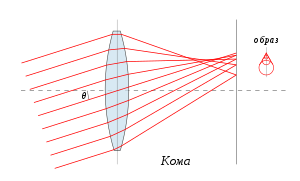
\includegraphics[scale=0.7]{5_coma.png}
	\caption{Коматическая аберрация или кома.}
	\label{coma}
\end{wrapfigure}
\subsubsection{Кома}
Каждый участок оптической системы, удалённый от её оси на расстояние $d$ (кольцевая зона), даёт изображение светящейся точки в виде кольца, радиус которого тем больше, чем больше $d$; может рассматриваться как сферическая аберрация лучей, проходящих не через оптическую ось системы. Центры колец не совпадают, в результате чего их наложение, то есть изображение точки, даваемое системой в целом, принимает вид несимметричного пятна рассеяния, похожего на комету. Этим сходством и обусловлено название аберрации (см. рис.~\ref{coma}). Размеры пятна пропорциональны квадрату угловой апертуры системы и удалению точки-объекта от оси оптической системы. 
\subsection{Коррекция сферической и хроматической аберрации.}
И сферическая и хроматическая аберрации могут быть с той или иной мерой точности откорректированы путём комбинации линз (например, рис.~\ref{p4gl}).
\begin{figure}[H]
	\begin{center}
	\subfigure{\label{p40}}
	\begin{tikzpicture}[>=latex']
	\draw[black] (-2.598,-1.5) arc (210:150:3);
	\draw[black] (-2.4,-1.5) arc (-30:30:3);
	\draw[black] (-2.4,-1.5) -- (-2.598,-1.5); 
	\draw[black] (-2.4,1.5) -- (-2.598,1.5);
	\draw[black,->] (-4,-1.2) -- (-3,-1.2);
	\draw[black] (-4,-1.2) -- (-2.75,-1.2);
	\draw[black,->] (-4,1.2) -- (-3,1.2);
	\draw[black] (-4,1.2) -- (-2.75,1.2);
	\draw[red,->] (-2.75,1.2) -- (-2.22,1.15);
	\draw[green,->] (-2.75,1.2) -- (-2.2,1.1);
	\draw[blue,->] (-2.75,1.2) -- (-2.18,1.05);
	\draw[red,->] (-2.75,-1.2) -- (-2.22,-1.15);
	\draw[green,->] (-2.75,-1.2) -- (-2.2,-1.1);
	\draw[blue,->] (-2.75,-1.2) -- (-2.18,-1.05);
	\draw[red] (-2.22,1.15) -- (2,0);
	\draw[green] (-2.2,1.1) -- (1.5,0);
	\draw[blue] (-2.18,1.05) -- (1,0);
	\draw[red] (-2.22,-1.15) -- (2,0);
	\draw[green] (-2.2,-1.1) -- (1.5,0);
	\draw[blue] (-2.18,-1.05) -- (1,0);
	\draw[red,->] (-2.22,1.15) -- (-0.11,0.575);
	\draw[green,->] (-2.2,1.1) -- (-0.35,0.55);
	\draw[blue,->] (-2.18,1.05) -- (-0.59,0.525);
	\draw[red,->] (-2.22,-1.15) -- (-0.11,-0.575);
	\draw[green,->] (-2.2,-1.1) -- (-0.35,-0.55);
	\draw[blue,->] (-2.18,-1.05) -- (-0.59,-0.525);
	\draw[gray,dashdotted] (-4,0)--(2.5,0);
	\end{tikzpicture}
	\subfigure{\label{p4}}
	\begin{tikzpicture}[>=latex']
	\draw[black] (-2.598,-1.5) arc (210:150:3);
	\draw[black,thick] (-2.4,-1.5) arc (-30:30:3);
	\draw[black] (-2.4,-1.5) -- (-2.598,-1.5); 
	\draw[black] (-2.4,1.5) -- (-2.598,1.5);
	\draw[black,->] (-4,-1.2) -- (-3,-1.2);
	\draw[black] (-4,-1.2) -- (-2.75,-1.2);
	\draw[black,->] (-4,1.2) -- (-3,1.2);
	\draw[black] (-4,1.2) -- (-2.75,1.2);
	\draw[red,->] (-2.75,1.2) -- (-2.22,1.15);
	\draw[green,->] (-2.75,1.2) -- (-2.2,1.1);
	\draw[blue,->] (-2.75,1.2) -- (-2.18,1.05);
	\draw[red,->] (-2.75,-1.2) -- (-2.22,-1.15);
	\draw[green,->] (-2.75,-1.2) -- (-2.2,-1.1);
	\draw[blue,->] (-2.75,-1.2) -- (-2.18,-1.05);
	\draw[black] (-2.4,1.5) -- (-1.6,1.5) -- (-1.6,-1.5) -- (-2.4,-1.5);
	\draw[gray,dashdotted] (-4,0)--(2.5,0);
	%
	\draw[red,->] (-2.22,1.15) -- (-1.6,1.075);
	\draw[green,->] (-2.2,1.1) -- (-1.6,1.05);
	\draw[blue,->] (-2.18,1.05) -- (-1.6,1.03);
	\draw[red,->] (-2.22,-1.15) -- (-1.6,-1.075);
	\draw[green,->] (-2.2,-1.1) -- (-1.6,-1.05);
	\draw[blue,->] (-2.18,-1.05) -- (-1.6,-1.03);
	%
	\draw[red] (-1.6,1.075) -- (2.5,0);
	\draw[green] (-1.6,1.05) -- (2.3,0);
	\draw[blue] (-1.6,1.03) -- (2.1,0);
	\draw[red] (-1.6,-1.075) -- (2.5,0);
	\draw[green] (-1.6,-1.05) -- (2.3,0);
	\draw[blue] (-1.6,-1.03) -- (2.1,0);
	\draw[red,->] (-1.6,1.075) -- (0.45,0.5375);
	\draw[green,->] (-1.6,1.05) -- (0.35,0.525);
	\draw[blue,->] (-1.6,1.03) -- (0.25,0.515);
	\draw[red,->] (-1.6,-1.075) -- (0.45,-0.5375);
	\draw[green,->] (-1.6,-1.05) -- (0.35,-0.525);
	\draw[blue,->] (-1.6,-1.03) -- (0.25,-0.515);
	\end{tikzpicture}
	\end{center}
	\caption{Пример коррекции хроматической аберрации на собирающеё линзе при помощи рассеивающей линзы. Аналогичным образом можно корректировать и сферические аберрации.}
	\label{p4gl}
\end{figure}
На рисунке~\ref{korwiki} представлены способы коррекции сферической аберрации при помощью дифрагмирования и расфокусировки линзы. 
\begin{figure}[H]
	\centering
	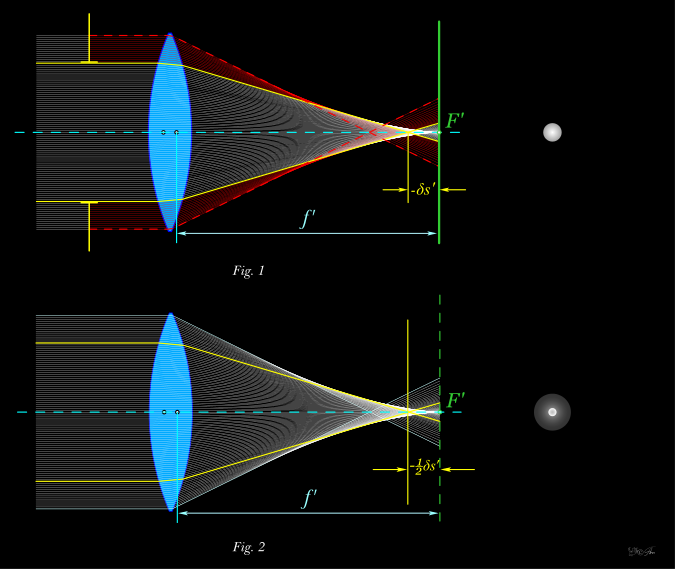
\includegraphics[scale=0.45]{5_sfer_kor.png}
	\caption{Коррекция сферической аберрации: наверху -- при помощи дифрагмирования, снизу --  при помощи расфокусировки.}
	\label{korwiki}
\end{figure} 
Заметное влияние на сферическую аберрацию оказывает диафрагмирование объектива (или иной оптической системы), так как при этом отсекаются краевые лучи широкого пучка. Очевидно, что этот способ непригоден для оптических систем, требующих высокой светосилы. 

В отдельных случаях небольшая величина сферической аберрации третьего порядка может быть исправлена за счёт некоторой дефокусировки объектива. При этом плоскость изображения смещается к, так называемой, «плоскости лучшей установки», находящейся, как правило, посередине, между пересечением осевых и крайних лучей, и не совпадающей с самым узким местом пересечения всех лучей широкого пучка (диском наименьшего рассеяния). Это несовпадение объясняется распределением световой энергии в диске наименьшего рассеяния, образующей максимумы освещённости не только в центре, но и на краю. То есть, можно сказать, что «диск» представляет из себя яркое кольцо с центральной точкой. Поэтому, разрешение оптической системы, в плоскости совпадающей с диском наименьшего рассеяния, будет ниже, несмотря на меньшую величину поперечной сферической аберрации. Пригодность этого метода зависит от величины сферической аберрации, и характера распределения освещённости в диске рассеяния.
\subsection{Подробнее}
Подробнее смотреть в Сивухине \S 13-17.
	
	\newpage
	
	\section{Оптические инструменты. Микроскоп. Телескоп (труба Кеплера, труба Галилея). Угловое увеличение телескопа.}

\subsection{Микроскоп}

\begin{figure}[H]
	\centering
	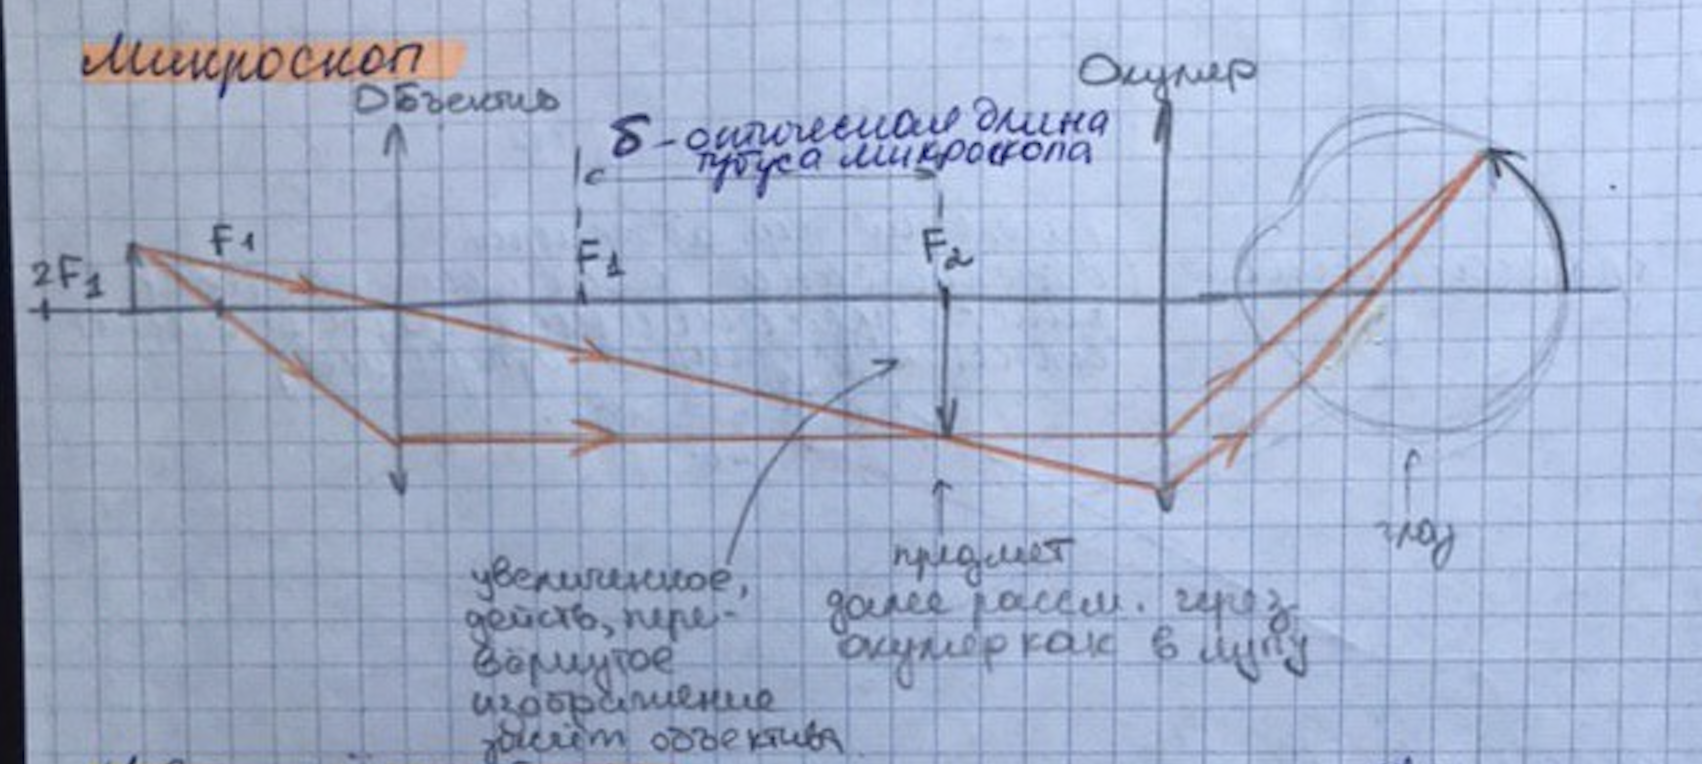
\includegraphics[width=\textwidth]{6_3}
	\caption{Микроскоп. Извините, я усталь.}
\end{figure}

\subsection{Труба Кеплера}

\begin{figure}[H]
	\centering
	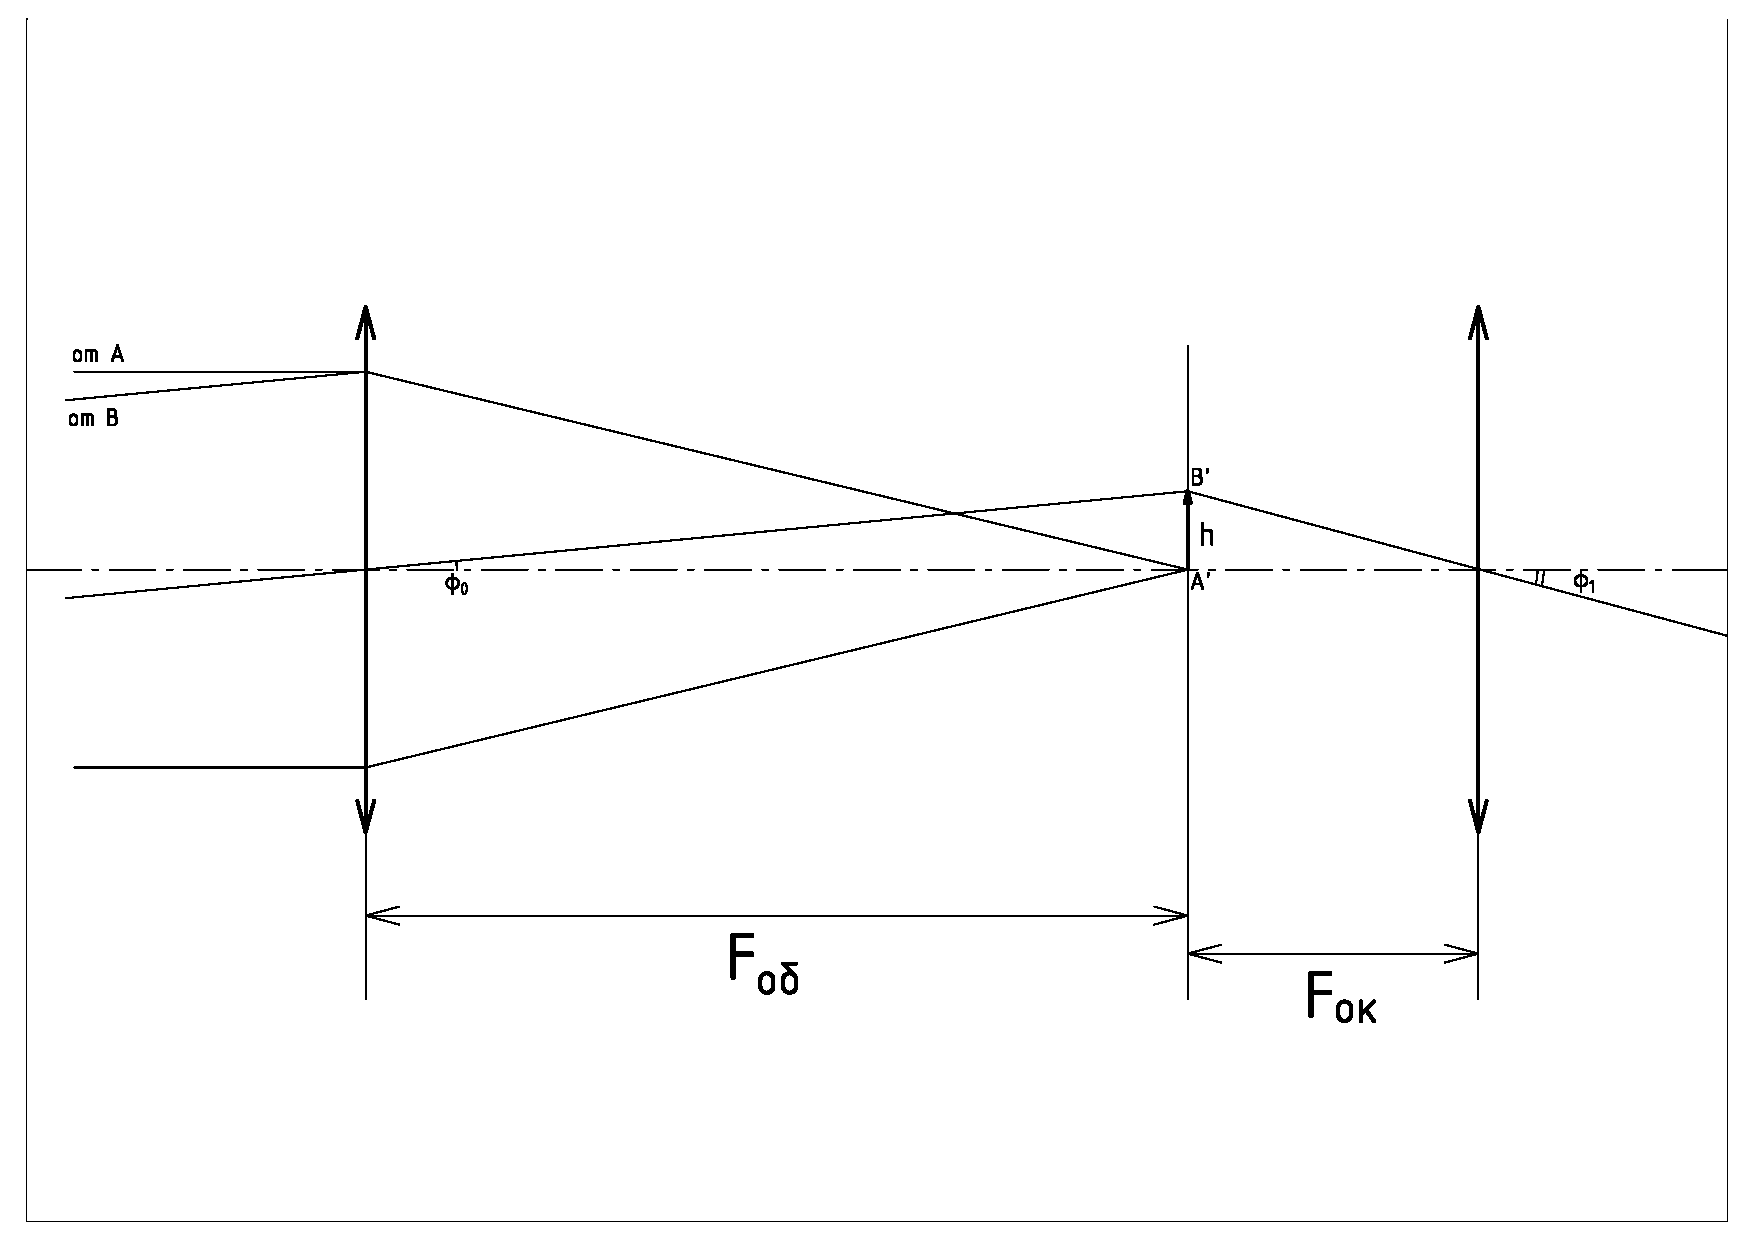
\includegraphics[width=\textwidth]{6_1}
	\caption{Труба Кеплера}
\end{figure}

Из подобия мы сразу можем заявить:

\begin{equation*}
	\frac{D_{\text{об}}}{F_{\text{об}}} = \frac{D_{\text{ок}}}{F_{\text{ок}}}
\end{equation*}

Где $D$ --- диаметр.

Пусть мы наводимся на далекий объект (луну, например). Рассмотрим два пучка от точки $A$ и $B$ соответственно. При прохождении через первую линзу они дадут изображение $A'B'$ в фокальной плоскости, пусть его высота $h$. Затем луч от точки $B$ выйдет из второй линзы (окуляра) под углом $\phi_1$. Введем \textbf{угловое увеличение телескопа} $\gamma$:

\begin{equation*}
	\gamma = \frac{\tg \phi_1}{\tg\phi_0} = \frac{h / F_{\text{ок}}}{ h / F_{\text{об}}} = \frac{F_{\text{об}}}{F_{\text{ок}}} = \frac{D_{\text{об}}}{D_{\text{ок}}}
\end{equation*}

\subsection{Труба Галилея}

В случае трубы Галилея ситуация ровно такая же, как в случае трубы Кеплера, однако линза окуляра рассеивающая, а не собирающая. Из-за этого фокус объектива должен совпасть с \textbf{задним} фокусом окуляра (см. рисунок). Больше от этого ничего не меняется.

\begin{figure}[H]
	\centering
	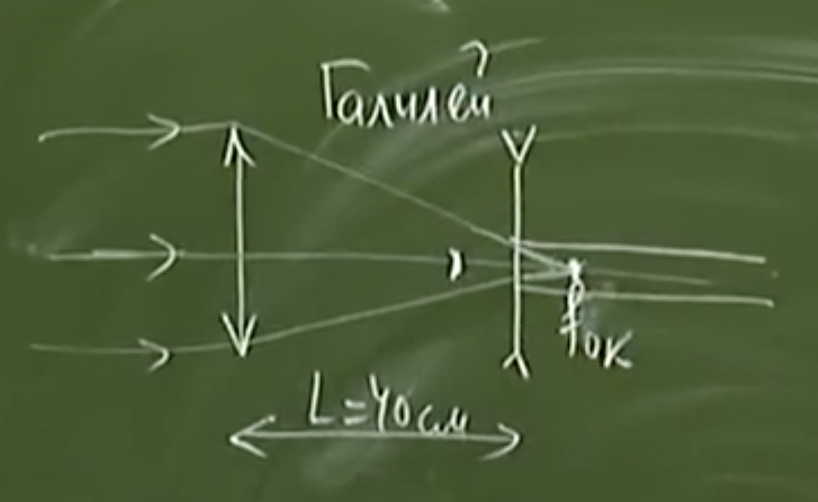
\includegraphics[width=\textwidth]{6_2}
	\caption{Труба Галилея}
\end{figure}

	
	\newpage
	
	
	\section{Плоская монохроматическая волна. Представление монохроматических волн в
		комплексном виде. Сферическая и цилиндрическая волны. Стоячие электромагнитные
		волны. Опыты Винера.}
	(ЛЛ2 \S 46 и дальше)\\
	\subsection*{Плоские волны}
	Стартуем с обычного волнового уравнения:
	\begin{align*}
	\Delta A - \dfrac{1}{c^2} \dfrac{\partial^2}{\partial t^2}A = 0
	\end{align*}
	Где A - это вектор потенциал, так же помним что такое уравнение было полученно при калибровке $\diver A = 0$. Понятно, что для напряженности электрического и магнитного поля верны такие же уравнения. Хотим изучать плоские волны, это значит, что вектор потенциал может зависить только от одной координаты. Для определенности это x. Тогда уравнение выглядит так:
	\begin{align}
	\dfrac{\partial^2}{\partial x^2}\vec{A} - \dfrac{1}{c^2} \dfrac{\partial^2}{\partial t^2}\vec{A} = 0
	\label{7_1eq}
	\end{align}
	Калибровочное условие превращается в $ \dfrac{\partial}{\partial x}A_x = 0$, значит $\dfrac{\partial^2}{\partial t^2}A_x  = 0$. Отсюда логично заключить, что x компонента потенциала либо линейна по времени, либо ее нет. Первое означало бы наличие постоянного электрического поля, что никакого отношения к волнам не имеет. Значит $A_x = 0$. То есть вектор потенциал всегда лежит в плоскости перпендикулярной направлению движения. Для любого, кто читал конспект по матфизу очевидно, что решением уравнения (\ref{7_1eq}) будет любая функция $\vec{A}(t - \dfrac{x}{c})$ понятно что волна еще может лететь влево, но опустим это, там все то же самое. Из этого решения следует, что 
	\begin{align}
	\dfrac{\partial A}{\partial t} = -\dfrac{1}{c} \dfrac{\partial A}{\partial x}
	\label{7_2eq}
	\end{align}
	Пока запомним это. Теперь вычислим E и H, помня, что вектор потенциал зависит только от x
	\begin{align*}
	\vec{H} = - \vec{e}_y \partial_x A_z + \vec{e}_z \partial_x A_y\\
	\vec{E} = -\dfrac{1}{c} \vec{e}_y\dfrac{\partial A_y}{\partial x} -\dfrac{1}{c} \vec{e}_z \dfrac{\partial A_z}{\partial x}\\
	\vec{E}\vec{H} = -\dfrac{1}{c^2} \partial_x A_y \partial_x A_z +\dfrac{1}{c^2} \partial_x A_y \partial_x A_z = 0
	\end{align*}
	Здесь мы воспользовались формулой (\ref{7_2eq}). Теперь мы знаем, что в любой плоской волне электрическое поле перпендикулярно электрическому. И лежат они в одной плоскости, перпендикулярной направлению распространения волны. Кстати, по модулю они равны, что видно из уравнений выше. Так что можно смело написать:
	\begin{align*}
	S = \dfrac{c}{4\pi} [\vec{E} \vec{H}] = \dfrac{c E^2}{4\pi}\vec{n} = \dfrac{cH^2}{4\pi}\vec{n}
	\end{align*}
	Где вектор n единичный в направлении распространения. \\
	Что такое монохроматическая волна? Это когда $\dfrac{1}{c^2} \dfrac{\partial^2}{\partial t^2}\vec{A} =- \dfrac{\omega^2}{c^2} \vec{A}$, фактически фурье компонента. Если подставить это в уравнение (\ref{7_1eq}), то получим обычное уравнение на гармонический осциллятор для координаты. Значит итоговое решение будет:
	\begin{align*}
	\vec{A} = 	Re\{ \vec{A}_0 e^{-i \omega (t - x/c)}\}
	\end{align*}
	Действительную часть мы взяли потому, что поля не бывают комплексными. А вот $A_0$ бывает. Поэтому правильным выбором $A_0$ волну можно сделать любой комбинацией синусов и косинусов которая нужна. Если взять от этой штуки частную производную по времени, что получить поле не сложно:
	\begin{align*}
	\vec{E} = 	Re\{ \vec{E}_0 e^{-i \omega (t - x/c)}\}
	\end{align*}
	Введя вектор $\vec{k} = \dfrac{\omega}{c} \vec{n}$ можно отвязаться от координат и просто написать
	\begin{align*}
	\vec{E} = 	Re\{ \vec{E}_0 e^{i (kr - \omega t)}\}
	\end{align*}
	Обычно взятие действительной части опускают. Так пока мы совершаем линейные операции с полями нам это не важною.  \\
	\subsection*{Сферические и цилиндрические волны}
	Для простоты рассмотрим только монохроматические. Сферические волны это когда зависимость есть только от расстояния до начала координат. Вспоминая как вылгядит оператор лапласа в сферике (например в вики) и быстро решая уравнение получаем (Re опустил):
	\begin{align*}
	A = A_0 \dfrac{e^{i (kr - \omega t)}}{r}
	\end{align*}
	Теперь пишем дифур на цилиндрические волны. \textbf{Здесь r - расстояние до оси}
	\begin{align*}
	&\dfrac{1}{r} \partial_r (r \partial_r f) + k^2 f = 0\\
	& x = r k\\
	&f'' + \dfrac{1}{x} f' + f = 0
	\end{align*} 
	А это уравнение на функцию Бесселя. Конечно есть еще функция Неймана, но нам надо чтобы в нуле значение было конечным, а функция Неймана этого не дает. Итого решениe пропорцианально такой штуке: $J_0(k r) e^{-i\omega t}$ на больших временах можно написать асиптотику: 
	\begin{align*}
	A_0 \dfrac{e^{i (kr - \omega t - \pi/4)}}{\sqrt{r}}
	\end{align*}
	\subsection*{Стоячие волны и опыт Винера}
	Если есть две одинаковые волны $e^{i (kr - \omega t)} \quad e^{i (-kr - \omega t)}$, идущие в разных направлениях (например после отражения), то их можно сложить и получить $2\cos \omega t \cos k r$\\
	Но физически мы можем заметить только квадрат амплитуды. Ну тут видно, что после усреднения по времени мы будем наблюдать серию кучностей на расстоянии по $\lambda/2$ друг от друга. Проблема в их наблюдении это малая длина волны. Вот что придумал Винер.\\
	Берем фоточувствительную пластинку и ставим ее под малым углом к зеркалу. Освещаем зеркало монохроматическим светом на наблюдаем тучности непосредственно
	\begin{figure}[H]
		\centering
		\includegraphics[scale = 0.3]{7_1}
	\end{figure}
	Расстояние между ними по прямой будет $\dfrac{\lambda}{2 \sin \alpha}$, то есть зная синус наклона можно узнать и длину волны.  
	
	\newpage
	
	\section{Электромагнитные волны в однородных, изотропных диэлектрических средах. Уравнения Максвелла. Поперечность электромагнитной волны. Взаимная
ориентация волнового вектора, векторов электрического и магнитного полей в
плоской волне. Стоячие электромагнитные волны. Опыты Винера.}
\noindent\rule{\textwidth}{0.5pt}

\subsection{Ликбез}

\textbf{Изотропной} среда называется если её физические свойства ($\epsilon$, $\mu$, $\sigma$ и другие) не зависят от направления\\ \\
\textbf{Электромагнитной} волна называется потому что характеризуется двумя взаимно ортогональными векторами: \textbf{E} и \textbf{H} - векторами напряженности электрического и магнитного полей, в процессе колебаний электрическое поле постепенно переходит в магнитное, магнитное — в электрическое.\\ \\
\textbf{Фронтом} волны называют поверхность, до которой дошёл волновой процесс к данному моменту времени. По форме волнового фронта выделяют простейшие волны: сферическую, плоскую, цилиндрическую. Нормаль к волновому фронту совпадает с направлением распространения волны в данной точке.\\ \\
\textbf{Плоская волна} - волна, фронт у которой плоский (движущиеся в пространстве параллельные плоскости).\\ \\
\textbf{Волновой вектор} - вектор, направление которого перпендикулярно фазовому фронту бегущей волны, а абсолютное значение равно волновому числу.\\ \\
\textbf{Волновое число} - отношение $2 \pi$ радиан к длине волны\\ \\
Исходной системой для определения электромагнитного поля в среде является система \textbf{уравнений Максвелла}:
\\
\begin{spacing}{0.7}
$$ rot  \textbf{H} = \frac{1}{c} \frac{\partial \textbf{D}}{\partial t} + 
\frac{4\pi}{c} \textbf{j}, \eqno{(1)}$$
\\
$$ rot \textbf{E} = -\frac{1}{c} \frac{\partial \textbf{B}}{\partial t},\eqno{(2)} $$
\\
$$ div \textbf{D} = 4 \pi \rho, \eqno{(3)} $$
\\
$$ div \textbf{B} = 0. \eqno{(4)}  $$\\

\end{spacing}

Здесь \textbf{E} и \textbf{H} - напряженности электрического и магнитного полей, \textbf{B} и \textbf{D} - векторы электрической и магнитной индукции, $\textbf{j}$ и $\rho$ - плотности токов и электрических зарядов в среде, их появление связано с действием электромагнитного поля, между собой они связаны уравнением непрерывности:

$$ div \textbf{j} + \frac{\partial \rho}{\partial t} = 0, \eqno{(5)}$$ 

Оно отражает закон сохранения полного электрического заряда внутри объема среды.\\ 
Уравнение (3) является следствием уравнений (1) и (5) (дивергенция от обоих частей (1), использование (5)), а (4) может быть получено из (2) (дивергенция от обоих частей (2), $div \ rot E = 0$), поэтому 
система уравнений (1) - (5) не является полной и для её решения относительно \textbf{E}, \textbf{H}, \textbf{B}, \textbf{D} и \textbf{j} надо дополнить систему тремя материальными уравнениями:

$$  \textbf{D} = \textbf{D}(\textbf{E}), \ \textbf{B}=\textbf{B}(\textbf{H}), \  \textbf{j = \textbf{j}}(\textbf{E})$$

Для однородной изотропной среды с диэлектрической проницаемостью $\epsilon$, магнитной проницаемостью $\mu$ и удельной проводимостью $\sigma$ эти уравнения принимают вид:

$$  \textbf{D} = \epsilon (\textbf{E}),  \textbf{B} = \mu (\textbf{H}), \textbf{j} = \sigma (\textbf{E})$$

\subsection{Уравнения Максвелла}

Для диэлектрической среды $\sigma = 0$ уравнения Максвелла перепишутся в виде:

\begin{spacing}{0.7}
$$ rot  \textbf{H} = \frac{\epsilon}{c} \frac{\partial \textbf{E}}{\partial t}, $$
\\
$$ rot \textbf{E} = -\frac{\mu}{c} \frac{\partial \textbf{H}}{\partial t}, $$
\\
$$ div \textbf{E} = 0,  $$
\\
$$ div \textbf{H} = 0. $$
\end{spacing}

\subsection{Электромагнитные волны в однородных, изотропных диэлектрических средах}

Исключая из системы \textbf{H} ($rot \ rot \textbf{E}  = grad \ div \textbf{E} - \nabla^2 \textbf{E}  = - \nabla^2 \textbf{E},$ получим уравнение на вектор \textbf{E}: 

$$ {\nabla}^2\textbf{E} - \frac{\epsilon \mu}{c^2} \frac{{\partial}^2 \textbf{E}}{\partial t^2} = 0$$

И такое же на \textbf{H}:

$$ \ {\nabla}^2\textbf{H} - \frac{\epsilon \mu}{c^2} \frac{{\partial}^2 \textbf{H}}{\partial t^2} = 0$$

Если искать решения данных уравнений в виде монохроматических (строго гармонических волн с постоянной во времени частотой, амплитудой и начальной фазой) волн, то получаем:

$$ {\nabla}^2\textbf{E} + k^2 \textbf{E} = 0, \ \ \ {\nabla}^2\textbf{H} + k^2 \textbf{H} = 0, \ \ \ k = \frac{\omega}{c}\sqrt{ \epsilon \mu}$$

Здесь $k$ - величина комплексного \textbf {волнового вектора} $\textbf{k} = k \textbf{s},$ где \textbf{s} - единичный вектор в направлении распространения волны. Его удобно представлять в виде $k = k_0(n -ik),$ где $k_0 = \frac{\omega}{c}$, а $n$ и $k$ называются коэффициентами преломления и поглощения соответственно.\\ \\

\subsection{Взаимная ориентация волнового вектора, векторов электрического и магнитного полей в плоской волне}


Эти три вектора образуют правую тройку векторов.

Векторы \textbf{E} и \textbf{H} могут быть представлены в виде:
$$ \textbf{E} = A_1 \exp{(i(\omega t - \textbf{k}\textbf{r}))}, \ \textbf{H} = A_2 \exp{(i(\omega t - \textbf{k}\textbf{r}))}$$
Связь между ними следует из закона электромагнитной индукции Фарадея:
$$ rot \textbf{E} = - i [\textbf{k}, \textbf{E}] = -i\frac{\omega}{c} \sqrt{n^2 + k^2} [\textbf{s}, \textbf{E}] \exp{(-i \arctg{(\frac{k}{n})})}$$
Отсюда:
$$ \textbf{B} = \sqrt{n^2 + k^2}[\textbf{s}, \textbf{E}] \exp{(-i \arctg{(\frac{k}{n})})}$$


\subsection{Поперечность электромагнитной волны}

Чтобы определить структуру волн, а именно доказать их \textbf{поперечность} перейдём к рассмотрению поля в котором векторы \textbf{E} и \textbf{H} зависят от одной пространственной координаты $\xi = (\textbf{m}\textbf{r})$ ($+m$ - направление распространения волны) и времени $t$, тогда:

$$ div \textbf{E} = \frac{\partial}{\partial \xi} (\textbf{m}\textbf{E}),
\ \ \ rot \textbf{E} = \frac{\partial}{\partial \xi}[\textbf{m}\textbf{E}],$$
Уравнения Максвелла для такой системы:

$$\frac{\partial}{\partial \xi}[\textbf{m}\textbf{H}] = \frac{\epsilon}{c} \frac{\partial \textbf{E}}{\partial t},$$

$$\frac{\partial}{\partial \xi}[\textbf{m}\textbf{E}] = -\frac{\mu}{c} \frac{\partial \textbf{H}}{\partial t},$$ 

$$\frac{\partial}{\partial \xi} (\textbf{m}\textbf{E}) = \frac{\partial \textbf{E}_\xi}{\partial \xi} = 0$$

$$\frac{\partial}{\partial \xi} (\textbf{m}\textbf{H}) = \frac{\partial \textbf{H}_\xi}{\partial \xi}  = 0$$
\\ \\
Значит, проекции векторов  \textbf{E} $\textbf{E}_\xi $ и \textbf{H} $\textbf{H}_\xi $ на направление распространения волны могут зависить только от времени. Умножая первые два уравнения скалярно на \textbf{m}, получаем:
$$ \frac{\partial \textbf{E}_\xi}{\partial t} = \frac{\partial \textbf{H}_\xi}{\partial t} = 0$$
Т.е. проекции не зависят так же и от времени, что означает что электромагнитные волны в диэлектрической среде являются поперечными волнами, векторы \textbf{E} и \textbf{H} лежат в плоскости фронта волны.\\ \\

\subsection{Стоячая волна}

\textbf{Стоячая волна} есть результат суперпозиции двух электромагнитных волн бегущих навстречу друг другу:

Если первая волна распространяется в положительном направлении оси x и задается: $$E_y = E_m \cos{(\omega t - kx)},\ \ H_z = H_m \cos{(\omega t - kx)},$$ то уравнение волны бегущей в обратном направлении получается если заменить в скобках минусы на плюсы, учитывая что векторы \textbf{E}, \textbf{H}, \textbf{k} должны составлять правую тройку. Уравнение встречной:
$$E_y = E_m \cos{(\omega t + kx)}, \ \ H_z = -H_m \cos{(\omega t + kx)}$$

Результирующая:
$$E_y = 2E_m \cos{(kx)}\cos{(\omega t)}, \ \ H_z = 2H_m \sin{(kx)}\sin{\omega t)}$$

Колебания векторов \textbf{E}, \textbf{H} сдвинуты по фазе на $\pi/2$, для амплитудных значений $E_m$ и $H_m$ выполняется соотношение:

$$E_m \sqrt{\epsilon \epsilon_0} = H_m \sqrt{\mu \mu_0}$$

Если в некоторый момент $ E_y$ во всех точках имело максимальное значение и при этом $ H_z =0$, то через четверть периода картина будет обратной: $ H_z$ достигнет всюду максимальных значений со сдвигом в пространстве на $ \lambda/4$, а $ E_y$ обратится в нуль. 
\\ 

\subsection{Опыт Винера}


\begin{figure}[H]
	\centering
	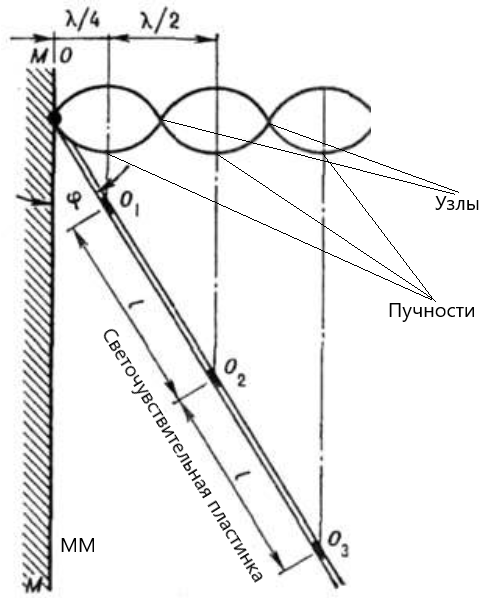
\includegraphics[scale = 0.5]{Viner}
\end{figure}

На плоское металл.зеркало (ММ)  направляется по нормали монохроматич. свет длиной волны  $\lambda$ . При отражении световых волн от этой поверхности образуются стоячие волны, узловые плоскости к-рых параллельны MМ и отстоят друг от друга на расстоянии $\frac{\lambda}{2}$ ; при этом на поверхности находятся узел электрич. вектора (E=0) и пучность магн. вектора. Под малым углом к поверхности зеркала располагается стеклянная пластинка с тонким $\frac{\lambda}{20}$  светочувствит. слоем эмульсии. Светочувствит. слой пересекался с пучностями векторов стоячей волны по прямым, параллельным поверхности зеркала. После  проявления на пластинке возникает система параллельных тёмных полос (O1, O2, O3), соответствующих местам макс. выделения серебра. Винер установил, что первая тёмная полоса располагается не на краю светочувствит. слоя, граничащего с металлич. зеркалом, а отстаёт от него на $\frac{\lambda}{4}$. Именно на этом расстоянии располагается первая пучность (пучность — точка или область в пространстве, в которой амплитуда максимальна и равна сумме амплитуд интерферирующих волн (амплитуда стоячей волны в пучностях вдвое больше амплитуды каждой из интерферирующих волн) электрической световой волны, т. е. фотографическое действие световой волны связано с её электрич. вектором.
	
	\newpage
	
	


\section{Линейно, циркулярно и эллиптически поляризованный свет. Поляризация естественного света. Степень поляризации. Поляризаторы. Закон Малюса}

\textit{Поляризацией} называется характеристика векторных волновых полей, описывающая поведение вектора колеблющейся величины в плоскости, перпендикулярной направлению распространения волны.

\textit{Плоскостью поляризации} называется плоскость, построенная на векторах $(E,k)$.
\subsection{Типы поляризации}
Плоская волна называется \textit{линейно поляризованной}, если ориентация плоскости поляризации не меняется во времени, то есть вектор напряженности электрического поля $E$ всегда лежит в одной и той же плоскости, содержащей вектор $k$.

В естественном (неполяризованном) свете плоскость поляризации меняется случайным образом (при этом вектор $E$ остается перпендикулярным волновому вектору $k$).

Выберем систему координат таким образом, что вектор $k$ направлен вдоль оси $z$, а вектор $E$ лежит в плоскости $(x, y)$.Пусть частота колебаний поля равна $\omega$. Тогда для компонент поля можно записать выражения

\begin{equation*}
    E_x = E_{x0}\cos(\omega t +\phi_x)
\end{equation*}


\begin{equation*}
    E_y = E_{y0}\cos(\omega t +\phi_y)
\end{equation*}

Если разность фаз этих величин равна 

\begin{equation*}
    \delta = \phi_x - \phi_y = 0, \pm\pi,
\end{equation*}


то вектор $E$ совершаеет колебания вдоль фиксированной прямой. Этот случай отвечает линейно поляризованной волне.

Если сдвиг фаз колебаний проекций отличается, то вектор $E$ совершаем вращение. В этом случае говорят, что свет имеет \textit{эллиптическую поляризацию}. Получим уравнение кривой, описываемой концом вектора $E$:

\begin{equation*}
    \left(\frac{E_x}{E_{x0}}\right)^2+\left(\frac{E_y}{E_{y0}}\right)^2 - 2\frac{E_x}{E_{x0}}\frac{E_y}{E_{y0}}\cos\delta = \sin^2\delta.
\end{equation*}

Здесь $\delta = \phi_x -\phi_y$ для сдвига фаз колебаний проекций $E_x$ и $E_y$.

Если окажется
\begin{equation*}
    \delta = \phi_x - \phi_y = \pm \frac{\pi}{2}, E_{x0} = E_{y0},
\end{equation*}

то описываемая вектором $E$ кривая есть окружность. В этом случае говорят о \textit{круговой поляризации}.

Круговая поляризация бывает двух типов - \textit{левая} и \textit{правая}. Если смотреть навстречу волновому вектору, то левой поляризации отвечает вращение вектора $E$ \textit{против часовой стрелки}. В случае правой поляризации вектор $E$ вращается \textit{по часовой стрелке}.
\subsection{Степень поляризации}

Говорят, что свет \textit{частично поляризован}, если он представляет собой смесь полностью поляризованного и естественного (неполяризованного) излучения. Пусть интенсивности этих компонент равны соответственно $I_{\text{пол}}$ и   $I_{\text{ест}}$. Тогда суммарная интенсивность составляет 
\begin{equation*}
    I_0 = I_{\text{пол}}+I_{\text{ест}}.
\end{equation*}

\textit{Степенью поляризации излучения называется отношение}


\begin{equation*}
    P = \frac{I_{\text{пол}}}{I_0} = \frac{I_{\text{пол}}}{I_{\text{пол}}+I_{\text{ест}}}.
\end{equation*}
\subsection{Поляризаторы}

\textit{Поляризатором} называют прибор, предназначенный для получения полностью или частично поляризованного оптического излучения.

Действие поляризаторов, создающих линецно поляризованный свет, основано, в частности, на следующий явлениях:

\begin{enumerate}
    \item линейный дихроизм,
    \item поляризация при отражении,
    \item поляризация при рассеянии,
    \item двойное лучепреломление.
\end{enumerate}

\subsection{Закон Малюса}

Найдем интенсивность волны, прошедшей через поляроид. Для этого разложим вектор $\textbf{E}$ на две компоненты - вдоль и поперек оси поляроида.

\begin{equation*}
    E_z = E\cos \phi, E_x = E\sin \phi
\end{equation*}

Через поляроид пройдет волна с поляризацией $E_z$. Другая же волна (с поляризацией $E_x$) полностью поглощается веществом. В итоге через поляроид проходит свет, поляризованный вдоль оси поляроида, причем его интенсивность ($I_{\text{прош}} \sim E_z^2$) равна

\begin{equation*}
    I_{\text{прош}} = I_0 \cos^2 \phi,
\end{equation*}

$I_0 \sim E^2 = E_x^2 + E_z^2$ - интенсивность волны, падающей на поляроид. Это соотношение называется законом Малюса.




	
	\newpage
	
	\section{Аберрации оптических систем. Аберрации, обусловленные зависимостью показателя преломления от длины волны (хроматические аберрации).}
\subsection{Аберрации оптических систем.}
\begin{definition}
	\textbf{Аберрации оптических систем} (лат. aberratio - уклонение),
	погрешности изображений, даваемых оптическими системами.
	Проявляются в том, что оптические изображения в ряде случаев не
	вполне отчётливы, не точно соответствуют объекту или оказываются
	окрашенными.
\end{definition}
Аберации делят на \textbf{\textit{монохроматические (геометрические)}} и \textbf{\textit{хроматические}}, среди геометрических ывделяют
\begin{itemize}
	\item Сферическая аберрация
	\item Кома
	\item Астигматизм
	\item Дисторсия 
	\item Кривизна поля (поверхности) изображения
\end{itemize}
\subsubsection{Классификация геометрических аберраций}
Геометрические аберрации практичеки всегда являются учётом непараксиальности в ходе лучей. Произвольный луч в пространстве можно задать, указав прямоугольные координаты $y$, $z$, $\eta$ и $\zeta$ точек его пересечения с  предметной плоскостью (т.е. плоскостью, проходящей через изображаемую точку $P$ перпендикулярно к главной оптической оси) и плоскостью входного зрачка. После прохождения через оптическую систему луч пересечёт плоскость параксиального изображения в точке с координатами $y'$ и $z'$. Координаты самого параксиального изображения (\textit{параксиального фокуса}) -- $y_{0}'$, $z'_{0}$. Разности
\begin{align*}
\Delta y' &= y' - y'_{0} & \Delta z' &= z'- z'_{0}
\end{align*} 
примем за меру отступления от предельного случая параксиальной оптики.
Координаты $y'$  и  $z'$ будут функциями $y$, $z$, $\eta$ и $\zeta$:
\begin{align*}
y' &= f_{y}(y,z,\eta,\zeta) & z' &= f_{z}(y,z,\eta,\zeta)
\end{align*}
Линейные члены разложений $f_{y}$ и $f_{z}$ не зависят от $\eta$ и $\zeta$ и соответствуют параксиальной оптике, члены чётных степеней не войдут в эти разложения в силу осевой симметрии оптической задачи. Поэтому $\Delta y'$ и $\Delta z'$ будут определятся третьими членами разложения $f_{y}$ и $f_{z}$ (пожтому часто рассматриваемые дальше аберрации называются аберрациями третьего порядка).

Введём три вектора, перпендикулярных главной оптической оси системы:
\begin{align*}
\mathbf{r} &= y\mathbf{j} + z\mathbf{k} & \mathbf{r}' &= y'\mathbf{j} + z'\mathbf{k} & \bm{\sigma} &= \eta\mathbf{j} + \zeta\mathbf{k}
\end{align*}
Тогда вектор 
\begin{equation*}
\Delta \mathbf{r}' = \Delta y'\mathbf{j} + \Delta z'\mathbf{k}
\end{equation*}
может быть разложен по векторам $\mathbf{r}$ и $\bm{\sigma}$.
Причём в виду симметрии коэффициенты этих разложения могут зависеть только от <<инвариантов вращения>> $\bm{\sigma}^{2}$, $(\bm{\sigma}\mathbf{r})$ и $r^{2}$:
\begin{equation}
\label{series3}
\Delta \mathbf{r}' \approx \Big(A\bm{\sigma}^{2} + B(\bm{\sigma}\mathbf{r}) + C\mathbf{r}^{2}\Big)\bm{\sigma} + \Big(D\bm{\sigma}^{2} + E(\bm{\sigma}\mathbf{r}) + F\mathbf{r}^{2}\Big)\mathbf{r}
\end{equation}
В дальнейшем под $|\bm{\sigma}|$ понимается радиус входного зрачка. \textit{Аберрационной} кривой называют кривую, по которой плоскость параксиального изображения пересекает пучок лучей, проведённых из точки-объекта $P$ через окружность входного зрачка. Изображением вместо точки теперь окажется область, ограниченная аберрационной кривой.

Каждый из постоянных коэффициентов $A$, $B$, $C$, $D$, $E$ и $F$ в уравнении (\ref{series3}) определяется конфигурацией оптической системы и отвечает за конкретный тип аберрации. Аберрация определяемая членом $A\bm{\sigma}^{2}\bm{\sigma}$ называется \color{blue}{сферической}\normalcolor. Членам $B(\bm{\sigma}\mathbf{r})\bm{\sigma} + D\bm{\sigma}^{2}\mathbf{r}$ соответствует \color{blue}{кома}\normalcolor. Членам $C\mathbf{r}^{2}\bm{\sigma} + E(\bm{\sigma} r)\mathbf{r}$ -- \color{blue}{астигматизм косых лучей} \normalcolor и \color{blue}{искривление плоскости изображения}\normalcolor. Члену $F\mathbf{r}^{2}\mathbf{r}$  соответствует \color{blue}{дисторсия}\normalcolor.
\subsection{Хроматическая аберрация}
\begin{wrapfigure}{r}{0.55\textwidth}
	\begin{tikzpicture}[>=latex']
	\draw[black] (-2.598,-1.5) arc (210:150:3);
	\draw[black] (-2.4,-1.5) arc (-30:30:3);
	\draw[black] (-2.4,-1.5) -- (-2.598,-1.5); 
	\draw[black] (-2.4,1.5) -- (-2.598,1.5);
	\draw[black,->] (-4,-1.2) -- (-3,-1.2);
	\draw[black] (-4,-1.2) -- (-2.75,-1.2);
	\draw[black,->] (-4,1.2) -- (-3,1.2);
	\draw[black] (-4,1.2) -- (-2.75,1.2);
	\draw[red,->] (-2.75,1.2) -- (-2.22,1.15);
	\draw[green,->] (-2.75,1.2) -- (-2.2,1.1);
	\draw[blue,->] (-2.75,1.2) -- (-2.18,1.05);
	\draw[red,->] (-2.75,-1.2) -- (-2.22,-1.15);
	\draw[green,->] (-2.75,-1.2) -- (-2.2,-1.1);
	\draw[blue,->] (-2.75,-1.2) -- (-2.18,-1.05);
	\draw[red] (-2.22,1.15) -- (2,0);
	\draw[green] (-2.2,1.1) -- (1.5,0);
	\draw[blue] (-2.18,1.05) -- (1,0);
	\draw[red] (-2.22,-1.15) -- (2,0);
	\draw[green] (-2.2,-1.1) -- (1.5,0);
	\draw[blue] (-2.18,-1.05) -- (1,0);
	\draw[red,->] (-2.22,1.15) -- (-0.11,0.575);
	\draw[green,->] (-2.2,1.1) -- (-0.35,0.55);
	\draw[blue,->] (-2.18,1.05) -- (-0.59,0.525);
	\draw[red,->] (-2.22,-1.15) -- (-0.11,-0.575);
	\draw[green,->] (-2.2,-1.1) -- (-0.35,-0.55);
	\draw[blue,->] (-2.18,-1.05) -- (-0.59,-0.525);
	\draw[gray,dashdotted] (-4,0)--(2.5,0);
	\end{tikzpicture}
	\caption{Пример хроматической аберрации.}
	\label{chrom1}
\end{wrapfigure} 
Если используется белый свет, то в изображении возникают дополнительные аберрации. Это связано с тем, что показатель прломления зависит от длины волны (дисперсия света). Поэтому оптическая сиситема даёт не одно, а множнство монохроматических изображений, отличающихся друг от друга по величине и положению. Результирующее же изображение, получающееся от нложения таких монохроматических изображений, оказывается нерезким и с окрашенными краями. Это явление и называется \textit{хроматической аберрацией} (например рис.~\ref{chrom1}).
\begin{figure}[H]
	\centering
		\begin{tikzpicture}[>=latex']
	\draw[black] (-2.598,-1.5) arc (210:150:3);
	\draw[black] (-2.4,-1.5) arc (-30:30:3);
	\draw[black] (-2.4,-1.5) -- (-2.598,-1.5); 
	\draw[black] (-2.4,1.5) -- (-2.598,1.5);
	\draw[black,->] (-4,-1.2) -- (-3,-1.2);
	\draw[black] (-4,-1.2) -- (-2.75,-1.2);
	\draw[black,->] (-4,1.2) -- (-3,1.2);
	\draw[black] (-4,1.2) -- (-2.75,1.2);
	\draw[red,->] (-2.75,1.2) -- (-2.22,1.15);
	\draw[green,->] (-2.75,1.2) -- (-2.2,1.1);
	\draw[blue,->] (-2.75,1.2) -- (-2.18,1.05);
	\draw[red,->] (-2.75,-1.2) -- (-2.22,-1.15);
	\draw[green,->] (-2.75,-1.2) -- (-2.2,-1.1);
	\draw[blue,->] (-2.75,-1.2) -- (-2.18,-1.05);
	\draw[red] (-2.22,1.15) -- (2,0);
	\draw[green] (-2.2,1.1) -- (1.5,0);
	\draw[blue] (-2.18,1.05) -- (1,0);
	\draw[red] (-2.22,-1.15) -- (2,0);
	\draw[green] (-2.2,-1.1) -- (1.5,0);
	\draw[blue] (-2.18,-1.05) -- (1,0);
	\draw[red,->] (-2.22,1.15) -- (-0.11,0.575);
	\draw[green,->] (-2.2,1.1) -- (-0.35,0.55);
	\draw[blue,->] (-2.18,1.05) -- (-0.59,0.525);
	\draw[red,->] (-2.22,-1.15) -- (-0.11,-0.575);
	\draw[green,->] (-2.2,-1.1) -- (-0.35,-0.55);
	\draw[blue,->] (-2.18,-1.05) -- (-0.59,-0.525);
	\draw[gray,dashdotted] (-4,0)--(2.5,0);
	\end{tikzpicture}
	{\begin{tikzpicture}[>=latex']
		\draw[black] (-2.598,-1.5) arc (210:150:3);
		\draw[black,thick] (-2.4,-1.5) arc (-30:30:3);
		\draw[black] (-2.4,-1.5) -- (-2.598,-1.5); 
		\draw[black] (-2.4,1.5) -- (-2.598,1.5);
		\draw[black,->] (-4,-1.2) -- (-3,-1.2);
		\draw[black] (-4,-1.2) -- (-2.75,-1.2);
		\draw[black,->] (-4,1.2) -- (-3,1.2);
		\draw[black] (-4,1.2) -- (-2.75,1.2);
		\draw[red,->] (-2.75,1.2) -- (-2.22,1.15);
		\draw[green,->] (-2.75,1.2) -- (-2.2,1.1);
		\draw[blue,->] (-2.75,1.2) -- (-2.18,1.05);
		\draw[red,->] (-2.75,-1.2) -- (-2.22,-1.15);
		\draw[green,->] (-2.75,-1.2) -- (-2.2,-1.1);
		\draw[blue,->] (-2.75,-1.2) -- (-2.18,-1.05);
		\draw[black] (-2.4,1.5) -- (-1.6,1.5) -- (-1.6,-1.5) -- (-2.4,-1.5);
		\draw[gray,dashdotted] (-4,0)--(2.5,0);
		%
		\draw[red,->] (-2.22,1.15) -- (-1.6,1.075);
		\draw[green,->] (-2.2,1.1) -- (-1.6,1.05);
		\draw[blue,->] (-2.18,1.05) -- (-1.6,1.03);
		\draw[red,->] (-2.22,-1.15) -- (-1.6,-1.075);
		\draw[green,->] (-2.2,-1.1) -- (-1.6,-1.05);
		\draw[blue,->] (-2.18,-1.05) -- (-1.6,-1.03);
		%
		\draw[red] (-1.6,1.075) -- (2.5,0);
		\draw[green] (-1.6,1.05) -- (2.3,0);
		\draw[blue] (-1.6,1.03) -- (2.1,0);
		\draw[red] (-1.6,-1.075) -- (2.5,0);
		\draw[green] (-1.6,-1.05) -- (2.3,0);
		\draw[blue] (-1.6,-1.03) -- (2.1,0);
		\draw[red,->] (-1.6,1.075) -- (0.45,0.5375);
		\draw[green,->] (-1.6,1.05) -- (0.35,0.525);
		\draw[blue,->] (-1.6,1.03) -- (0.25,0.515);
		\draw[red,->] (-1.6,-1.075) -- (0.45,-0.5375);
		\draw[green,->] (-1.6,-1.05) -- (0.35,-0.525);
		\draw[blue,->] (-1.6,-1.03) -- (0.25,-0.515);
		\end{tikzpicture}}
	\caption{Уменьшение хроматической аберрации при помощи рассеивающей линзы}
	\label{chrom_kor1}
\end{figure}
\begin{wrapfigure}{r}{0.55\textwidth}
	\centering
	\begin{tikzpicture}[>=latex']
	\draw[black] (-2.598,-1.5) arc (210:150:3);
	\draw[black] (-2.4,-1.5) arc (-30:30:3);
	\draw[black] (-2.4,-1.5) -- (-2.598,-1.5); 
	\draw[black] (-2.4,1.5) -- (-2.598,1.5);
	\draw[black,->] (-4,-1.2) -- (-3,-1.2);
	\draw[black] (-4,-1.2) -- (-2.75,-1.2);
	\draw[black,->] (-4,1.2) -- (-3,1.2);
	\draw[black] (-4,1.2) -- (-2.75,1.2);
	\draw[red,->] (-2.75,1.2) -- (-2.22,1.15);
	\draw[green,->] (-2.75,1.2) -- (-2.2,1.1);
	\draw[blue,->] (-2.75,1.2) -- (-2.18,1.05);
	\draw[red,->] (-2.75,-1.2) -- (-2.22,-1.15);
	\draw[green,->] (-2.75,-1.2) -- (-2.2,-1.1);
	\draw[blue,->] (-2.75,-1.2) -- (-2.18,-1.05);
	\draw[red] (-2.22,1.15) -- (2,0);
	\draw[green] (-2.2,1.1) -- (1.5,0);
	\draw[blue] (-2.18,1.05) -- (1,0);
	\draw[red] (-2.22,-1.15) -- (2,0);
	\draw[green] (-2.2,-1.1) -- (1.5,0);
	\draw[blue] (-2.18,-1.05) -- (1,0);
	\draw[red,->] (-2.22,1.15) -- (-0.11,0.575);
	\draw[green,->] (-2.2,1.1) -- (-0.35,0.55);
	\draw[blue,->] (-2.18,1.05) -- (-0.59,0.525);
	\draw[red,->] (-2.22,-1.15) -- (-0.11,-0.575);
	\draw[green,->] (-2.2,-1.1) -- (-0.35,-0.55);
	\draw[blue,->] (-2.18,-1.05) -- (-0.59,-0.525);
	\draw[gray,dashdotted] (-4,0)--(2.5,0);
	\end{tikzpicture}
	{\begin{tikzpicture}[>=latex']
		\draw[black] (-2.598,-1.5) arc (210:150:3);
		\draw[black,thick] (-2.4,-1.5) arc (-30:30:3);
		\draw[black] (-2.4,-1.5) -- (-2.598,-1.5); 
		\draw[black] (-2.4,1.5) -- (-2.598,1.5);
		\draw[black,->] (-4,-1.2) -- (-3,-1.2);
		\draw[black] (-4,-1.2) -- (-2.75,-1.2);
		\draw[black,->] (-4,1.2) -- (-3,1.2);
		\draw[black] (-4,1.2) -- (-2.75,1.2);
		\draw[red,->] (-2.75,1.2) -- (-2.22,1.15);
		\draw[green,->] (-2.75,1.2) -- (-2.2,1.1);
		\draw[blue,->] (-2.75,1.2) -- (-2.18,1.05);
		\draw[red,->] (-2.75,-1.2) -- (-2.22,-1.15);
		\draw[green,->] (-2.75,-1.2) -- (-2.2,-1.1);
		\draw[blue,->] (-2.75,-1.2) -- (-2.18,-1.05);
		\draw[black] (-2.4,1.5) -- (-1.6,1.5) -- (-1.6,-1.5) -- (-2.4,-1.5);
		\draw[gray,dashdotted] (-4,0)--(2.5,0);
		%
		\draw[red,->] (-2.22,1.15) -- (-1.6,1.075);
		\draw[green,->] (-2.2,1.1) -- (-1.6,1.05);
		\draw[blue,->] (-2.18,1.05) -- (-1.6,1.03);
		\draw[red,->] (-2.22,-1.15) -- (-1.6,-1.075);
		\draw[green,->] (-2.2,-1.1) -- (-1.6,-1.05);
		\draw[blue,->] (-2.18,-1.05) -- (-1.6,-1.03);
		%
		\draw[red] (-1.6,1.075) -- (2.5,0);
		\draw[green] (-1.6,1.05) -- (2.0,0);
		\draw[blue] (-1.6,1.03) -- (2.5,0);
		\draw[red] (-1.6,-1.075) -- (2.5,0);
		\draw[green] (-1.6,-1.05) -- (2.0,0);
		\draw[blue] (-1.6,-1.03) -- (2.5,0);
		\draw[red,->] (-1.6,1.075) -- (0.45,0.5375);
		\draw[green,->] (-1.6,1.05) -- (0.2,0.525);
		\draw[blue,->] (-1.6,1.03) -- (0.45,0.515);
		\draw[red,->] (-1.6,-1.075) -- (0.45,-0.5375);
		\draw[green,->] (-1.6,-1.05) -- (0.2,-0.525);
		\draw[blue,->] (-1.6,-1.03) -- (0.45,-0.515);
		\end{tikzpicture}}
	\caption{Уменьшение хроматической аберрации при помощи ахроматической линзы (красный и синий луч собираются в один фокус)}
	\label{chrom_kor2}
\end{wrapfigure}

Аберрации хроматического типа не устраняются полностью, однако их эффект снижается использованием линз изготовленных из стекла с различными оптическими свойствами или использованием линз различной формы, например рис.~\ref{chrom_kor1}. В примере приведённый на рисунке наблюдается так называемый хроматизм положения, величина аберрации в нём обычно определяется расстоянием между фокусом синих и красных лучей, при помощи дополнительной линзы это расстояние удаётся уменьшить, однако чаще исползуется ахроматическая линза, которая собирает в один фокус два пучка света с разной длинной волны (чаще вссего синий и красный). Система линз, выполняющих сближение фокусов фокусов трёх лучей называется апохроматической, четырёх а — суперахроматической. Оставшиеся после ахроматизации хроматические аберрации называются вторичными.
\subsection{Подробнее}
Подробнее смотреть в Сивухине \S 13-17.
	
	\newpage
	
	\section{Оптические явления на границе раздела изотропных диэлектриков. Соотношения амплитуд падающей, отраженной и преломленной волн (формулы Френеля). Изменение фазы волны при отражении. Энергетические коэффициенты отражения и пропускания света. Коэффициент отражения для естественного света.}

% Дописать про изменение фазы волны при отражении -- вроде бы было в Овчинкине (семинары)?

% Коэффициент отражения -- ?????

При падении плоской волны на границу раздела двух изотропных диэлектриков, появляется две волны: преломленная (которая проходит границу раздела сред) и отраженная (не проходит), которые создаются за счет колебаний в диэлектриках, возбуждаемых падающей волной. Сразу быстро получим законы отражения и преломления.

\subsection{Законы отражения и преломления}

Пусть падающая волна имеет следующий вид:

\begin{equation*}
\vec{E} = \vec{E}_0 \cdot e^{-i (\omega t - \vec{k} \cdot r)}
\end{equation*}

В таком случае, из-за того, что колебания являются вынужденными, мы можем сказать, что $\omega = \omega_r = \omega_t$.

Кроме того, как мы знаем из курса электричества, существует уравнение на граничное условие для вектора $E$, которое в нашем случае принимает вид (для тангенциальных компонент):

\begin{equation*}
E_\tau + E_{r\tau} = E_{t\tau}
\end{equation*}

Возьмем любую точку на линии границы сред. В таком случае:

\begin{equation*}
A_1 e^{i \vec{k} \vec{x}} + B_1 e^{i \vec{k}_r \vec{x}} = C_1 e^{i \vec{k}_t \vec{x}}
\end{equation*}

Это в свою очередь значит, что должны быть равны между собой величины, стоящие в показателе экспоненты. С учетом того, как мы ввели углы, получаем:

\begin{equation}
k\sin\phi = k_r \sin \phi_r = k_t \sin\phi_t
\label{eq:reflection_and_refraction}
\end{equation}

При этом, как мы знаем, $k$ зависит от свойств среды, поэтому для падающей волны и отраженной:

\begin{equation*}
k = k_r = \frac{w}{c} \sqrt{\mu \epsilon}
\end{equation*}

А для преломленной:

\begin{equation*}
k_t = \frac{w}{c} \sqrt{\mu'\epsilon'}
\end{equation*}

Тогда из уравнения \ref{eq:reflection_and_refraction} получаем:

\begin{align*}
&\phi = \phi_r\\
&\frac{\sin\phi_t}{\sin\phi} = \frac{k}{k_t} = \frac{\sqrt{\epsilon\mu}}{\sqrt{\epsilon'\mu'}} = \frac{n}{n'}
\end{align*}

\subsection{Коэффициенты Френеля}

Разложим падающую волну $\vec{E}$ по двум составляющим: в плоскости, параллельной плоскости рисунка, и в плоскости, перпендикулярной ($E_\parallel$ и $E_\perp$ соответственно). Мы имеем следующие граничные условия:

\begin{align*}
&E_\tau + E_{r\tau} = E_{t\tau}\\
&H_\tau + H_{r\tau} = H_{t\tau}
\end{align*}

Мы также знаем соотношение, связывающее между собой $H$ и $E$: $H = \sqrt{\epsilon}E$ (пренебрегаем магнитными свойствами сред и считаем $\mu = 1$, а также не забываем, что $\vec{H} \perp \vec{E}$). Также вспоминаем, что $n = \sqrt{\epsilon}$. Тогда граничные условия принимают вид (с учетом проекций, см. рисунок):

\begin{figure}[H]
	\centering
	\subfigure[]{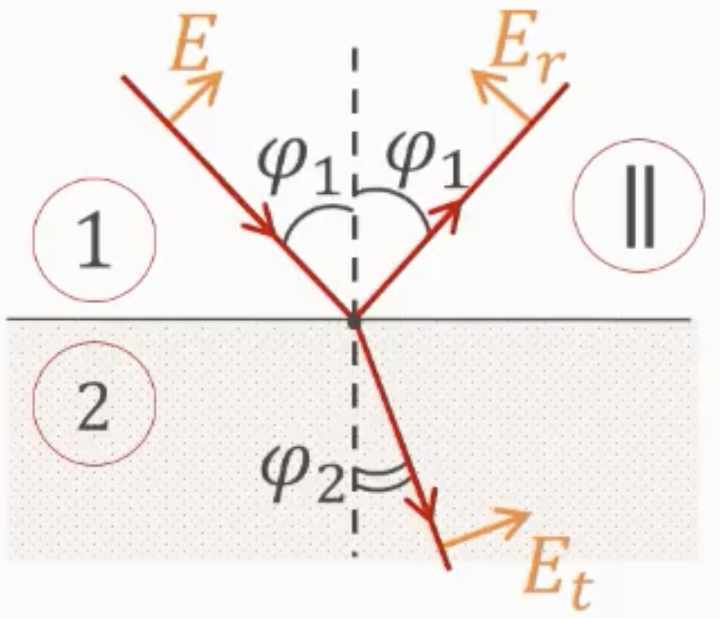
\includegraphics[width=0.48\linewidth]{11_1}
	}
	\subfigure[]{
	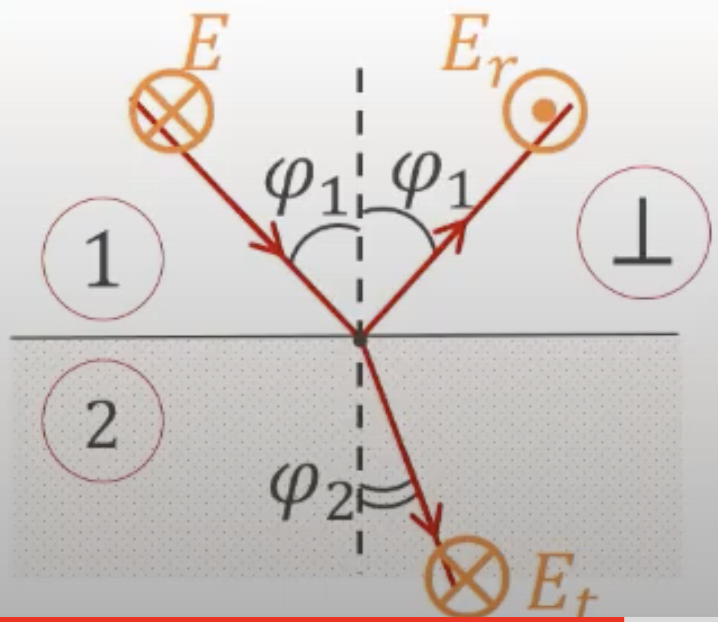
\includegraphics[width=0.48\linewidth]{11_2}
}
\end{figure}

\begin{align*}
&\begin{cases}
&E\cos\phi_1 - E_r\cos\phi_1 = E_t\cos\phi_2\\
&n_1 E + n_1 E_r = n_2 E_t\\
&\dfrac{\sin\phi_1}{\sin\phi_2} = \dfrac{n_2}{n_1}
\end{cases}
\quad &\text{--- для параллельной}\\
&\begin{cases}
&E - E_r = E_t\\
&n_1 E \cos\phi_1 + n_1 E_r \cos\phi_1 = n_2 E_t \cos\phi_2\\
&\dfrac{\sin\phi_1}{\sin\phi_2} = \dfrac{n_2}{n_1}
\end{cases}
\quad &\text{--- для перпендикулярной}\\
\end{align*}

Решив эту систему уравнений, мы получаем следующее:

\begin{align*}
&\begin{cases*}
E_r = \dfrac{\tg(\phi_1 - \phi_2)}{\tg(\phi_1 + \phi_2)}E\\
E_t = \dfrac{2\sin\phi_2\cos\phi_1}{\sin(\phi_1 + \phi_2) \cos(\phi_1 - \phi_2)}E
\end{cases*}
\quad &\text{--- для параллелльной}\\
&\begin{cases*}
E_r = \dfrac{\sin(\phi_2 - \phi_1)}{\sin(\phi_1 + \phi_2)}E\\
E_t = \dfrac{2\sin\phi_2\cos\phi_1}{\sin(\phi_1 + \phi_2)}E
\end{cases*}
\quad &\text{--- для перпендикулярной}
\end{align*}

Можно сразу же ввести энергетические коэффициенты отражения и пропускания света:

\begin{align*}
R_\parallel = \left(\frac{E_r}{E}\right)^2 = \frac{\tg^2\left(\phi_1 - \phi_2\right)}{\tg^2(\phi_1 + \phi_2)} \qquad T_\parallel = 1 - R_\parallel\\
R_\perp = \left(\frac{E_\perp}{E}\right)^2 = \frac{\sin^2(\phi_2 - \phi_1)}{\sin^2(\phi_2 + \phi_1)} \qquad T_\perp = 1 - R_\perp
\end{align*}
	
	\newpage
	
	\section{Поляризация отраженной и преломленной волн. Степень поляризации отраженного и преломленного света. Угол Брюстера. Физический смысл закона Брюстера.}

\textbf{Поляризация отражённой и преломлённой волн.}

	\begin{figure}[H]
	\centering
	\includegraphics*[width=\textwidth]{Otr}
    \end{figure}

$\phi$ --- угол падения, $\psi$ --- угол преломления;
$E_i$ --- амплитуда падающей волны, $E_r$ --- прошедшей.

Степень поляризации $$\boxed{\Delta = \frac{I_\perp - I_\parallel}{I_\perp + I_\parallel}}$$

Отношение отражённого потока к падающему:
$$r^2_\perp = [\frac{\sin{(\phi - \psi)}}{\sin{(\phi + \psi)}}]^2, \ r^2_\parallel = [\frac{\tan{(\phi - \psi)}}{\tan{(\phi + \psi)}}]^2$$

При $\phi \to \pi/2$ (скользящее падения): $r^2_\perp = r^2_\parallel = 1$ --- полное отражение.

При полном отражении фаза волны испытывает скачок $\delta_\perp$ и $\delta_\parallel$:
$$\tan{\frac{\delta_\perp}{2}} = \frac{\sqrt{\sin^2{\phi}-n^2}}{{\cos{\phi}}}, \ \tan{\frac{\delta_\parallel}{2}} = \frac{\sqrt{\sin^2{\phi}-n^2}}{{n^2\cos{\phi}}},$$
		
		Компоненты $E_r\perp$ и $E_r\parallel$ испытывают изменения фазы по отношению к $E_i\perp$ и $E_i\parallel$, причем $\delta_\perp$ отлично от $\delta_\parallel$. Для их разности справедливо $$\tan{\frac \delta 2 = \frac {\cos{\phi}\sqrt{sin^2{\phi} - n^2}}{\sin^2{\phi}}} \Rightarrow \tan{\frac \delta 2} > 0, \ 0< \delta< \pi.$$
		
		Если в падающей волне $E_i\perp$ и $E_i\parallel$ находятся в одной фазе, то в отраженном свете между $E_r\perp$ и $E_r\parallel$ появляется сдвиг фазы, зависящий от угла падения и показателя преломления. Таким образом, \textit{явление полного внутреннего отражения позволяет получить эллиптически-поляризованный свет.} Учитывая $0< \delta< \pi$, эллиптическая поляризация будет \textit{левой}.
		
		$\delta = 0$ при $\phi = \phi_{critical}$ и $\phi = \pi/2$ 
		Максимальный сдвиг $\delta_m$ при $\cos\phi = \sqrt \frac {(1 - n^2)}{(1+n^2)}$: $\tan \frac {\delta_m} 2 = \frac{1-n^2}{2n}$
		
		Для получения \textit{круговой поляризации} отражённого света, необходимо выполнение условий: $$E_r\parallel = \pm E_r\perp, \ \delta = \pi/2.$$
		Чтобы получить такой сдвиг при однократном отражении нужен $n = \sqrt2 - 1.$
		Для стекла можно подобрать такие значения угла падения, чтобы $\delta = \pi/4$, тогда при двукратном полном отражении в стекле происходило изменение фазы на $\pi/2$ (так действует пластинка в четверть волны).
		
	\begin{figure}[H]
	\centering
	\includegraphics*[width=0.4\textwidth]{ParFar}
    \end{figure}
Если $E_i\parallel = E_i\perp$ (плоскоть поляризаии составляет угол 45 градусов), то при полном внутреннем отражении $|E_r\parallel| = |E_r\perp|$ и при $\delta = \pi/2$ свет получится поляризованным по кругу.

\textbf{Явление Брюстера.}

Согласно \textit{формулам Френеля} коэффициент отражения параллельно поляризованной волны обращается в ноль при таком угле $\theta_B$, что $\tan{\theta_B = \frac{n_2}{n_1}}$, где $n_1$ --- показатель преломления среды, из которой падает луч, $n_2$ --- показатель преломления, в которую падает луч. Угол $\theta_B$ называется \textbf{углом Брюстера}.

	При падении под таким углом отражённая волна оказывается полностью поляризованной, обладающей перпендикулярной поляризацией.
	
	Коэффициент отражения для $p$-поляризованной волны (из формул Френеля):
	$$R_{||} = \frac{\tan^2{(\alpha - \beta)}}{\tan^2{(\alpha + \beta)}}, $$
	где  $\alpha$ --- угол падения, $\beta$ --- угол преломления.
	
	Из равенства нулю $R_{||}$ следует, что $\theta_B + \beta = \frac{\pi}{2}$.
	
	\textbf{Физический смысл закона Брюстера}
	
	Отражённая волна возникает вследствие того, что излучение, падающее не вещество, проникает в него и возбуждает колебания электронов. Возникающие в результате этого волны от всех электронов суммируются и формируют отражённую волну. Однако при падении луча под углом Брюстера преломлённый и отражённый лучи образуют прямой угол. При параллельной поляризации волны вектор напряжённости поля преломлённой волны $E''$ совершает колебания в направлении, параллельном волновому вектору отражённой волны. Однако, как видно из диаграммы направленности (на рисунке ниже --- справа), именно в этом направлении интенсивность излучения практически нулевая, что приводит к отсутствию отражённого излучения.
	\begin{figure}[H]
		\centering
		\includegraphics*[width=\textwidth]{Bruster}
	\end{figure}

\textbf{Получение линейно поляризованного света.}

При падении света на одну пластинку под углом Брюстера интенсивность отражённого линейно поляризованного света очень мала (от границы воздух--стекло отражается около 3,75\% интенсивности падающего луча). Для прошедшего излучения отношения интенсивностей с параллельной и перпендикулярной поляризациями равно $$\delta = \frac{(I_d)_\perp}{(I_d)_\parallel} = \frac{d^2_\perp}{d^2_\parallel},$$
где $d_\perp$ и $d_\parallel$ --- амплитудные коэффициенты прохождения.

$$d_\perp = \frac{2\sin{\alpha}\cos{\beta}}{\sin{(\alpha + \beta)}}, \ d_\parallel = \frac{2\sin{\alpha}\cos{\beta}}{\sin{(\alpha+\beta)}\cos{(\alpha - \beta)}}$$

Следовательно $\delta = \cos^2{(\alpha - \beta)},$ при $\alpha = \theta_B$: $$\delta = \frac{4n^2}{(1+n^2)^2} < 1.$$ 
Таким образом, в прошедшем свете доля перпендикулярной компоненты уменьшается. Для увеличения степени поляризации прошедшего и отражённого света применяют несколько пластинок, сложенных в \textit{стопу Столетова}. При прохождении её, отражённый свет становится перпендикулярно поляризованным, а прошедший - параллельно поляризованным. Так, для стопы с 16 пластинками с $n = 1,5$ степеь поляризации около 99\%.

	\begin{figure}[H]
	\centering
	\includegraphics*[width=0.4\textwidth]{Stoletov}
    \end{figure}
	
	\newpage
	
	\input{TeX_files/13.tex}
	
	\newpage
	
	

\section{Поляризационные устройства: кристаллические фазовые пластинки(четверьволновые и полуволновые пластинки), компенсаторы. Призмы Николя, Глана, Волластона. Дихроичные пластинки, поляроиды, принцип действия.}


\subsection{Кристаллические пластинки $\frac{\lambda}{2}$ и $\frac{\lambda}{4}$}

\subsubsection{Определения}

Пусть пластинка вырезана из одноосного кристала параллельно его оси. В такой пластинке обыкновенный и необыкновенный лучи не разделяются, но им отвечаются разные показатели преломления  $n_o$ и $n_e$. Поэтому, пройдя через пластинку, лучи приобретают дополнительную разность хода

\begin{equation*}
    \Delta = h(n_e - n_o)
\end{equation*}

Соответствующая разность фаз равна

\begin{equation*}
    \Delta \phi = \frac{2\pi}{\lambda}h(n_e - n_o)
\end{equation*}

Здесь $\lambda = \frac{2\pi c}{\omega}$ - длина волны света в вакууме.

Рассмотрим два случая.

1. Если

\begin{equation*}
    \Delta = \frac{\lambda}{4} + m\lambda 
\end{equation*}

пластинка называется четвертьволновой. Она вносит дополнительную разность фаз обыкновенного и необыкновенного лучей

\begin{equation*}
    \Delta \phi = \frac{\pi}{2} + 2\pi m  
\end{equation*}

2. Если

\begin{equation*}
    \Delta = \frac{\lambda}{2} + m\lambda 
\end{equation*}

пластинка называется полуволновой. Эта пластинка создает дополнительную разность фаз 

\begin{equation*}
    \Delta \phi = \pi + 2\pi m
\end{equation*}

\subsubsection{Действие четвертьволновой  пластинки}

1. \textit{Волна с круговой поляризацией}

После прохождения такой волной четвертьволновой пластинки она оказывается линейно поляризованной. Действительно, исходная волна описывается формулами

\begin{equation*}
 \begin{cases}
   E_x = E_0 \cos \omega t,
   \\
   E_z = E_0 \cos \omega t.
 \end{cases}
\end{equation*}

Если эту волну пропустить через пластинку $\frac{\lambda}{4}$, то независимо от ориентации пластинки одна компонента излучения оказывается обыкновенным лучом, а другая - необыкновенным. Соответственно после прохождения пластинки между компонентами возникает сдвиг фаз $\frac{\pi}{2}$, а сама уже будет описываться формулами

\begin{equation*}
 \begin{cases}
   E_x = E_0 \cos \omega t,
   \\
   E_z = \pm E_0 \sin \omega t.
 \end{cases}
\end{equation*}
2. \textit{Линейно поляризованная волна}

Если исходная волна была линейно поляризованной, то после прохождения пластинки она превращается в волну с эллиптической поляризацией. Пусть ось кристалла - ось $z$, а плоскость поляризации - $xz$. Тогда линейно поляризованная волна, падающая на пластинку, описывается выражениями

\begin{equation*}
 \begin{cases}
   E_x = E_{x0} \cos \omega t,
   \\
   E_z = E_{z0} \cos \omega t.
 \end{cases}
\end{equation*}

Волна, прошедшая пластинку, будет описываться следующими формулами:

\begin{equation*}
 \begin{cases}
   E_x = E_{x0} \cos (\omega t + \delta),
   \\
   E_z = E_{z0} \cos \left(\omega t + \delta - \frac{\pi}{2} \right).
 \end{cases}
\end{equation*}

Таким образом, мы получили эллиптически поляризованную волну. В частном случае, когда $E_{x0} = E_{z0} \equiv E_0$, прошедшая волна приобретает круговую поляризацию. 
\subsubsection{Действие полуволновой пластинки}

Если падающая волна была линейно поляризованной, то в результате прохождения пластинки $\frac{\lambda}{2}$ меняется плоскость поляризации (см. рисунок). Этот результат объясняется тем, что возникает дополнительный сдвиг фаз обыкновенного и необыкновенного лучей в $\pi$. Это можно интерпретировать так, что просто изменяется знак одной из проекций вектора $E$.


\subsection{Призма Николя}

Для изготовления призмы Николя у продолговатого ромбоэдра, полученного скалыванием из куска исландского шпата, сошлифовывают основания так, чтобы новые основания составляли с боковыми ребрами угол $68^o$. Затем кристалл разрезают вдоль плоскости, перпендикулярной к новым основаниям и к главному сечению кристалла. Отполировав плоскости разреза, оба куска склеивают в прежнем положении тонким слоем канадского бальзама.

\begin{figure}[h!]
    \centering
    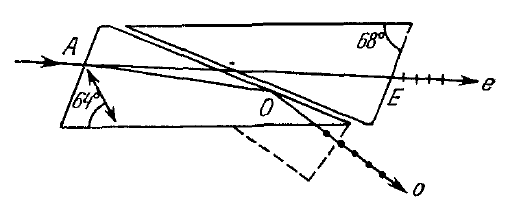
\includegraphics[scale=1]{nicole.png}
    \caption{Призма Николя}
    \label{fig:my_label}
\end{figure} 

На рисунке показано сечение призмы Николя плоскостью главного сечения. Двойная стрелка, наклоненная под углом $64^o$ к длинному ребру, указывает направление оптической оси. Такое обозначение применяется в дальнейшем и для других призм. Луч света, падая на искусственное основание кристалла, разделяется внутри кристалла на обыкновенный $AO$ и необыкновенный $AE$. Показатель преломления канадского бальзама $(n = 1,55)$ имеет промежуточное значение между обыкновенным $(n_o = 1,658)$ и необыкновенным $(n_e = 1,486) $ показателем преломления исландского шпата. Углы в призме Николя рассчитаны так, чтобы необыкновенный луч прошел через слой канадского бальзама, а обыкновенный претерпел на нем полное отражение и поглотился зачерненной боковой гранью. В результате свет, вышедший из призмы, окажется линейно поляризованным.

Призма Николя имеет скошенное основание, что вызывает параллельное боковое смещение падающего луча при прохождении его через призму. Следствием этого является кругообразное перемещение выходящего луча при вращении призмы вокруг ее оси. От этого недостатка избавлена призма Глана, имеющая форму прямоугольного параллелепипеда.

\begin{figure}[h!]
    \centering
    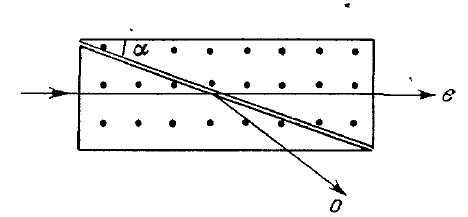
\includegraphics[scale=1]{glan.png}
    \caption{Призма Глана}
    \label{fig:my_label}
\end{figure} 

\newpage

\subsection{Призма Волластона}

Призма Волластона является одной из двулучевых поляризационных призм.  Призма состоит из комбинации стеклянной призмы с кристаллической из исландского шпата, оптическая ось которой параллельна преломляющему ребрую Призмы соприкасаются и склеиваются, как показано на рисунке. Показатель преломления стекла почти точно совпадает с показателем преломления исландского шпата. Падающий пучок неполяризованного света в призме разделяется на обыкновенный и необыкновенный. Выходящие лучи линейно поляризованного света отклоняются в разные стороны.

\begin{figure}[h!]
    \centering
    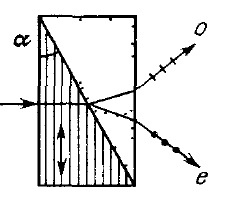
\includegraphics[scale=1]{volastone.png}
    \caption{Призма Волластона}
    \label{fig:my_label}
\end{figure} 

\subsection{Дихроичные пластинки}

У многих кристаллов поглощение света зависит от направления электрического вектора в световой волне. Это являние используется для получения линейно поляризованного света в дихроичных пластинках. К ним относятся, например, пластинки турмалина и поляроиды. В турмалине обыкновенный луч поглощается сильнее необыкновенного. Поэтому после прохождения через пластинку турмалина естественный свет становится частично поляризованным в плоскости главного сечения. Если пластинка достаточно толстая (около 1 мм), то в области видимого света обыкновенный луч поглощается практически полностью, так что прошедший свет окажется полностью линейно поляризованным. 


\subsection{Поляроиды}


Поляроиды применяются для получения линейно поляризованного излучения. Поляроиды обладают разрешенным направлением $P$ таким, что если вектор напряженности электрического поля световой волны $E$ параллелен этой оси, то эта волна свободно, практически без поглощения, проходит через поляроид. Если же $E \perp P$, то данная волна сильно поглощается веществом.

Таким образом, ставя на пути неполяризованного светового пучка поляроид П, мы получаем на выходе свет преимущественно с линейной поляризацией.

Действие поляроидов основано на линейном дихроизме, связанном с дихроизмом кристаллов или молекул полимера, внедренных в прозрачную матрицу и пространственно однородно ориентированных в ней. Например, кристаллы турмалина обладают дихроизмом: в видимом диапазоне света они преимущественно поглощают свет с поляризацией, перпендикулярной их оптической оси.
\newpage


\begin{figure}[h!]
    \centering
    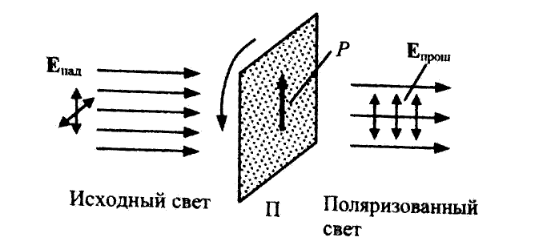
\includegraphics[scale=1]{polar.png}
    \label{fig:my_label}
\end{figure} 
Пусть на поляризатор падает частично поляризованный свет. Меняя ориентацию поляроида, находим, когда наблюдаются максимальная и минимальная интенсивности проходящего излучения.

Допустим, что свет содержит неполяризованную компоненту (естественный свет) и компоненту с линейной поляризацией. Если поляроид идеальный, то он "отсекает" половину интенсивности естественного света, поскольку все полярищации в нем представлены с равным весом. В то же время линейно поляризованная компонента либо полностью пропускается, либо полностью задерживается в зависимости от ориентации оси поляроида. Соответственно находим

\begin{equation*}
    I_{max} = \frac{1}{2}I_{\text{ест}} + I_{\text{пол}}, \hspace{10px} I_{min} = \frac{1}{2}I_{\text{ест}}.
\end{equation*}

В результате степень поляризации исследуемого излучения определяется по формуле

\begin{equation*}
    P = \frac{I_{\text{пол}}}{I_{\text{пол}} + I_{\text{ест}}} = \frac{I_{max} - I_{min}}{I_{max} + I_{min}}.
\end{equation*}


	
	\newpage
	
	\section{ Вращение плоскости поляризации (оптическая активность). Искусственная анизотропия оптических свойств, индуцированная механической деформацией, электрическим (эффект Керра и Поккельса) и магнитным (эффект Коттона-Муттона) полями.}
	\subsection{Естественная оптическая активность}
	\textit{Явление преломления плоскости поляризации} заключается в том, что в плоско-параллельных слоях некоторых веществ линейно поляризованный свет поворачивает плоскость своей поляризации по мере прохождения слоя. Вещества, в которых такое явление наблюдается, называются \textit{естественно-оптически активными} (в противовес магнитной оптической активности, причиной которой так же служет магнитное поле). Характерная особеннность таких веществ заключается в том, что поворот плоскости поляризации в них всегда происходит в одном и том же направлении (которое принято определять с точки зрения наблюдателя смотрящего на приближающийся свет). По этому принципу оптически активные вещества разделяют на \textit{правовращающие} и \textit{левовращающие}. Направление в котором свет проходит через этот слой не важно, и в прямом и в обратном напрвлении свет поварачивается направо от соответствующего наблюдателя. Если после прохождения слоя свет отразился и вернулся к наблюдателю через этот же слой, то направление его плоскости поляризации таким образом будет исходным. Это свойство оптической активности называется \textit{дисимметрией}.  
	Био эмпирически установил, что угол поворота плоскости поляризации $\chi$ прямо пропорционален толщине пройденного слоя $\ell$:
	\begin{equation}
	\label{chi}
	\chi = \alpha \ell
	\end{equation}
	Коэффициент $\alpha$ зависит от свойств вещества, температуры и длины волны проходящего света, причём от последней он зависит приблизительно как от обратного квадрата (то есть альфа увеличивается с уменьшением длины волны).
	Рассмотрим волну (в смысле электрического поля) $\mathbf{E} = \binom{E_{x}}{E_{y}}$
	%Рассмотри две волны поляризованные по часовой и против часовой стрелки ($\circlearrowright$ и $\circlearrowleft$ соответственно).
	\begin{align*}
	E_{x} &= A\cos(\chi)\cos(\omega t - kz) & E_{y} &= A\sin(\chi)\cos(\omega t - kz)
	\end{align*}
	Пользуясь~(\ref{chi})
	\begin{align*}
	E_{x} &= A\cos(-\alpha z)\cos(\omega t - kz) & E_{y} &= A\sin(-\alpha z)\cos(\omega t - kz)  
	\end{align*}
	Откуда
	\begin{gather}
	E_{x} = \frac{A}{2}\cos(\omega t - kz + \alpha z) + \frac{A}{2}\cos(\omega t - kz - \alpha z)\\
	E_{y} = \frac{A}{2}\cos\left(\omega t - kz + \alpha z + \frac{\pi}{2}\right) + \frac{A}{2}\cos\left(\omega t - kz - \alpha z - \frac{\pi}{2}\right)
	\end{gather}
	Введём новые обзначения
	\begin{align*}
	k^{\circlearrowright} &= k - \alpha & k^{\circlearrowleft} &= k + \alpha\\
	E_{x}^{\circlearrowright} &= \frac{A}{2}\cos(\omega t - k^{\circlearrowright} z) & E_{y}^{\circlearrowright} &= \frac{A}{2}\cos\left( \omega t - k^{\circlearrowright} z + \frac{\pi}{2}\right) \\
	E_{x}^{\circlearrowleft} &= \frac{A}{2}\cos(\omega t - k^{\circlearrowleft} z) & E_{y}^{\circlearrowleft} &= \frac{A}{2}\cos\left( \omega t - k^{\circlearrowleft}  - \frac{\pi}{2}\right)
	\end{align*}
	\begin{equation*}
	\mathbf{E} = \mathbf{E}^{\circlearrowright} + \mathbf{E}^{\circlearrowleft} = \binom{E_{x}^{\circlearrowright}}{E_{y}^{\circlearrowright}} + \binom{E_{x}^{\circlearrowleft}}{E_{y}^{\circlearrowleft}} 
	\end{equation*}
	Таким образом волна $\mathbf{E}$ раскладывается на две поляризованных по кругу в противоположных направлениях.
	Скорости этих волн:
	\begin{align*}
	v^{\circlearrowright} &= \frac{\omega}{k - \alpha} & v^{\circlearrowleft} &= \frac{\omega}{k + \alpha}
	\end{align*}
	Показатели преломления:
	\begin{align*}
	n^{\circlearrowright} &= \frac{c}{v^{\circlearrowright}} = \frac{c(k - \alpha)}{\omega} & n^{\circlearrowleft} &= \frac{c}{v^{\circlearrowleft}} = \frac{c(k + \alpha)}{\omega}
	\end{align*}
	\begin{equation}
	\label{alpha}
	\alpha = \frac{\omega}{2c}\left(n^{\circlearrowleft} - 	n^{\circlearrowright}  \right) 
	\end{equation}
	Пользуясь~(\ref{alpha}) если $\alpha > 0 $ то вращение плоскости поляризации происходит вправо, если  $\alpha < 0 $ -- влево.
	Френель показал эти соотношения опытно, позднее эти же соображения были полученны из уравнений Максвелла для материальной среды. 
	\subsection{Двойное лучепреломление}
	Явление разделения кинематической волны на две поляризованных по кругу при вращении плоскости поляризации называется \textit{круговым двойным лучепреломлением}. В общем случае двойное лучепреломление -- эффект расщепления в анизотропных средах луча света на две составляющие. Если луч света падает перпендикулярно к поверхности кристалла, то на этой поверхности он расщепляется на два луча. Первый луч продолжает распространяться прямо, и называется обыкновенным (o — ordinary), второй же отклоняется в сторону, и называется необыкновенным (e — extraordinary), причём обыкновенный и необыкновенный лучи поляризованы по-разному.
	\subsection{Искусственная анизотропия оптических свойств, индуцированная механической деформацией}
	Двойное лучепреломление можно наблюдать и в изотропных средах (аморфных телах), если подвергнуть их механическим нагрузкам.
	
	Изотропное тело, подвергнутое упругим деформациям, может стать анизотропным и изменить состояние поляризации проходящего света. Это явление носит название фотоупругости или пьезооптического эффекта. При одностороннем растяжении или сжатии тело становится подобным одноосному кристаллу с оптической осью, параллельной направлению приложенной силы. Мерой возникающей при этом оптической анизотропии служит разность показателей преломления обыкновенного и необыкновенного лучей. Опыт показывает, что эта разность пропорциональна напряжению $\sigma = \frac{\mathrm{d}F}{\mathrm{d}S}$  в данной точке тела. От этого напряжения будет зависеть разность показателей преломления:  $n_{o} - n_{e} = k\sigma$  ,  где $k$ – коэффициент пропорциональности, зависящий от свойств вещества.
	
	Поместим стеклянную пластинку $G$ между двумя поляризаторами $P_{1}$ и $P_{2}$ (рис.~\ref{mech}).
	\begin{figure}[H]
		\centering
		\begin{tikzpicture}[>=latex']
		\draw[red,->] (-3,0) -- (-2.5,0);
		\draw[red] (-3,0) -- (-2,0);
		\filldraw[fill=gray!22!white, draw=black] (-2,-0.5) -- (-2,0.5) -- (-1.5,0.5) -- (-1.5,-0.5) -- cycle node[below]{$P_{1}$};
		\draw[blue] (-2,0.5) -- (-1.5,-0.5);
		\draw[red] (-2,0) -- (-0.5,0);
		\draw[red,->] (-1.5,0) -- (-1,0);
		\filldraw[fill=blue!11!white, draw=black] (-0.5, -0.5) -- (-0.5, 0.5) -- (0.5, 0.5) -- (0.5, -0.5) -- cycle node[below]{$G$};
		\draw[->] (0,-0.75) -- (0,-0.5) node[near start, right]{\scriptsize $\vec{F}$};
		\draw[->] (0,0.75) -- (0,0.5) node[near start, right]{\scriptsize $\vec{F}$};
		\draw[red, ->] (0.5,0) -- (1,0);
		\filldraw[fill=gray!22!white, draw=black] (2,-0.5) -- (2,0.5) -- (1.5,0.5) -- (1.5,-0.5) -- cycle node[below]{$P_{2}$};
		\draw[blue] (2,0.5) -- (1.5,-0.5);
		\draw[red] (-3,0) -- (3,0);
		\draw[red,->] (2,0) -- (2.5,0);
		\end{tikzpicture}
		\caption{Искусственная анизотропия оптических свойств, индуцированная механической деформацией}
		\label{mech}
	\end{figure}
	 В отсутствие механической деформации свет через них проходить не будет. Если же стекло подвергнуть деформации, то свет может пройти, причем картина на экране получится цветная. По распределению цветных полос можно судить о распределении напряжений в стеклянной пластинке.
	\subsection{Эффект Керра и Поккельса}
	Под воздействием внешнего постоянного или переменного электрического поля в среде может наблюдаться двойное лучепреломление, вследствие изменения поляризации вещества. Пусть коэффициент преломления для обыкновенного луча равен $ n_{o}$, а для необыкновенного — $n_{e}$. Разложим разность коэффициентов преломления $n_{o} - n_{e}$, как функцию внешнего поля $E$, по степеням $E$. Если до наложения поля среда была неполяризованной и изотропной, то $n_{o}-n_{e}$ должно быть чётной функцией $E$ (при изменении направления поля эффект не должен менять знак). Значит, в разложении по степеням $E$ должны присутствовать члены лишь чётных порядков, начиная с $E^{2}$. В слабых полях членами высших порядков можно пренебречь, в результате чего
	\begin{equation}
	n_{e}-n_{o} \sim k{E}^{2}
	\end{equation}
	Эффект Керра обусловлен, главным образом, гиперполяризуемостью среды, происходящей в результате деформации электронных орбиталей атомов или молекул или вследствие переориентации последних.
	\subsection{Эффект Коттона-Муттона}Эффект Коттона — Мутона, двойное лучепреломление света в изотропном веществе, помещенном в поперечное магнитное поле (перпендикулярное световому лучу). Впервые обнаружено в коллоидных растворах Дж. Керром и (независимо от него) итальянским физиком К. Майораной в 1901. Подробно исследовано Эме Коттоном (Aime Cotton) и А. Мутоном (Н. Mouton) B 1907. Для наблюдения К.— М. э. через образец прозрачного изотропного вещества, помещенный между полюсами сильного электромагнита, пропускают монохроматический свет, линейно поляризованный в плоскости, составляющей с направлением магнитного поля угол $\frac{\pi}{4}$. В магнитном поле вещество становится оптически анизотропным (его оптическая ось параллельна магнитному полю $Н$), а проходящий свет превращается в эллиптически поляризованный, т. к. он распространяется в веществе в виде 2 волн — обыкновенной и необыкновенной, имеющих разные фазовые скорости. Разность показателей преломления обыкновенного $n_{o}$ и необыкновенного $n_{e}$ лучей, называемая величиной двойного лучепреломления, равна:
	$$n_{e} - n_{o} = kH^{2}\lambda,$$
	где Н — напряжённость магнитного поля, $k$ — зависящая от вещества константа, называемая постоянной Коттона—Мутона, $\lambda$ — длина волны света. Величина С обратно пропорциональна абсолютной температуре $Т$ и, как правило, очень мала. 
	
	\newpage
	
	\section{Принцип суперпозиции и интерференция монохроматических волн. Интерференция плоской и сферической волн. Видность полос.}

\theornp{Принцип суперпозиции}{Если в одной точке пространства накладываются колебания двух волн, то они порождают новую волну, равную их векторной сумме.}

Из-за наличия принципа суперпозиции возможно явление интерференции, когда волны взаимно усиляют друг друга, или же наоборот, гасят.

\Def{Монохроматическая волна} --- волна, в спектр которой входит только одна частота.

\subsection{Интерференция двух плоских монохроматических волн. Ширина полосы}

Рассмотрим сперва интерференцию двух плоских монохроматических волн. Пусть распространяются две волны с одинаковой частотой $\omega$:

\begin{align*}
	E_1 &= a_1 e^{i(\vec{k}\cdot \vec{r}_1 - \phi_1)} \cdot e^{-i\omega t}\\
	E_2 &= a_2 e^{i(\vec{k}\cdot \vec{r}_2 - \phi_2)} \cdot e^{-i\omega t}
\end{align*}

Как мы знаем, сами по себе волны складываются. Посмотрим теперь за интенсивностью $I$, которую мы запишем как $I = E E^*$. Распишем суммарную интенсивность (принимаем во внимание, что временная часть в экспоненте одинаковая у всех, поэтому она сократится при произведении с комплексно сопряженным и поэтому следить за ней не будем):

\begin{align*}
	I_{\sum} = (E_1 + E_2) (E_1 + E_2)^* = E_1 E_1^* + E_1 E_2^* + E_2 E_1^* + E_2 E_2^* = \\
	= a_1^2 + 2 a_1 a_2 \cos(k \Delta - \Delta\phi) + a_2^2 = I_1 + I_2 + 2 \sqrt{I_1 I_2} \cos(k \Delta - \Delta\phi)
\end{align*}

Здесь мы ввели $\Delta = r_2 - r_1$, $\Delta\phi = \phi_2 - \phi_1$. Напоминаю, что $k = 2\pi / \lambda$.

\textit{Если же $k_1 \ne k_2$, то вместо $k$ в результирующей формуле будет $K = |k_1 - k_2|$.}

\subsubsection{Ширина полосы}

Рассмотрим чуть более общий случай, когда $|k_1| = |k_2|$, но при этом волны сходятся под некоторым углом $\alpha$. Тогда $K = 2 k \sin(\alpha/2)$

\textbf{Шириной полосы} будем называть расстояние между ближайшими максимумами (\textit{вообще говоря, в МФТИшном конспекте написано что между минимумами, а между максимумами это расстояние между полосами, но наш лектор видимо так не считает, но строго говоря какая разница казалось бы}). В нашем случае она оказывается равной:

\begin{equation*}
	\Delta x = \frac{2\pi}{K} = \frac{2 \pi}{2 k \sin(\alpha/2)} = \frac{\lambda}{2\sin(\alpha/2)} \approx \frac{\lambda}{\alpha}
\end{equation*}

\subsection{Интерференция плоской и сферической монохроматических волн}

Внимание на картинку.

\begin{figure}[H]
	\centering
	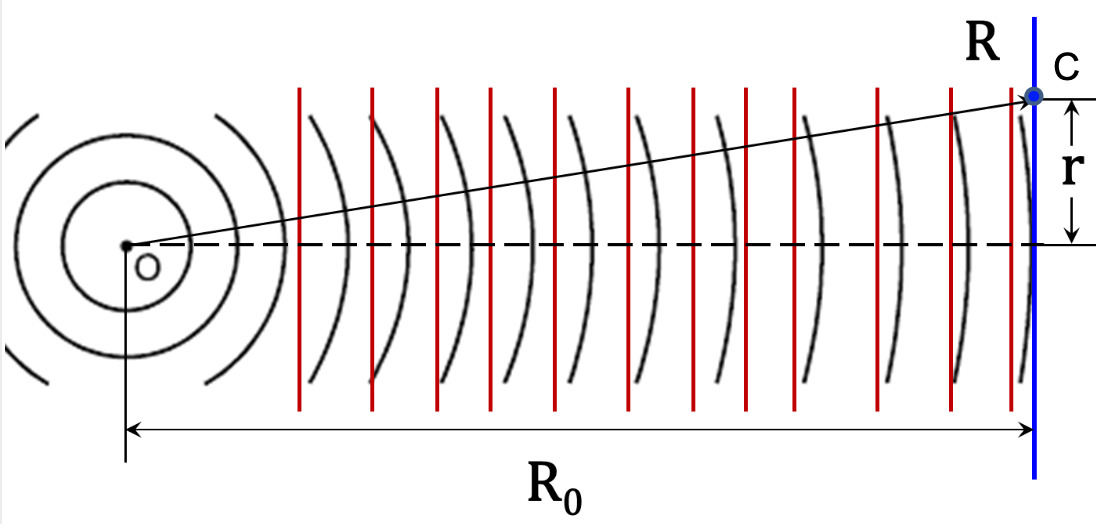
\includegraphics[width=\textwidth]{16_1}
\end{figure}

Будем рассматривать область, где $R_0 \gg r$. При этом:

\begin{equation*}
	R = \sqrt{R_0 + r^2} \approx R_0 + \frac{r^2}{2R_0}
\end{equation*}

Для сферической волны:

\begin{equation*}
	E_{sp} = \frac{a_1}{R_0} e^{i k r} e^{-i \omega t} \approx \frac{a_1}{R_0} e^{i k (R_0 + r^2 / (2 R_0))} e^{-i \omega t}
\end{equation*}

Для плоской волны:

\begin{equation*}
	E_{f} = a_2 e^{i k R_0  - i \omega t}
\end{equation*}

Если это счастье расписать так же, как мы делали с плоской волной, то получим:

\begin{equation*}
	I_{\sum} = \frac{a_1^2}{R_0^2} + a_2^2  + 2 \frac{a_1 a_2}{R_0} \cos \left(k \frac{r^2}{2 R_0}\right)
\end{equation*}

\subsection{Видность}

Для характеристики выраженности интерференции вводят величину, называемую \textbf{видностью} $V$:

\begin{equation}
	V = \frac{I_{max} - I_{min}}{I_{max} + I_{min}}
	\label{eq:Vidnost}
\end{equation}

где $I_{max}$, $I_{min}$ --- максимальное и минимальное значения интенсивности в области интерференции волн.

При интерференции двух \textbf{монохроматических} волн видность будет равна:

\begin{equation*}
	V = \frac{2 \sqrt{I_1 I_2}}{I_1 + I_2}
\end{equation*}
	
	\newpage
	
	
	\section{Понятие о когерентности. Частично когерентный свет. Основные интерференционные
		схемы. Интерференция плоских волн, пространственный период полос.}
	Монохроматических волн не бывает в природе. В реальности волны часто излучаются модулированными как по амплитуде, так и по частоте. Такие называют квазимонохроматическими. 
	\begin{align*}
	a(t) \cos (\omega t + b(t))
	\end{align*}
	\textbf{когерентными наз ывают две волны, если у них постоянная разность фаз}\\
	Так две монохроматические волны когерентны, если у них одинаковая частота.\\
	Если есть какая-то маленькая разница в частотах $\Delta \omega$ то говорят о времени когерентности $t \Delta \omega \sim \pi$. Предполагаю малость $\Delta \omega$ получаем $t \sim \dfrac{\lambda^2}{2c \Delta \lambda}$ отсюда получается то, что называют длинной когерентности $l \sim \dfrac{\lambda^2}{2\Delta \lambda}$\\
	Пусть у нас есть две плоские волны. 
	\begin{align*}
	A_1 = a_1 \cos \mathbf{k_1 r} - \omega t + \phi_1\\
		A_2 = a_2 \cos \mathbf{k_2 r} - \omega t + \phi_2
	\end{align*}
	Тогда не сложно их сложить и получить распределение интенсивности
	\begin{align*}
	I = I_1 + I_2 + 2\sqrt{I_1 I_2} \cos( \mathbf{(k_1 - k_2)r} + \phi_1 - \phi_2 )
	\end{align*}
	Ага, теперь мы знаем, что интенсивность постоянна в плоскостях перпендикулярных $\mathbf{k_1 - k_2}$ \\
	Расстояние между плоскостями максимумов будет $\dfrac{2\pi}{|\mathbf{k_1 - k_2}|}$. Для равных по модулю векторов $\dfrac{\lambda}{2 \sin \alpha/2}$ где альфа это угол между векторами\\
	\subsection{Основные схемы}
	\textbf{Схема Юнга.} 
	\begin{figure}[h]
		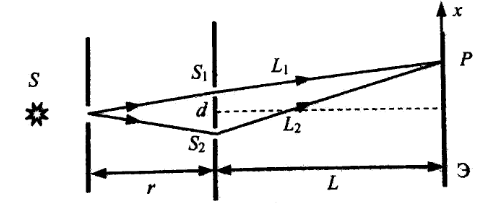
\includegraphics[scale = 0.7]{17_1}
	\end{figure}
	Ширина полос и расстояние между ними равно $\dfrac{\lambda L}{d}$\\ 
	\textbf{Тонкий клин.} В приближении малых углов падения и малости угла альфа просто поворачивает входной луч на $(n-1)\alpha$\newpage
	\begin{figure}[h]
		\centering
		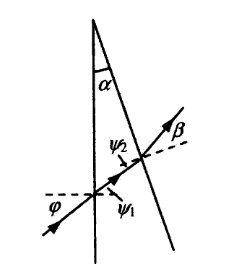
\includegraphics[scale = 0.7]{17_2}
	\end{figure}
	\textbf{Бипризма Френеля} Две призмы из прошлого пункта. В итоге получаем, что эффективно один источник расслаивается на два. Расстояние между ними $2a(n-1)\alpha$, и теперь задача свелась просто к опыту Юнга \\
	\begin{figure}[H]
		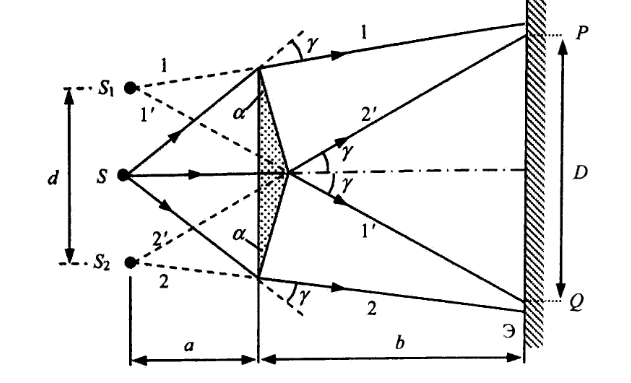
\includegraphics[scale = 0.5]{17_3}
	\end{figure}

	
	\newpage
	
	\section{Интерференция волн от одного источника. Интерференционные опыты с делением волнового фронта (опыт Поля, бипризма Френеля, зеркала Френеля, билинза Бийе, зеркало Ллойда). Схема Юнга.}

\subsection{Интерференция волн от одного источника}


Для наблюдения интерференции света необходимо:
\begin{flushleft}
Постоянство во времени разности фаз складываемых колебаний


Равенство частот интерферирующих волн


Параллельность векторов \textbf{$E_1$} и \textbf{$E_2$}


Независимость от времени амплитуд световых волн.
\end{flushleft}

Если разность фаз двух колебаний с течением времени изменяется очень медленно, то говорят, что колебания остаются временно когерентными. \\ \\
Обозначим за $\tau$ время, за которое разность фаз двух колебаний успела измениться на величину, сравнимую $\pi$.\\ \\ За это время волна распространится на расстояние $c \tau$ , и колебания напряженности электрического поля волны в точках, удалённых друг от друга на это расстояние вдоль направления распространения волны оказываются некогерентными.\\ \\ Таким образом, расстояние вдоль направления распространения плоской волны, на котором случайные изменения разности фаз колебаний достигают величины, сравнимой с $\pi$, называют длиной когерентности (расстояние, при прохождении которого две или несколько волн утрачивают когерентность.)\\ \\

Наиболее распространённым способом получения двух когерентных волн является расщепление волны, излучаемой одним источником, на две волны, распространяющиеся по разным путям, но, в конце концов, встречающиеся в одной точке, где и происходит их сложение. Если запаздывание одной волны по отношению к другой, связанное с разностью пройденных ими путей, меньше длины когерентности, то колебания в точке сложения будут когерентными, и будет наблюдаться явление интерференции. Когда разность оптических путей двух волн приближается к длине когерентности, интерференционная картина исчезает, и интенсивность в каждой точке пространства становится равной сумме интенсивностей двух волн.

\subsection{Методы получения когерентных пучков}

Существующие экспериментальные методы получения когерентных пучков из одного светового пучка можно разделить на два класса.
\\ \\
В \textbf{методе деления волнового фронта} пучок пропускается, например, через два близко расположенных отверстия в непрозрачном экране.Такой метод пригоден лишь при достаточно малых размерах источника.
\\ \\
 В другом методе пучок делится на одной или нескольких частично отражающих, частично пропускающих поверхностях. Этот \textbf{метод деления амплитуды} может применяться и при протяженных источниках. Он обеспечивает большую интенсивность и лежит в основе действия разнообразных интерферометров. В зависимости от числа интерферирующих пучков различают двулучевые и многолучевые интерферометры. \\ \\ 
 
 \subsection{Схема Юнга}

\begin{center}
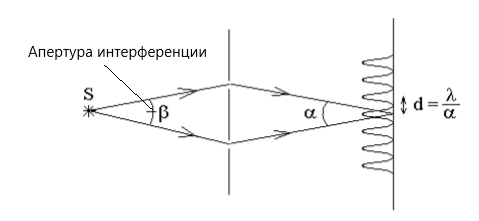
\includegraphics[scale = 0.7]{Yung}
\end{center}

Свет падает на экран с узкой щелью, дальше его можно рассматривать как точечный, монохроматический источника света $S$. После дифракции на щели световая волна распространялась до двух маленьких отверстий $S_1$ и $S_2$, сделанных в экране. После очередной дифракции два расходящихся пучка света перекрывают друг друга, и, являясь когерентными, при наложении дают интерференционную картину.

\subsection{Опыт Поля}

Опыт Поля - способ наблюдения интерференции света основанный на методу деления амплитуды.\\

В опыте Поля свет от источника S отражается двумя поверхностями тонкой прозрачной плоскопараллельной пластинки, в любую точку P, находящуюся с той же стороны от пластинки, что и источник, приходят два луча. Эти лучи образуют интерференционную картину. Для определения вида полос можно представить себе, что лучи выходят из мнимых изображений S1 и S2 источника S, создаваемых поверхностями пластинки. На удаленном экране, расположенном параллельно пластинке, интерференционные полосы имеют вид концентрических колец с центрами на перпендикуляре к пластинке, проходящем через источник S

\begin{center}
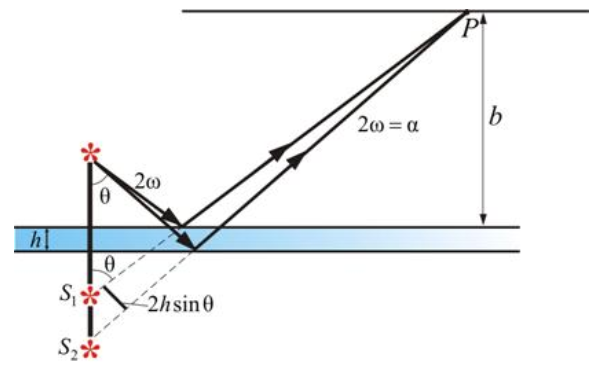
\includegraphics[scale = 0.5]{Pol}
\end{center}

\subsection{Бипризма Френеля}

Бипризма Френеля - призма, в основании которой находится тупоугольный равнобедренный треугольник.

\begin{center}
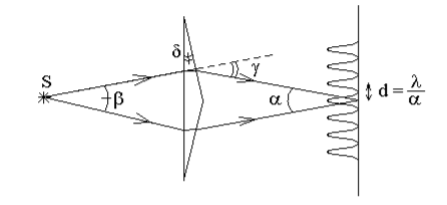
\includegraphics[scale = 0.5]{Biprizma}
\end{center}

Угол $\delta$ при основании треугольника и угол $\gamma$ , на который каждый из двух тонких оптических клиньев поворачивает луч, связаны соотношением:

$$\gamma = (n-1) \delta$$

\subsection{Зеркала Френеля}

Две когерентные световые волны получаются в результате отражения от двух зеркал $M$ и $N$, плоскости которых наклонены под небольшим углом $\phi$ друг к другу:
\begin{center}
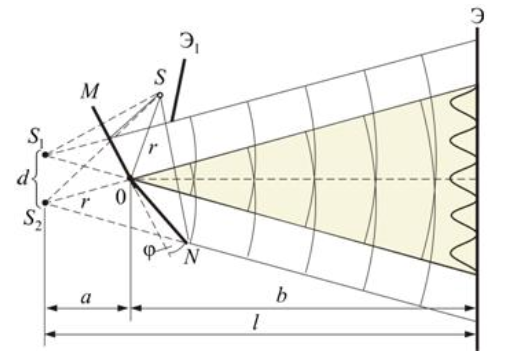
\includegraphics[scale = 0.5]{Zerkala}
\end{center}
Источником служит узкая ярко освещенная щель $S$, параллельная ребру между зеркалами. Отраженные от зеркал пучки падают на экран, и в той области, где они перекрываются (поле интерференции), возникает интерференционная картина. От прямого попадания лучей от источника $S$ экран защищен ширмой Э. Для расчета освещенности $J$ экрана можно считать, что интерферирующие волны испускаются вторичными источниками $S_1$   и  $S_2$, представляющими собой мнимые изображения щели $S$ в зеркалах. Поэтому $J$ будет определяться формулой двулучевой интерференции, в которой расстояние $l$ от источников до экрана следует заменить на  $a+b$ , где  $a \approx r$ - расстояние от S до ребра зеркал, $b$ - расстояние от ребра до экрана. Расстояние $d$ между вторичными источниками равно: $d \approx 2 a \phi$ . Поэтому ширина интерференционной полосы на экране равна:
$$ \Delta x \approx \frac{\lambda l}{d} = \frac{\lambda(a+b)}{2a \phi}$$

\subsection{Билинза Бийе}

Из обычной линзы вырезают полоску, получается билинза Бийе:

\begin{center}
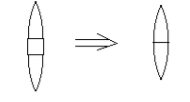
\includegraphics[scale = 0.5]{Bilinza1}
\end{center}

Точку пересечения фокальной плоскости и оси симметрии задачи можно назвать фокусом билинзы Бийе. Рассмотрим точечный источник света $S$, расположенный в фокусе билинзы Бийе и рассмотрим лучи света проходящие через верхнюю половину билинзы:

\begin{center}
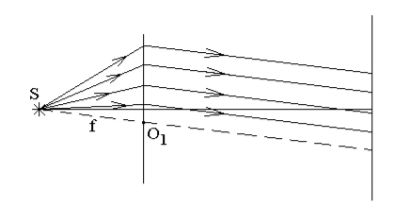
\includegraphics[scale = 0.5]{Bilinza2}
\end{center}

Если  верхнюю  половину  билинзы  достроить  вниз  до  полной  линзы,  то центр  полной  линзы  будет  находиться  в  некоторой  точке $O_1$,  расположенной ниже оси симметрии задачи.       Лучи,  прошедшие  через  верхнюю  половину  билинзы,  после  билинзы пойдут параллельно прямой $SO_1$, так как луч, проходящий через центр линзы $O_1$, должен пройти линзу без изменения направления. Остальные лучи обязаны быть параллельными лучу $SO_1$, так как источник света находится в фокальной плоскости. Как видно из рисунка этот пучок лучей наклонен вниз относительно оси симметрии задачи.       Аналогично, лучи, прошедшие нижнюю половину билинзы, пойдут после билинзы параллельным пучком лучей слегка наклоненным вверх.       На  экран  приходят  два  параллельных  пучка  лучей,  представляющих собой  две  плоских  волны.  Интерференционные  полосы  будут  иметь одинаковую ширину по всему экрану, так как угол между интерферирующими лучами в каждой точке экрана один и тот же.

\subsection{Зеркало Ллойда}

Интерферируют два луча, один идет прямо от источника света $S$ к экрану, второй отражается от зеркала, здесь $\beta$ - апертура интерференции. Ширина полос $ d = \frac{\lambda}{\alpha}$
\begin{center}
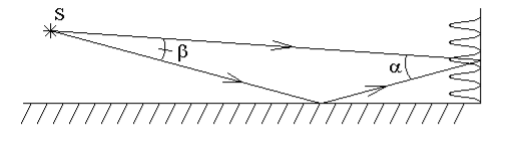
\includegraphics[scale = 0.5]{Loyd}
\end{center}
В нижней точке, где экран соприкасается с зеркалом, находится середина темной полосы. В эту точку волны приходят в противофазе, так как при отражении от зеркала одна из волн теряет половину волны.
	
	\newpage
	
	

\section{Временная когерентность. Интерференция немонохроматических волн. Время и длина когерентности. Соотношения между временем когерентности и шириной спектрального интервала.}
\subsection{Интерференция немонохроматических волн}
\subsubsection{Корегентность}

Две волны называются \textit{когерентными}, если разность их фаз является постоянной. Когерентными являются две монохроматические волны, если только они имеют одинаковые частоты.

Если разность фаз волн меняется со временем, то эти волны называются \textit{некогерентными}.
\subsubsection{Время и длина когерентности}

Рассмотрим сложение двух волн с разными частотами $\omega_1$ и $\omega_2$.

Временем когерентности называется такое время, в течение которого разность фаз рассматриваемых волн меняется незначительно. В случае двух волн

\begin{equation*}
    A_1 = a_1 \cos(\omega_1 t + \alpha_1)
\end{equation*}

\begin{equation*}
    A_2 = a_2 \cos(\omega_2 t + \alpha_2)
\end{equation*}

разность фаз равна

\begin{equation*}
    \Delta \phi = \Delta \omega \cdot t + \Delta \alpha, \Delta \omega = \omega_1 - \omega_2, \Delta \alpha = \alpha_1 - \alpha_2
\end{equation*}

Когда сдвиг фаз составит $\Delta \omega \cdot t \sim \pi$, волны уже нельзя считать когерентными. Поэтому время когерентности определяется условием

\begin{equation*}
    \Delta \phi(t+t_{\text{ког}} - \Delta \phi(t) \sim \pi
\end{equation*}

\begin{equation*}
    t_{\text{ког}} \sim \frac{\pi}{\Delta \omega}
\end{equation*}

Переходя от частоты к длине волны по формуле $\omega = \frac{2\pi c}{\lambda}$ и считая $\Delta \omega \ll \omega$ , получим

\begin{equation*}
    t_{\text{ког}} \sim \frac{\lambda^2}{2c\Delta \lambda}
\end{equation*}


Длина когерентности - путь, проходимый волнами за время когерентности. Она составляет



\begin{equation*}
    l_{\text{ког}} = c t_{\text{ког}} \sim \frac{\lambda ^2}{2\Delta \lambda}
\end{equation*}

\subsubsection{Связь времени когерентности с шириной спектра}

Представим волновой пакет в виде суперпозиции монохроматических волн:

\begin{equation*}
    A(t) = \int_{-\infty}^{\infty} a(\omega)e^{-i\omega t} \frac{d\omega}{2\pi},\hspace{10px} a(\omega) = \int_{-\infty}^{\infty} A(t)e^{i\omega t}dt 
\end{equation*}


Пусть фурье-спектр сигнала дается выражением
\begin{equation*}
    a(\omega) = \begin{cases}
   a_0, |\omega-\omega_0| < \frac{\Delta \omega}{2}, \\
   0, |\omega-\omega_0| > \frac{\Delta \omega}{2}.
 \end{cases}
\end{equation*}

Соответствующая временная зависимость сигнала определится по первой формуле:

\begin{equation*}
    A(t) = \int_{-\infty}^{\infty} a(\omega)e^{-i\omega t} \frac{d\omega}{2\pi},\hspace{10px} \frac{a_0}{2\pi}\int_{\omega_0-\Delta\omega/2}^{\omega_0-\Delta\omega/2}e^{-i\omega t} d\omega = a_0 e^{-i\omega_0 t} F(t),
 \end{equation*}   
    
Здесь введена функция
\begin{equation*}
    F(t) = \frac{1}{2\pi it }\left(e^{i\Delta\omega t/2} - e^{-i\Delta\omega t/2}\right) = F_m\frac{\sin(\Delta\omega\cdot t/2)}{(\Delta\omega\cdot t/2)},
\end{equation*}

где $F_m(t) = \frac{\Delta \omega}{2\pi}$.

\medskip

Функция $F(t)$ обращается в первый раз в нуль при $\frac{\Delta \omega \cdot t}{2} = \pi$,  то есть в момент времени

\begin{equation*}
    t = \tau = \frac{2\pi}{\Delta \omega}.
\end{equation*}

Эта величина есть характерное время существования волнового пакета - время когерентности.
\subsection{Влияние немонохроматичности на наблюдаемое число интерференцционных полос}

Сигнал называется квазимонозроматическим, если его можно представить в виде

\begin{equation*}
    A(t) = a(t)\cos(\omega_0t+\phi(t)),
\end{equation*}


где амплитуда a(t) и фаза $\phi(t)$ - медленно меняющиеся функции.

\bigskip

Можно наблюдать интерференционную картину от квазимонозроматического источника. Действительно, свет, испускаемый таким источником, представляет собой суперпозицию монохроматических волн. Каждую из них можно расщепить на две волны(например, с помощью схемы Юнга), тогда получаемая в конце пара когерентных волн уже создает интерференционную картину.

Интерференционная каартина от всего спектра получается наложением интерференционных картин от отдельных компонент спектра. Однако, период отдельных картин зависит от соответствующей длины волны, поэтому положение максимумов и минимумов различно для разных компонент спектра. Это ограничивает общее число наблюдаемых полос от источника.

\bigskip

Рассмотрим компоненту спектра с длиной волны $\lambda$. Разность хода в опыте Юнга составляет
\begin{equation*}
    \delta \approx \frac{xd}{L}
\end{equation*}

Максимумы интерференционной картины наблюдаются в точках, для которыз $\delta = m\lambda$

\begin{equation*}
    x_m^{(max)} = \frac{\lambda L}{d}m.
\end{equation*}

Таким рьпащрм, ширина интерференционной полосы равна

\begin{equation*}
    \Delta x = \frac{\lambda L}{d}
\end{equation*}

Учтем, что источник создает немонохроматический свет в спектральном диапазоне $\Delta \lambda$. Для такого света длина когерентности есть

\begin{equation*}
    l_{\text{ког}} \sim \frac{\lambda^2}{\Delta \lambda}.
\end{equation*}

Максимальная разность хода лучей $\delta$, при которой они еще могут считаться когерентными, не должна превышать $l_{\text{ког}}$:

\begin{equation*}
    \delta < l_{\text{ког}}.
\end{equation*}

Отсюда наибольший порядок интерференции:

\begin{equation*}
    \delta_{max} = m_{max} \lambda \sim \frac{\lambda^2}{\Delta \lambda}  \Rightarrow m_{max} \sim \frac{\lambda}{\Delta\lambda}.
\end{equation*}

Тогда максимальное число наблюдаемых полос интерференции составляет

\begin{equation*}
    2m_{max}+1 \sim \frac{2\lambda}{\Delta\lambda}.
\end{equation*}


	
	\newpage
	
	\section{Временная когерентность. Видность интерференционной картины. Предельная разность хода и полное число наблюдаемых интерференционных полос.}
	\subsection{Степень когерентности}
		Рассмотрим квазимонохроматический свет, с фазово-амплитудной модуляцией:
		\begin{equation*}
		E(t) = a(t)e^{i\omega_{0} t} = a_{0}(t)e^{i\delta(t)}e^{i\omega_{0} t}
		\end{equation*}
		где $a_{0}(t)$ и $\delta(t)$ -- медленно меняющиеся функции времени. Для реального света эти функуции -- случайные.
	В предположении, что приёмники света ринимают только квадраты напряжённостей (интенсивности) световых полей, усреднённых по промежуткам времени, весьма большими с периодами колебаний квазимонохроматического света и временами изменения функций вышеописанных случайных функций. Световые потоки в срелнем будем полагать стационарными.
	Квадрат поля можно представить следующим образом:
	\begin{gather*}
	\big(\Re(E)\big)^{2} = \left( \frac{E + {E}^{*}}{2}\right)^{2} = \frac{E^{2} + {E}^{*2}}{4} + \frac{E\bar{E}}{2}\\
	E^{2} + E^{*2} = 2a_{0}^{2}\cos\big(2(\omega_{0}t + \delta) \big) \text{-- бысроосциллирующая величина,}\\ \text{при усреднении выпадет, откуда}\\
	\text{интенсивность полагается:} \ I = \overline{E{E}^{*}}
	\end{gather*}
	Пусть теперь в момент времени $t$ колебания приходят в точку $P$ из источников $S_{1}$ и $S_{2}$? из которых они вышли во времена $t - \theta_{1}$ и $t - \theta_{2}$ соответственно.
	Тогда
	\begin{equation*}
	E = E(P,t) = E_{1}(t - \theta_{1}) + E_{2}(t - \theta_{2})
	\end{equation*} 
	\begin{multline*}
	I = \overline{E_{1}(t - \theta_{1})\cdot E_{1}^{*}(t - \theta_{1})} + \overline{E_{2}(t - \theta_{2})\cdot E_{2}^{*}(t - \theta_{2})} + \\ + \overline{E_{1}(t - \theta_{1})\cdot E_{2}^{*}(t - \theta_{2}) + E_{2}(t - \theta_{2})\cdot E_{1}^{*}(t - \theta_{1})}
	\end{multline*}
	В силу предположения о средней стационарности потоков первое слагаемое не зависит от $t$ и $\theta$, обозначим его $I_{1}$. Пологая $\tau$ -- отрезком времени усреднения:
	\begin{equation*}
	I_{1} = \frac{1}{\tau} \int\limits_{-\frac{\tau}{2}}^{\frac{\tau}{2}} E_{1}(t - \theta_{1})\cdot E_{1}^{*}(t - \theta_{1}) \mathrm{d} t = \frac{1}{\tau} \int\limits_{-\frac{\tau}{2}}^{\frac{\tau}{2}} E_{1}(t)\cdot E_{1}^{*}(t) \mathrm{d} t
	\end{equation*}
	Аналогично второй член 
	\begin{equation*}
	I_{2} = \frac{1}{\tau} \int\limits_{-\frac{\tau}{2}}^{\frac{\tau}{2}} E_{2}(t)\cdot E_{2}^{*}(t) \mathrm{d} t
	\end{equation*}
	Последний перекрёсный член зависит таким образом только от $\theta = \theta_{2} - \theta_{1}$, его обозначают $F_{12}(\theta)$ и называют корреляционной функцией колебаний $E_{1}(t - \theta_{1}) $ и  $ E_{2}(t - \theta_{2})$. Если $E_{1}(\cdot)$ и  $E_{2}(\cdot)$ равнs функция называется автокорреляционной (для простоты $F(\theta)$).
	Функция
	$$f_{12}(\theta) = \frac{F_{12}(\theta)}{\sqrt{I_{1}I_{2}}}$$
	называется нормированной корреляционной. Через неё запишем интенсивность в $P$.
	$$I = I_{1} + I_{2} + 2\sqrt{I_{1}I_{2}}\Re\big(f_{12}(\theta)\big) $$
	Пользуясь квазимонохроматическим приближением $E_{i} = a_{i}e^{i\omega_{0}t}, \ i = 1,2$, так что
	\begin{equation*}
	\overline{a_{1}(t) a_{2}^{*}(t - \theta)}e^{i\omega t} = \sqrt{I_{1}I_{2}}f_{12}(\theta)
	\end{equation*}
	Функция 
	\begin{equation*}
	\gamma_{12}(\theta) = f_{12}(\theta)e^{-i\omega_{0} \theta}
	\end{equation*}
	называется комплексной степенью когерентности.
	\begin{gather*}
	I = I_{1} + I_{2} + 2\sqrt{I_{1}I_{2}}\Re\big(\gamma_{12}(\theta)e^{-i\omega_{0}t}\big) \\I = I_{1} + I_{2} + 2\sqrt{I_{1}I_{2}}|\gamma_{12}(\theta)|\cos(\omega_{0}\theta + \delta)
	\end{gather*}
	Тогда
	\begin{align}
	\label{maxmin}
	I_{max} &= I_{1} + I_{2} + 2\sqrt{I_{1}I_{2}}|\gamma_{12}(\theta)| & I_{min} = I_{1} + I_{2} - 2\sqrt{I_{1}I_{2}}|\gamma_{12}(\theta)|
	\end{align}
	\subsection{Видность интерференционной картины.}
	\begin{definition}
		Видностью интерференционной картины называется величина $V$, определяемая следующим образом:
		\begin{equation}
		V = \frac{I_{max} - I_{min}}{I_{max} + I _{min}},
		\end{equation}
		где $I_{max}$ и $I_{min}$ -- интенсивности света в точках максимума и минимума интерфенренции соответственно.
	\end{definition}
	Пользуясь~(\ref{maxmin}) 
	\begin{equation*}
	V = \frac{\sqrt{I_{1}I_{2}}}{I_{1} + I_{2}}|\gamma_{12}(\theta)|
	\end{equation*}
	Если $|\gamma_{12}(\theta)|$ при всех $\theta$ равна нулю, то $V = 0$ и интерференционныйй полосы не видны, колебания называются полностью некогерентными. Когда же $|\gamma_{12}(\theta)|$ при всех $\theta$ равна единие, то когеррентность называется полной. В остальных случаях говорят о частичной некогерентности.
	\subsection{Временная когерентность}
	\begin{wrapfigure}{r}{0.5\textwidth}
		\centering
		\begin{tikzpicture}[>=latex']
		\filldraw[fill=gray!22!white, draw=black] (-1,-1.5) -- (1,-1) -- (1,1.5) -- (-1,1) -- cycle;
		\draw[->] (-2.5,0.5) -- (-1.5,0);
		\draw[->] (-2.5,1.25) -- (-1.5,0.75);
		\draw[->] (-2.5,-0.25) -- (-1.5,-0.75);
		%
		\draw[->] (-1,2) -- (0,1.5);
		\draw[->] (-1.75,1.75) -- (-0.75,1.25);
		\filldraw[fill=white, draw=black] (0.5,-0.5) circle [x radius=0.15, y radius=0.1, rotate=25] node[below] {\scriptsize $Q_{2}$};
		\filldraw[fill=white, draw=black] (-0.5,0.5) circle [x radius=0.15, y radius=0.1, rotate=25] node[below] {\scriptsize $Q_{1}$};
		\draw[->]  (0.5,-0.5) -- (2,-1.5);
		\draw[->]  (-0.5,0.5) -- (2,-1.5);
		\node at (2.2,-1.7) {\scriptsize $P$};
		\end{tikzpicture}
		\caption{Излучение от двух отверстий}
		\label{shild} 
	\end{wrapfigure}
	Пусть рассматривается когерентность одного и того же светового поля в пространственно-временных точках $R_{1}(Q_{1},t_{1})$ и $R_{2}(Q_{2},t_{2})$. Пусть пространственные точки $Q_{1}$ и $Q_{2}$ являются маленькими отверстиями в непрозрачном экране на пути светового излучения, из этих отверстий выйдет дифрагмированный свет и пусть он придёт в удалённую точку $P$ одновременно (рис.~\ref{shild}).
	
	По определению колебания в $R_{1}(Q_{1},t_{1})$ и $R_{2}(Q_{2},t_{2})$ мы называем когерентными или некогерентными, если когерентны или некогерентны соответствующие колебания в $P$. Степень когерентности $\gamma(\theta)$ определяется для них  той же величиной, что и для $R_{1}(Q_{1},t_{1})$ и $R_{2}(Q_{2},t_{2})$.
	
	Если точки $Q_{1}$ и $Q_{2}$ совпадают, но свет попадает в $P$ разными путями, то $R_{1}(Q_{1},t_{1})$ и $R_{2}(Q_{2},t_{2})$ отличаются только $t_{1}$ и $t_{2}$. В этом случае говорят о \textit{временной когерентности}. При $t_{1} = t_{2}$ степень временной когерентности равна единице,  с увелечением  разности этих времён степень когерентности убыает. Максимальное значение $|t_{2} - t_{1}|$, при котором когерентность ещё сохраняется, называется временем когерентности. Расстояние $\ell = v|t_{2} - t_{1}|$, проходимое светом за это время, называется длинной когерентности.
	   \subsection{Предельная разность хода и полное число наблюдаемых интерференционных полос.}
	   Пусть спектральный интервал излучения, создающего наблюдаемую
	   интерференционную картину, ограничен длинами волн $\lambda$ и $\lambda + \Delta \lambda$.
	   Интерференционная картина будет размываться, если максимум m-го порядка
	   для длины волны $\lambda + \Delta \lambda$ будет накладываться на максимум
	   $(m + 1)$-го порядка для длины волны $\lambda$. Тогда с учетом условия максимума
	   \begin{equation*}
	   m_{max}(\lambda + \Delta\lambda) = (m_{max} + 1) \lambda 
	   \end{equation*}
	   Откуда
		\begin{equation}
		\boxed{m_{max} = \frac{\lambda}{\Delta \lambda}}
		\end{equation}   
		С другой стороны, интерференция наблюдается до тех пор, пока разность
		хода не превышает длину когерентности $\ell$:
		\begin{equation*}
		\ell \approx m_{max}\cdot \lambda
		\end{equation*}
		Откуда предельная разность хода и длина когерентности $\delta_{max} \sim \ell$:
		\begin{equation}
		\boxed{\ell \approx \frac{\lambda^{2}}{\Delta \lambda}}
		\end{equation}
	
	\newpage
	
	\section{Пространственная когерентность. Интерференция квазимонохроматических волн протяженных источников света. Роль конечных размеров источника света. Интерференционная картина в схеме Юнга.}

\subsection{Пространственная когерентность}

Будем рассматривать монохроматический протяженный источник. Буквенные обозначения введены на рисунке. % Добавить рисунок

Положим полную интенсивность источника $I_0$. В таком случае интенсивность единицы длины источника равна:

\begin{equation*}
	J_0 = \frac{I_0}{b}
\end{equation*}

Введем понятие апертуры интерференционной системы:

\begin{equation*}
	\Omega = \frac{d}{R_0}
\end{equation*}

Сразу же отметим, что $\alpha = d / R$. Распишем оптическую разность хода. Из рисунка она оказывается равной:

\begin{equation*}
	\Delta = \alpha x + \Omega \xi = \frac{d}{R} x + \frac{d}{R_0} \xi = \frac{d}{R} \left(x + \frac{R}{R_0} \xi\right)
\end{equation*}

Здесь $\xi$ --- высота, на которой отстоит от оси симметрии рассматриваемый нами участок источника $d \xi$.

Вспомним формулу для ширины полосы:

\begin{equation*}
	\Lambda = \frac{\lambda}{\alpha} = \frac{\lambda R}{d}
\end{equation*}

Запишем теперь $dI_\xi$:

\begin{equation*}
	dI_\xi(x) = 2 J_0 d\xi (1 + \cos k \Delta) = 2 J_0 d\xi \left(1 + \cos\left[ \frac{2\pi}{\Lambda} \cdot \left(x + \frac{R}{R_0} \xi\right)\right]\right)
\end{equation*}

Тогда чтобы получить интенсивность проинтегрируем по всему источнику:

\begin{equation*}
	I(x) = 2 J_0 \int\limits_{-b/2}^{b/2}\left(1 + \cos\left[ \frac{2\pi}{\Lambda} \cdot \left(x + \frac{R}{R_0} \xi\right)\right]\right)
\end{equation*}

Введем замену:

\begin{equation*}
	q = \frac{2\pi}{\Lambda} \frac{R}{R_0}
\end{equation*}

И интеграл преобразится в (раскроем косинус и учтем, что интегрирование синуса в симметричных пределах дает 0):

\begin{equation*}
	2 J_0 b + 2 J_0 \frac{b}{b} \cos\left(\frac{2\pi}{\Lambda}\right) \cdot \int\limits_{-b/2}^{b/2} \cos (q \xi) d\xi = 2J_0 b \left[1 + \frac{\sin\left(\dfrac{q b}{2}\right)}{\dfrac{q b}{2}}\cos\left(\frac{2 \pi}{\Lambda} x\right)\right]
\end{equation*}

Преобразуем выражение $qb / 2$:

\begin{equation*}
	\frac{q b}{2} = \frac{2\pi}{\Lambda} \frac{R}{R_0} \frac{b}{2} = \frac{\pi d R b}{\lambda R R_0} = \frac{\pi \Omega}{\lambda / b}
\end{equation*}

Таким образом мы получаем, что выражение перед косинусом (которое оказывается фактически \textbf{видностью} $V(b)$ с точностью до знака) оказывается равно:

\begin{equation*}
	V(b) = \left|\frac{\sin \dfrac{\pi \Omega}{\lambda / b}}{\dfrac{\pi \Omega}{\lambda / b}}\right|
\end{equation*}

Отметим, что $V = 0$ при условии:

\begin{equation*}
	\frac{\pi \Omega}{\lambda / b} = \pi \qrq \Omega_{max} = \frac{\lambda}{b}
\end{equation*}

Итого мы видим полосы при $\Omega \le \Omega_{max} = \lambda / b$ (концом Овчинкин, например, пренебрег).

Если же мы теперь зафиксируем $\Omega$ и позволим меняться $b$, то:

\begin{equation*}
	b \le b_{max} = \frac{\lambda}{\Omega} \qrq \Omega = \frac{d}{R_0} \le \frac{\lambda}{b} \qrq d \le \frac{\lambda R_0}{b} = \frac{\lambda}{\psi} = \rho_{\text{ког}}
\end{equation*}

Здесь $\rho_{\text{ког}}$ --- радиус когерентности, $\psi$ --- угловой размер источника ($\psi = b / R_0$).

\subsection{Интерференция квазимонохроматических волн протяженных источников света}

В лекциях про это ничего не нашел, у Овчинкина упоминается только то, что этот случай является композицией интерференции квазимонохроматических волн и интерференции протяженного источника. Картинка примерно такая: % Вставить картинку.
	
	\newpage
	
	
	\section{Пространственная когерентность. Радиус пространственной когерентности,
		зависимость радиуса пространственной когерентности от угловых размеров
		источника света.}
	Будем рассматривать пространственную когерентность на примере опыта Юнга. \\
	 \begin{figure}[H]
	 	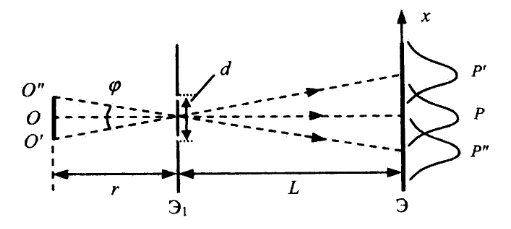
\includegraphics[scale = 0.6]{22_1}
	 \end{figure}
	 Пусть источник света имеет какие-то линейные размеры. Тогда каждая точка источника создает свою интерференционную картину, которые наслаиваются друг на друга. Как известно период полос $\dfrac{\lambda L}{d}$ а сдвиг за счет неточечности будет $\phi L$ итого получаем условие $b < \dfrac{\lambda}{\phi}$ это и называют радиусом когерентности. $ \rho = \dfrac{\lambda}{\phi}$

	
	\newpage
	
	\section{Пространственная когерентность. Степень пространственной когерентности. Звездный интерферометр Майкельсона и его современные модификации. } 
\subsection{Пространственная когерентность.}

\Def{Пространственная когерентность}  --  когерентность колебаний, которые совершаются в один и тот же момент времени в разных точках плоскости, перпендикулярной направлению распространения волны.
Вводится для объяснения интерференции нескольких источников.
Два источника называются пространственно когерентными, если их размеры и расположение позволяют наблюдать интерференцию.
\begin{theor}\label{2  некогерентных точечных источника.}

Условие для хорошей контрастности интерференционной картины($\alpha$ - правильная дробь):
\begin{equation}
\Delta = l[\cos{\beta_1}-\cos{\beta_2}]=(m+\alpha)\lambda, \alpha \in [0, 1/4]\label{23.1}
\end{equation}

Максимумы и минимумы накладываются:
\begin{equation}
\Delta = l[\cos{\beta_1}-\cos{\beta_2}]=m\lambda \label{23.2}
\end{equation}

Компенсируются:
\begin{equation}
\Delta = l[\cos{\beta_1}-\cos{\beta_2}]=(m+1/2)\lambda\label{23.3}
\end{equation}
\end{theor}
\begin{proofn}
Рассмотрим интерференцию от двух точечных источников A и B. P-точка интерференции. Из точки A исходят два луча: $AM_1P$ и $AM_2P$, которые друг с другом интерферируют в точке P. Аналогично для точки B есть 2 луча $BN_1P$ и $BN_2P$. 
\begin{figure}[H]
\center{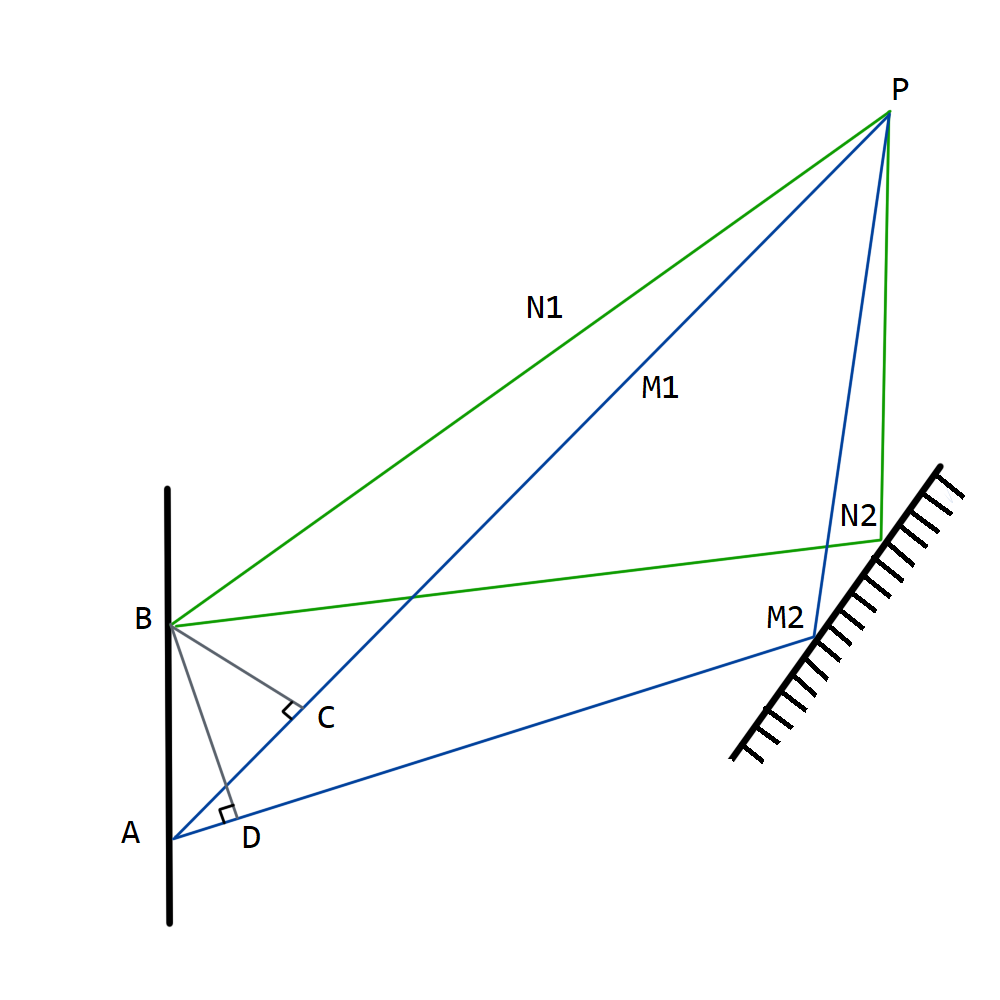
\includegraphics[scale=0.3]{8}}
\end{figure}
Если расстояние $AB=l$ мало, оптическая разность хода лучей от A и B:
$$\Delta_A=(AM_1P)-(BN_1P)=(AC)=\cos{BAC}=\cos{\beta_1}$$
$$\Delta_B=(AM_2P)-(BN_2P)=(AD)=\cos{BAD}=\cos{\beta_2}$$
 И результирующая разность хода:

$\Delta=|\Delta_A-\Delta_B|=l|\cos{\beta_1}-\cos{\beta_2}|$  --характеризует относительный сдвиг двух независимых интерференционных картин

$\Delta \sim 0$ или $\Delta \sim \lambda$, сдвиг нулевой$\qrq$максимумы и минимумы складываются.

$\Delta \sim \lambda$,  максимумы накладываются на минимумы$\qrq$ интерференционная картина пропадает.

Очевидно, при сдвиге на целое число длин волн картина не меняется.
Условие \ref{23.1} отражает промежуточное состояние, может показаться произвольным, но ним так будет удобно в будущем.
\end{proofn}
\begin{theor}\label{Протяженный источник длины l.}
Разобьем источник на пары некогерентных точек $(A_1 B_1), (A_2 B_2), ... $ находящихся на расстоянии l/2. Для каждой из них можно записать условие \ref{23.3}: 
\\$\frac{l}{2}||\cos{\beta_1}-\cos{\beta_2}|=\frac{\lambda}{2}$ или $\delta= l[\cos{\beta_1}-\cos{\beta_2}]=\lambda$ 

То есть каждая пара не дает интерференционных полос$\qrq$мы видим равномерный светлый фон.
Аналогично, если $\delta=(m+\alpha)\lambda$, где $\alpha$ правильная дробь, мы можем разбить источник на две части в пропорции $m:\alpha$. Меньшая часть будет создавать полосы на светлом фоне, создаваемом большей частью. Чем больше m, тем хуже видно интерференцию.

Условие хорошей контрастности:
$\delta= l[\cos{\beta_1}-\cos{\beta_2}]|\leq \lambda/2$
\\Если существует точка, из которой лучи исходят симметрично, т.е $\beta_2=\pi-\beta_1$, угол между этими лучами - угол интерференции $\Omega = \beta_2-\beta_1=\pi - 2\beta_1$.
$$|\cos{\beta_1}-\cos{\beta_2}|=2\cos{\beta_1}=\sin({\frac{\pi}{2}-\beta_1})=\sin{\frac{\Omega}{2}}$$ %РИСУНОК
В этом случае условие хорошей контрастности: 
$ l\frac{\sin{\Omega}}{2}\leq \lambda/4$ 
\end{theor}
\subsection{Степень пространственной когерентности.}
Для определения степени когерентности вообдят понятие 

\Def{Корреляционная функция} -- Зависящая от времени корреляция двух случайных функций $E(r_1, t_1)$ и $E(r_2, t_2)$ определяется как $B(r_1, t1, r_2, t_2)\langle E(r_1, t_1) E(r_2, t_2)\rangle$, где угловые скобки обозначают процедуру усреднения.  

\Def{Степень когерентности}
Для светового пучка введем величину $$\gamma(r_1,r_2, t=t_1-t_2)=\frac{B}{\sqrt{I_1I_2}}$$ -- комплексную степень когерентности. $\gamma\leq1$ 
При t=0 $|\gamma|$ -- степень пространственной когерентности, а при $r_1=r_2$ -- степень временной когерентности.
\subsection{Звездный интерферометр Майкельсона}
Если поставить на пути лучей источника экран с двумя отверстиями, расположенными на расстоянии D, появляется специфицеская картина. Если закрыть одно отверстие, то дифракция лучей на втором даст стандартную картину колец, однако если открыть оба отверстия, две системы колец совместятся. К эффекту обычного сложения минимумов и максимумов добавится интерференция двух щелей и кольца будут пересечены интерференционными полосами. Угловое расстояние между этими полосами определяется угловым расстоянием -- углом, на который отличаются направления на соседние интерференционные максимумы:$\upsilon=\lambda/D$.
Допустим, мы наблюдаем в такую систему двойную звезду с угловым расстоянием $\delta\phi=\upsilon/2$ между ее компонентами. Тогда минимумы интерференционных полос от одной звезды наложатся на минимумы другой. Изменяя расстояние D можно добиться картины, на которой интерференционные полосы пропадут совсем или их видимость станет наименьшей.  В таком случае угловое расстояние между компонентами звезды станет 
$$\delta\phi=\frac{\lambda}{2D}$$
Для одиночной звезды можно применить тот же метод: для упрощения вычислений можно проедполоэить, что звезда излучает как квадрат, плоскоссть которого параллельная фокальной плоскости объектива, а пара сторон параллельная прямой, соеддиняющей отверстия экрана. Тогда можно разбить этот квадрат на пары полосок(аналогично случаю с протяженным источником в этом же билете), каждая пара не даст интерференционных полос. Подобрав D так, что интерференционные полосы исчезнут,угловой размер стороны квадрата можно найти по формуле   $\delta\phi'=\frac{\lambda}{D}$
Если звезду представить как равномерно светящийся диск, угловой размер можно найти по формуле $\delta\phi'=1,22\frac{\lambda}{D}$
Проблема этого метода в том, что для хорошей интерференции нужен телескоп с большим диаметром объектива. Майкельсон соединил телескоп с интерферометром и решил эту проблему, добавив зеркала.
\begin{figure}[H]
\center{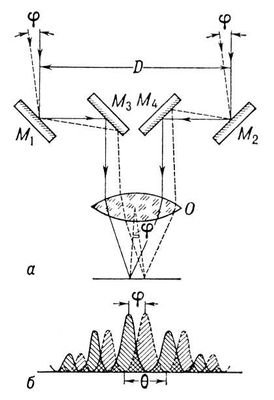
\includegraphics[scale=0.5]{9}}
\end{figure}
Изменяя расстояние между отверстиями и перемещая зеркала, можно добиться исчезновения интерференционной картины.
\subsubsection{Принцип работы звездного интерферометра Майкельсона}
По принципу Гюйгенса-Френеля заменим звезду на вторичный фронт(уберем звезду, поместим вторичные источники $S_1$ и $S_2$ в отверстия экрана.) Зеркала дадут 2 пары мнимых изображений. Если от звезды идет пучок параллельных лучей, то источники, а значит, и их изображения, будут в одной фазе. Получается, что зеркала позволяют "сблизить" вторичные источники, а интерференционная картина сохранится. 

Теперь расположим вторую звезду на расстоянии $\delta\phi$ от первой. Ее волновой фронт будет достигать отверстий не одновременно(нет симметрии) Разность хода между лучами, приходящими в отверстия, будет равна $D\delta\phi$. Интерференционные полосы минимизируются, если разность хода будет равна $D\delta\phi=\lambda/2$. Получилась формула, идентичная старой модели телескопа.

Проблема телескопа такой конструкции в том, что система зеркал  должна быть строго неподвижной и при этом раздвигаться на большое расстояние.
\subsubsection{Современные модификации.}
Я не имею ни малейшего понятия, что тут имеется в виду, но вот что накопалось в гугле:
\begin{figure}[H]
\center{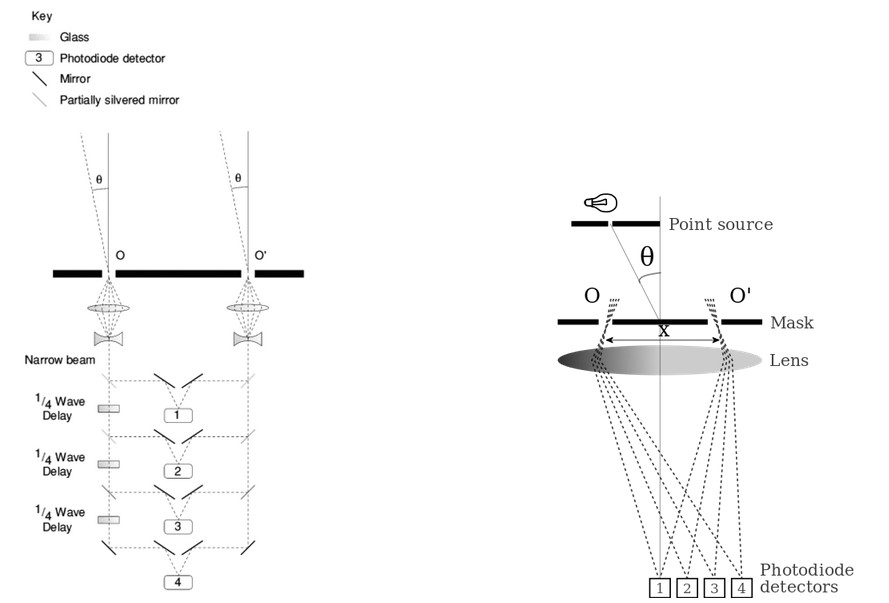
\includegraphics[width=\textwidth]{10}}
\caption{Слева: двухэлементный оптический интерферометр. Справа: Интерферометр с дополнительной диафрагмой.}
\end{figure}
Простой двухэлементный интерферометр устроен следующим образом: Свет от двух телескопов(на схеме изображены как линзы) с помощью системы пластинок и зеркал направляется в 4 независимых детектора. Пластинки обеспечивают фазовую задержку и позволяет измерить видность изображения.
 
В телескопе с диафрагмой используется несколько датчиков, во которые свет будет попадать, пройдя один и тот же оптический путь, что позволяет увеличить точность измерений.
	
	\newpage
	
	
\section{Полосы равной толщины и равного наклона. Интерференция света на тонких пленках. Кольца Ньютона.}

\subsection{Интерференция волн при отражении от пластины. Полосы равного наклона.}

Пусть луч падает на плоскопараллельную пластину толщиной  $h$ с показателем преломления $n$ под некоторым углом $\alpha$ к нормали. Этот луч может сразу отразиться от верхней поверхности (порождая луч 1), а может сначала попасть внутрь пластины, а затем, отразившись от нижней грани, выйти из пластины через верхнюю поверхность (порождая луч 2). В результате каждый луч расщепляется на два, которые могут интерферировать между собой.
\begin{figure}[h!]
    \centering
    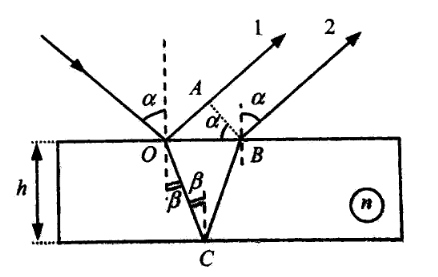
\includegraphics[scale=1]{plas.png}
    \caption{К расчету интерференции волн при отражении от пластины}
    \label{fig:my_label}
\end{figure} 

\bigskip

Найдем оптическую разность хода лучей 1 и 2. Проведем отрезок $AB$ перпендикулярно лучам 1 и 2. Тогда искомая длина набирается на трассах лучей до их пересечения с отрезком $AB$ и составляет

\begin{equation*}
    \delta_1 = L_2 - L_1 = n\cdot OCB - OA.
\end{equation*}

Длина трассы луча 2 в пластине составляет

\begin{equation*}
    OCB = \frac{2h}{\cos\beta},
\end{equation*}
где $beta$ - угол преломления, даваемый законом Снеллиуса:

\begin{equation*}
    \sin\alpha = n\sin\beta.
\end{equation*}


Для нахождения длины отрезка $OA$ найдем горизонтальный ход луча 2 в пластине:

 \begin{equation*}
     OB = 2h\tan\beta .
 \end{equation*}

Отсюда следует

 \begin{equation*}
     OA = OB\sin\alpha = 2h\tan\beta\sin\alpha .
 \end{equation*}
Таким образом, получаем
 \begin{equation*}
     \delta_1 = n\frac{2h}{\cos\beta} - 2h\tan\beta\sin\alpha = \frac{2hn}{\cos\beta}\left(1 - \frac{1}{n}\sin\beta\sin\alpha\right).
 \end{equation*}
С помощью закона Снеллиуса отсюда находим


 \begin{equation*}
    \delta_1 = 2hn\cos\beta = 2h\sqrt{n^2 - \sin^2\alpha}.
 \end{equation*}


Помимо полученной разности хода вклад в сдвиг фаз лучей может давать и отражение от поверхностей. Согласно формулам Френеля амплитудный коэффициент отражения при нормальном падении волны равен

\begin{equation*}
    r = \frac{E_{\text{отр}}}{E_{\text{пад}}} = \frac{1-n}{1+n}
\end{equation*}
 
 
 Следовательно, фаза волны меняется на $\pi $ при отражении от среды оптически более плотной и не меняется при отражении от среды оптически менее плотной. Такая же ситуация имеет место для $s-$поляризованной волны при падении под любыми углами. Для $p-$ поляризованной волны изменение фазы на $\pi$ имеет место для углов падения, не превышающих угла Брюстера. При больших же углах фаза волны не меняется.
 
 Таким образом, если угол падения не превышает угла Брюстера, то из найденной разности хода лучей $\delta$ следует вычесть поправку $\frac{\lambda}{2}$, обусловленную отражением луча 1 от оптически более плотной среды:
 
 \begin{equation*}
     \delta = \delta_1 - \frac{\lambda}{2}
 \end{equation*}
 
 Интерференционные максимумф интенсивности должны наблюдаться, если $\delta = m\lambda$, m = 0,1,2,..., или
 
\begin{equation*}
    2h\sqrt{n^2- \sin^2\alpha} = \left(m+\frac{1}{2}\right)\lambda .
\end{equation*}

Это равенство выделяет те углы падения лучей, при которых волны благодаря интерференции усиливаются. Если же выполняется условие $\delta = \left(m+\frac{1}{2}\right)\lambda$, или

\begin{equation*}
    2h\sqrt{n^2- \sin^2\alpha} = m\lambda ,
\end{equation*}

то происходит интерференционное гашение волн.

\medskip

Для наблюдения интерференционных полос на пути отраженных лучей следует поставить собирающую линзу.
Известно, что линза собирает параллельный пучок лучей в точку в фокальноф плоскости. Эта точка (в случае тонкой линзы) находится на пересечении фокальной плоскости с лучом, параллельным пучку и проходящим через оптический центр линзы. В зависимости от угла падения на пластину отраженные лучи будут собираться в разных точках фокальной плоскости. Пусть падающий на пластинку свет имеет разные направления (рассеяный свет). Тогда для лучей с направлениями, отвечающими интерференционному усилению, будут наблюдаться светлые полосы. Лучи же, для которых имеет место интерференционное подавление, будут на экране формировать темные полосы.


\begin{figure}[h!]
    \centering
    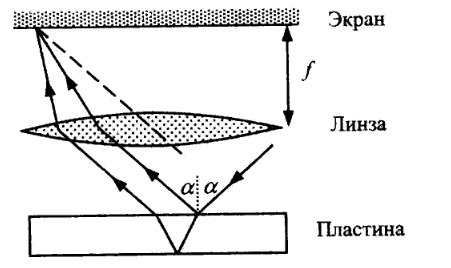
\includegraphics[scale=1]{plas2.png}
    \caption{Схема наблюдения интерференционных полос равного наклона при отражении света от пластины}
    \label{fig:my_label}
\end{figure} 
Поскольку в данном эксперименте каждая из полос формируется только группой лучей с одним и тем же углом падения (наклона), то такии линии на экране называются \textit{полосами равного наклона}.
\subsection{Полосы равного наклона}
\subsection{Кольца Ньютона}

Схема опыта: свет падает на линзу с большим радиусом кривизны, лежащую на плоскопараллельной стеклянной пластинке. Регистрируется излучение, отраженное системой или прошедшее через нее. Оказалось, что при нормальном падении света на сферической поверхности локализована серия колец - интерференционных полос.


\begin{figure}[h!]
    \centering
    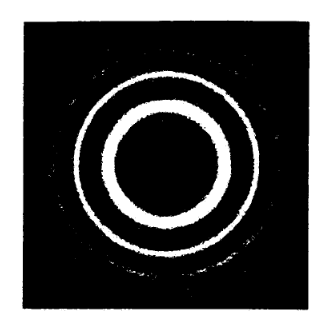
\includegraphics[scale=1]{anal_rings2.png}
    \caption{Кольца Ньютона в отраженном свете}
    \label{fig:my_label}
\end{figure} 

Зазор между линзой и пластинкой играет роль, аналогичную клину. Интерференция возникает между лучами, отраженными от пластинки и от кривой поверхности линзы. Разность хода отраженных лучей зависит от толщины зазора $d$ в месте падения луча 1 и составляет $2d$. Найдем ее.

\bigskip



\begin{figure}[h!]
    \centering
    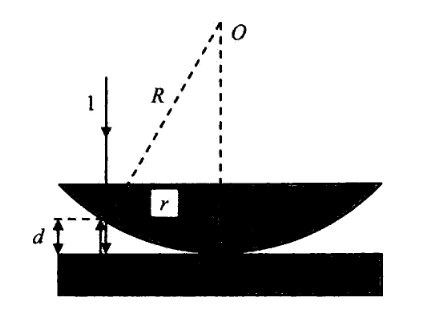
\includegraphics[scale=1]{anal_rings1.png}
    \caption{Схема оптической системы, в которой наблюдаются кольца Ньютона}
    \label{fig:my_label}
\end{figure} 
Пусть радиус кривизны линзы равен $R$. Тогда из теоремы Пифагора находим

\begin{equation*}
    R^2 = r^2 + (R-d)^2 \Rightarrow 2Rd = r^2/
\end{equation*}

Здесь, считая зазор тонким в области наблюдения, мы пренебрегли малой величиной $d^2$ по сравнению с удержанными слагаемыми. При отражении луча от оптически более плотной среды волны приобретает дополнительный сдвиг фазы,  соответствующий дополнительной разности хода $\frac{\lambda}{2}$. Поэтому находим оптическую разность хода лучей, отраженных от линзы и пластинки:

\begin{equation*}
    \Delta = 2d + \frac{\lambda}{2} = \frac{r^2}{R} + \frac{\lambda}{2}.
\end{equation*}

Темные кольца отвечают интерференционным минимумам интенсивности, наблюдающимся при условии $\Delta = (m+1/2)\lambda$, откуда находим радиусы темных колец:

\begin{equation*}
    r_m = \sqrt{m\lambda R}, \hspace{10px} m = 0,1,2,...
\end{equation*}

Из условия $\Delta = m\lambda$ получаем радиусы светлых колец:

\begin{equation*}
    r_m = \sqrt{(m-1/2)\lambda R}, \hspace{10px} m = 1,2,...
\end{equation*}

Таким образом, в отраженном свете центр колец темный. Если бы мы рассматривали прошедший свет, то добавка $\frac{\lambda}{2}$ к разности хода не возникала вследствии того, что отраждение луча от оптически более плотной среды двукратное. Соответственно темные и светлые кольца меняются местами, причем центр колец оказывается светлым.

В заключение можно отметить следующее:

\begin{enumerate}
    \item Наблюдающиеся кольца являются полосами \textit{равной толщины}, поскольку их положение зависит от толщины зазора: волны, проходящие участки зазора, имеющие одну и ту же толщину, но в разных точках вокруг оси системы, образуют одно кольцо.
    \item Радиусы колец зависят от длины волны. В случае немонохроматического света каждое кольцо будет иметь различную окраску в разных его точках: в точках, более удаленных от центра, окраска смещается в красную область спектра.
    \item В расчетах выше показатель преломления между линзой и пластинкой был равен единице. Если это не так, будет меняться разность хода отраженных лучей, приводя к изменению радиусов колец Ньютона.
    \item Кольца Ньютона используются для измерения радиусов кривизны поверхностей, длин волн света и показателей преломления.
\end{enumerate}


	
	\newpage
	
	\section{Двухлучевые интерферометры. Интерферометры Рэлея, Маха-Цендера, Майкельсона. Применение интерферометров в научных исследованиях и технике: измерение малых смещений, изучение состояния поверхности, рефрактометрия (изменение показателя преломления). }
	\subsection{Двухлучевые интерферометры.}
	\begin{definition}
		Интерферометром называется измерительный прибор основным действие которого основано на явлении интерференции.  Принцип действия интерферометра заключается в следующем: пучок электромагнитного излучения с помощью того или иного устройства пространственно разделяется на два или большее количество когерентных пучков. Каждый из пучков проходит различные оптические пути и направляется на экран, создавая интерференционную картину, по которой можно установить разность фаз интерферирующих пучков в данной точке картины.
	\end{definition}
	\begin{definition}
		Двулучевыми называются интерферометры использующие в своей работе два когерентных пучка, идущих разными оптическими путями.
	\end{definition}
\subsection{Интерферометр Рэлея}
\begin{figure}[H]
	\centering
	\begin{tikzpicture}[>=latex']
	\draw[red,thick,->] (-2.9,0) -- (-2.5,0);
	\draw[red,thick,->] (-2.94,0.04) -- (-2.55,0.2);
	\draw[red,thick,->] (-2.94,-0.04) -- (-2.55,-0.2);
	\filldraw[fill=red!44!white,draw=black] (-3,0) circle (0.1) node[left] {\scriptsize{Источник}}; 
	\draw[black!77!red,thick] (-2.45,1) -- (-2.45,-1);
	\draw[white,thick] (-2.45,0.05) -- (-2.45,-0.05);
	\filldraw[fill=blue!11!white,draw=black] (-2,-0.5) arc (210:150:1) -- (-1.95,0.5) arc (30:-30:1) -- cycle;
	\draw[black!77!red,thick] (-1.5,1.2) -- (-1.5,-1.2);
	\draw[white,thick] (-1.5,0.35) -- (-1.5,0.45);
	\draw[white,thick] (-1.5,-0.35) -- (-1.5,-0.45);
	\filldraw[fill=green!11!white,draw=black, thick] (-1.2,0.2) -- (-1.2,0.6) -- (0.5,0.6) -- (0.5,0.2) -- cycle node[above, pos=0.5]{\scriptsize $n_{1}$};
	\filldraw[fill=green!33!white,draw=black, thick] (-1.2,-0.2) -- (-1.2,-0.6) -- (0.5,-0.6) -- (0.5,-0.2) -- cycle node[below, pos=0.5]{\scriptsize $n_{2}$};
	\filldraw[fill=blue!11!white,draw=black] (0.7,-0.15) -- (0.7,-0.65) -- (0.85,-0.65) -- (0.85,-0.15) -- cycle;
	\filldraw[fill=blue!11!white,draw=black] (0.7,0.15) -- (0.7,0.65) -- (0.85,0.65) -- (0.85,0.15) -- cycle;
	\filldraw[fill=blue!11!white,draw=black] (1.55,-0.5) arc (210:150:1) -- (1.6,0.5) arc (30:-30:1) -- cycle;
	\filldraw[fill=gray!44!white,draw=black] (2.2,0.3) -- (2.2,-0.3) -- (3.2,-0.3) -- (3.2,0.3) -- cycle;
	\node at (3.9,0) {\scriptsize{Детектор}};
	\draw[red] (-2.45,0) -- (-1.925,0.4);
	\draw[red] (-2.45,0) -- (-1.925,-0.4);
	\draw[red,->] (-2.45,0) -- (-2.2,0.2);
	\draw[red,->] (-2.45,0) -- (-2.2,-0.2);
	\draw[red] (-1.925,0.4) -- (-0.55,0.4);
	\draw[red] (-1.925,-0.4) -- (-0.55,-0.4);
	\draw[red,->] (-1.95,0.4) -- (-0.9,0.4);
	\draw[red,->] (-1.95,-0.4) -- (-0.9,-0.4);
	\draw[red] (-0.2,0.4) -- (1.625,0.4);
	\draw[red] (-0.2,-0.4) -- (1.625,-0.4);
	\draw[red,->] (-0.2,0.4) -- (1.3,0.4);
	\draw[red,->] (-0.2,-0.4) -- (1.3,-0.4);
	\draw[red] (1.625,0.4) -- (2.2,0);
	\draw[red] (1.625,-0.4) -- (2.2,0);
	\draw[red,->] (1.625,0.4) -- (1.9125,0.2);
	\draw[red,->] (1.625,-0.4) -- (1.9125,-0.2);
	\end{tikzpicture}
	\caption{Интерферометр Рэлея}
	\label{rel}
\end{figure}
Интерферометр Рэлея представлен на рис.~\ref{rel}.
Свет от источника пропускается через линзу, создающую параллельный пучок, и апертуры, вырезающие из него два луча (плечи интерферометра). Каждый из лучей проходит сквозь собственную кювету с газом со своим показателем преломления ($n_{1}$ и $n_{2}$). На выходе схемы расположена линза, сводящая оба пучка вместе для получения интерференционных полос в её фокусе.

Для измерений в одно из плеч вносится компенсатор — например, стеклянная пластинка, с помощью поворота которой можно изменять оптическую длину пути луча в плече. Если показатель преломления в одном из плеч равен $n_{1}$, то второй неизвестный показатель преломления равен
\begin{equation*}
n_{2} = n_{1} + \frac{\lambda_{0}}{\ell}\Delta m
\end{equation*}
где $\ell$ -- длина кюветы с газом, $\lambda _{0}$ -- длина волны источника света, $\Delta m$ -- порядок интерференции (количество пересекающихся в заданной точке интерференционных полос). При типичных параметрах установки — длине кювет в один метр, длине волны в 550 нм и порядке интерференции 1/40, — можно измерить разницу показателей преломления, равную $10^{-8}$. Чувствительность интерферометра определяется длиной кюветы. Её максимальная длина, как правило, определяется техническими возможностями контроля за температурой, так как тепловые флуктуации будут искажать показатели преломления газов.
	\subsection{Интерферометр Маха-Цендера}
	\begin{figure}[H]
		\centering
		\begin{tikzpicture}[>=latex']
		\filldraw[fill=gray!44!white,draw=black] (-3,-2.1) -- (-2.5,-2.1) -- (-2.5,-1.9) -- (-3,-1.9) -- cycle node[below] {\scriptsize{Источник}}; 
		\draw[blue!22!white,very thick] (-1.7,-2.2) -- (-1.3,-1.8);
		\draw[blue!22!white,very thick] (1.4,-1.8) -- (1,-2.2);
		\draw[black!66!white,very thick] (1.43,-1.83) -- (1.03,-2.23);
		\draw[blue!22!white,very thick] (1.0,0.5) -- (1.4,0.9);
		\draw[blue!22!white,very thick] (-1.7,0.5) -- (-1.3,0.9);
		\draw[black!66!white,very thick] (-1.73,0.53) -- (-1.33,0.93);
		\filldraw[fill=gray!44!white,draw=black] (1.0,1.6) -- (1.4,1.6) -- (1.4,1.3) -- (1.0,1.3) -- cycle node[above] {\scriptsize{Детектор}};
		\filldraw[fill=gray!44!white,draw=black] (2.0,-2.2) -- (2.3,-2.2) -- (2.3,-1.8) -- (2.0,-1.8) -- cycle node[below] {\scriptsize{Детектор}};
		\draw[red] (-2.5,-2) -- (2.0,-2);
		\draw[red,->] (-2.5,-2) -- (-2.0,-2);
		\draw[red,->] (-2.5,-2) -- (0.0,-2);
		\draw[red,->] (-2.5,-2) -- (1.75,-2);
		\draw[red] (1.2,-2) -- (1.2,1.3);
		\draw[red,->] (1.2,-2) -- (1.2,0);
		\draw[red] (-1.5,-2) -- (-1.5,0.7);
		\draw[red,->] (-1.5,-2) -- (-1.5,0.0);
		\draw[red] (-1.5,0.7) -- (1.2,0.7);
		\draw[red,->] (-1.5,0.7) -- (0,0.7);
		\draw[red,->] (1.2,0.7) -- (1.2,1.1);
		\end{tikzpicture}
		\caption{Схема интерферометра Маха-Цендера}
		\label{mach}
	\end{figure}
	Интерферометр Маха-Цендера устроен следующим образом (Рис.~(\ref{mach})).
	На входе интерферометра находится полупрозрачное зеркало, расщепляющее световой поток на два луча. Они сводятся вместе после отражения от двух непрозрачных зеркал в четвёртом зеркале. Зеркала интерферометра образуют параллелограмм. Для проведения исследований в одно из плеч интерферометра помещают ёмкость с исследуемым газом и компенсаторы.
	\subsection{Интерферометр Майкельсона}
	\begin{figure}[H]
		\centering
		\begin{tikzpicture}[>=latex']
		\filldraw[fill=gray!44!white,draw=black] (-3,-0.1) -- (-2.5,-0.1) -- (-2.5,0.1) -- (-3,0.1) -- cycle node[below] {\scriptsize{Источник}};
		\filldraw[fill=gray!44!white,draw=black] (-0.1,-2.5) -- (0.1,-2.5) -- (0.1,-3) -- (-0.1,-3) -- cycle node[left] {\scriptsize{Детектор}}; 
		\draw[blue!22!white,very thick] (-0.3,-0.3) -- (0.4,0.4);
		\draw[blue!22!white,very thick] (2.95,-0.3) -- (3.05,0.3);
		\draw[black!66!white,very thick] (2.99,-0.308) -- (3.09,0.292) node[right] {\scriptsize{Зеркало}};
		\draw[red] (3,0) -- (0.2,0.2);
		\draw[blue!22!white,very thick] (-0.3,2.5) -- (0.3,2.5);
		\draw[black!66!white,very thick] (-0.3,2.54) -- (0.3,2.54) node[above] {\scriptsize{Зеркало}};
		\draw[red] (0.2,0.2) -- (0,-2.5);
		\draw[red,->] (-2.5,0) -- (-1.5,0);
		\draw[red] (3,0) -- (0.2,0.2);
		\draw[red,->] (0.2,0.2) -- (0.1,-1.15);
		\draw[red,->] (0,0) -- (1.3,0);
		\draw[red,->] (3,0) -- (1.6,0.1);
		\draw[red] (0,-2.5) -- (0,2.5);
		\draw[red,->] (0,0) -- (0,1);
		\draw[red,->] (0,2.5) -- (0,1.75);
		\draw[red] (-2.5,0) -- (3,0);
		\draw[red,->] (0,0) -- (0,-1.5);
		\node at (1.3,0.8) {\scriptsize{Cветоделительное}};
		\node at (1.1,0.5) {\scriptsize{зеркало}};
		\end{tikzpicture}
		\caption{Схема интерферометра Майкельсона}
		\label{michelson}
	\end{figure}
Интерферометр Майкельсона (рис.~\ref{michelson}) -- двулучевой интерферометр. Конструктивно состоит из светоделительного зеркала, разделяющего входящий луч (выходящий из источника когерентного излучения) на два, которые в свою очередь, отражаются зеркалом обратно. На полупрозрачном зеркале разделённые лучи вновь направляются в одну сторону, чтобы, смешавшись на экране, образовать интерференционную картину. Анализируя её и изменяя длину одного плеча на известную величину, можно по изменению вида интерференционных полос измерить длину волны, либо, наоборот, если длина волны известна, можно определить неизвестное изменение длин плеч. Радиус когерентности изучаемого источника света или другого излучения определяет максимальную разность между плечами интерферометра.
\subsection{Применение интерферометров в научных исследованиях и технике: измерение малых смещений, изучение состояния поверхности, рефрактометрия (изменение показателя преломления).}
В силу того, что интерферометры очень чувствителны к изменению оптического хода лучей в них, при помощи интерферометров часто измеряются малые расстояния.
Рефрактометрия -- метод исследования веществ, основанный на определении показателя (коэффициента) преломления (рефракции) и некоторых его функций. Как видно выше при помощи интерферометров можно измерять показатели преломления различных веществ за счёт изменения разности хода различных световых пучков внутри интерферометра.
	
	\newpage
	
	\section{Интерферометр Майкельсона. Фурье-спектрометр. Применение интерферометров в научных исследованиях}

\subsection{Интерферометр Майкельсона}

Схема интерферометра представлена на рисунке. 

\begin{figure}[H]
	\centering
	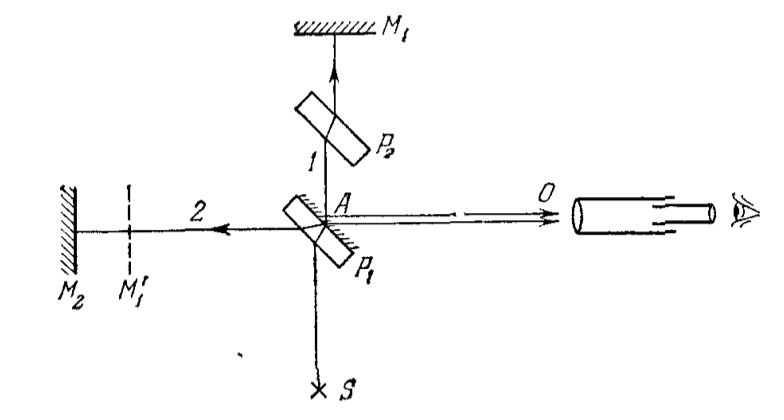
\includegraphics[width=\linewidth]{26_1}
	\caption{Интерферометр Майкельсона}
\end{figure}

Приведем краткое описание:

Свет от некоторого протяженного источника $S$ попадает на плоскопараллельную полупрозрачную пластинку $P_1$. Она разделает попавший на нее пучок на два, первый и второй соответственно. Первый пучок, после прохождения пластинки, отражается обратно \textbf{статичным} зеркалом $M_1$, после чего частично отражается от пластинки $P_1$ в указанном направлении. Второй же пучок, отразившись от границы пластинки $P_1$, направляется к зеркалу $M_2$, после чего проходит через пластинку $P_1$ и идет совместно с пучком 1. Отметим, что второй пучок проходит пластину $P_1$ трижды. Чтобы исключить получающуюся из-за этого разность фаз, на пути первого пучка ставят пластинку $P_2$, идентичную $P_1$.

Пусть $M_1'$ --- изображение зеркала $M_1$ в отражающей плоскости пластинки $P_1$. Тогда происходящая интерференция равносильна интерференции в воздушном слое между $M_1'$ и $M_2$. Разность хода между лучами составляет $\Delta = 2 d\cos \phi$, где $d$ --- толщина слоя, $\phi$ --- угол падения. Если слой плоскопараллелен, то мы получим интерференционные кольца с центром в точке схождения лучей, нормально отраженных от поверхностей $M_1'$ и $M_2$. Этому направлению соответствует максимальная разность хода $\Delta = 2 d$, значит максимальный порядок интерференции будет в центре. При увеличении $d$ полосы будут перемещаться от центра; при увеличении зазора на $d = \lambda/2$, произойдет смещение картины на одну полосу (т.е. на место светлой полосы снова придет светлая), т.к. $\Delta = \lambda$. Если же мы измени угол падения, то разность хода изменится на $\Delta = 2 d \sin\phi \Delta\phi$. Полосы получаются чем шире, чем меньше $d$, т.е. при $d = 0$ мы получим равномерное освещение.

Интерферометр использовался, например, при проведении  \href{https://elementy.ru/trefil/21167/Opyt_MaykelsonaMorli}{опыта Майкельсона -- Морли}, в ходе которого было установлено отсутствие движения Земли относительно эфира.

\subsection{Фурье-спектрометр}

Схема спектрометра представлена на рисунке. 

\begin{figure}[H]
	\centering
	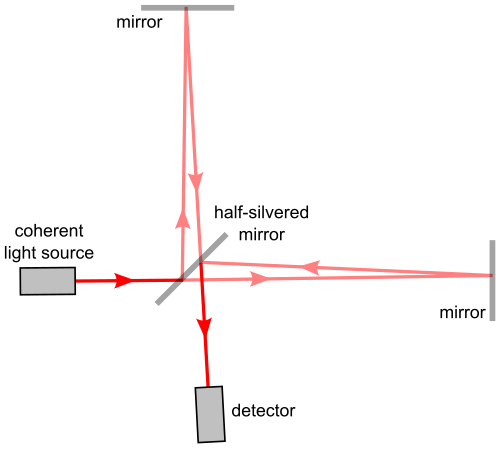
\includegraphics[width=\linewidth]{26_2}
	\caption{Фурье=спектрометр}
\end{figure}

Приведем краткое описание:

Основой спектрометра является интерферометр Майкельсона (только он тут почему-то без второй пластины, ха-ха). Предположим, что у нас есть некоторый когерентный источник излучения с длиной волны $\lambda$. Когда разность хода лучей в спектрометре оказывается равной $\lambda/2$, интенсивность регистрируемого света оказывается близкой к нулю. При перемещении правого зеркала интерферометра Майкельсона разность хода лучей изменяется, изменяется и интенсивность света, регистрируемая приёмником. Очевидно, что интенсивность света максимальная, когда разность хода лучей будет кратна длине волны $\lambda$.

При перемещении зеркала с постоянной скоростью на выходе приёмника будет наблюдаться электрический сигнал синусоидальной формы. Притом период синусоиды зависит от длины волны источника, а амплитуда от интенсивности источника.

Теперь представим, что на входе некогерентный источник. Каждая длина волны в спектре источника света будет давать свою синусоиду на выходе приёмника. Таким образом, на выходе приёмника мы получаем сложный сигнал. При выполнении над полученным сигналом обратного преобразования Фурье получаем спектр входного электрического сигнала, который также является спектром излучения источника (то есть интенсивность излучения источника на различных длинах волн).

За счет этого можно проводить спектральные анализы для выявления состава газов или жидкостей. Каждый газ или жидкость имеет свой спектр поглощения проходящего через него излучения. Таким образом спектр на входе интерферометра будет иметь «провалы» на определённых длинах волн. После обратного преобразования Фурье получаем спектр поглощения, по которому достаточно просто определить присутствующие в анализируемом воздухе газы и их концентрацию.

\subsection{Применение интерферометров в научных исследованиях}

Фактически, интерферометр позволяет с большой точностью измерять расстояния, поэтому его можно применять для создания деталей, изготовление которых требует высокой точности (сдвиг в интерференционной картине будет виден даже при небольшом отклонении).

Интерференционные методы позволяют с высокой точностью выявлять очень малые изменения показателя преломления среды, которые влияют на изменение оптической длины пути, а значит, влекут за собой изменение интерференционной картины.

Можно также измерять и углы.
	
	\newpage
	
	
	\section{Многолучевая интерференция. Интерферометр Фабри-Перо. Формула Эйри.
		Пластинка Люммера-Герке. Интерференционные фильтры и зеркала. Просветление
		оптики.}
	\begin{figure}[h]
		\centering
		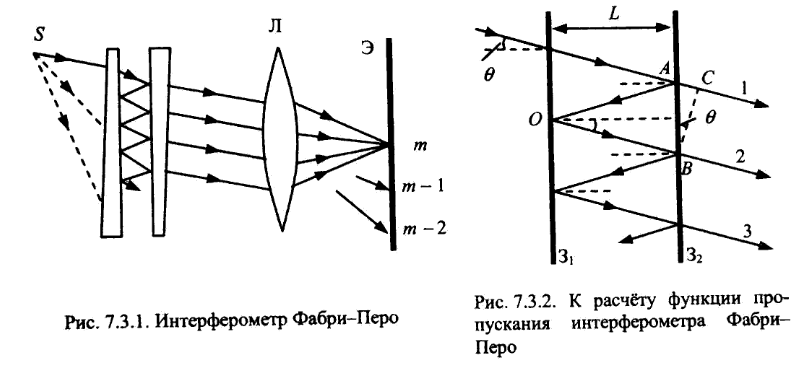
\includegraphics[scale = 0.7]{27_1}
	\end{figure}
	Интерферометр Фабри-Перо это два почти идеальных зеркала, которые отражают $\sim 99\%$ а оставшееся пропускают. Луч, попадая в нее испытывает многократные отражения. Обычно после интерферометра ставят линзу, что бы собрать параллельный пучек в точку.  Итак, пусть луч падает под углом $\theta$ на интерферометр. Надо думать, что он маленький, иначе не множественных отражений просто не будет. За один проход луч неберает фазу $\Delta = AOC - AB = \dfrac{2L}{\cos \theta} - 2L \tan \theta \sin \theta = 2L \cos \theta$ получается условие на максимумы будет иметь вид $2L \cos \theta = \lambda m$ \
	Пусть мы отражаемся много раз. Пусть на интерферометр падает луч с амплитудой $A$ и фазой ноль, тогда тот луч, который прошел ни разу не отразившись будет иметь $Ad^2$ тот который 2 раза отразился перед выходом $Ad^2 r^2 e^{i\delta}$  и так далее. Если угол тета мал, то отражений будет очень много, а $r^2 <1$ то просуммировав ряд получим:
	 \begin{align*}
	 A_{конечная} = Ad^2 \dfrac{1}{1 - r^2 e^{i\delta}}\\
	 \delta = 2L k\cos \theta\\
	 D = \dfrac{(1 - r^2)^2}{1 - 2r^2 \cos \delta + r^4}
	 \end{align*}
	 D это энергетический коэффициент пропускания. Так же это называется формулой Эйри, если судить по презентациям лектора.\\
	 \begin{figure}[t!]
	 	\centering
	 	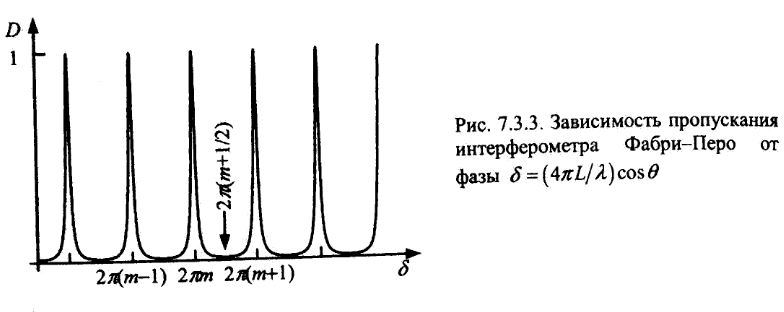
\includegraphics[scale = 0.5]{27_2}
	 \end{figure}
	 	Посмотрим на пластинку Люммера-Герке.
		\begin{figure}[h]
			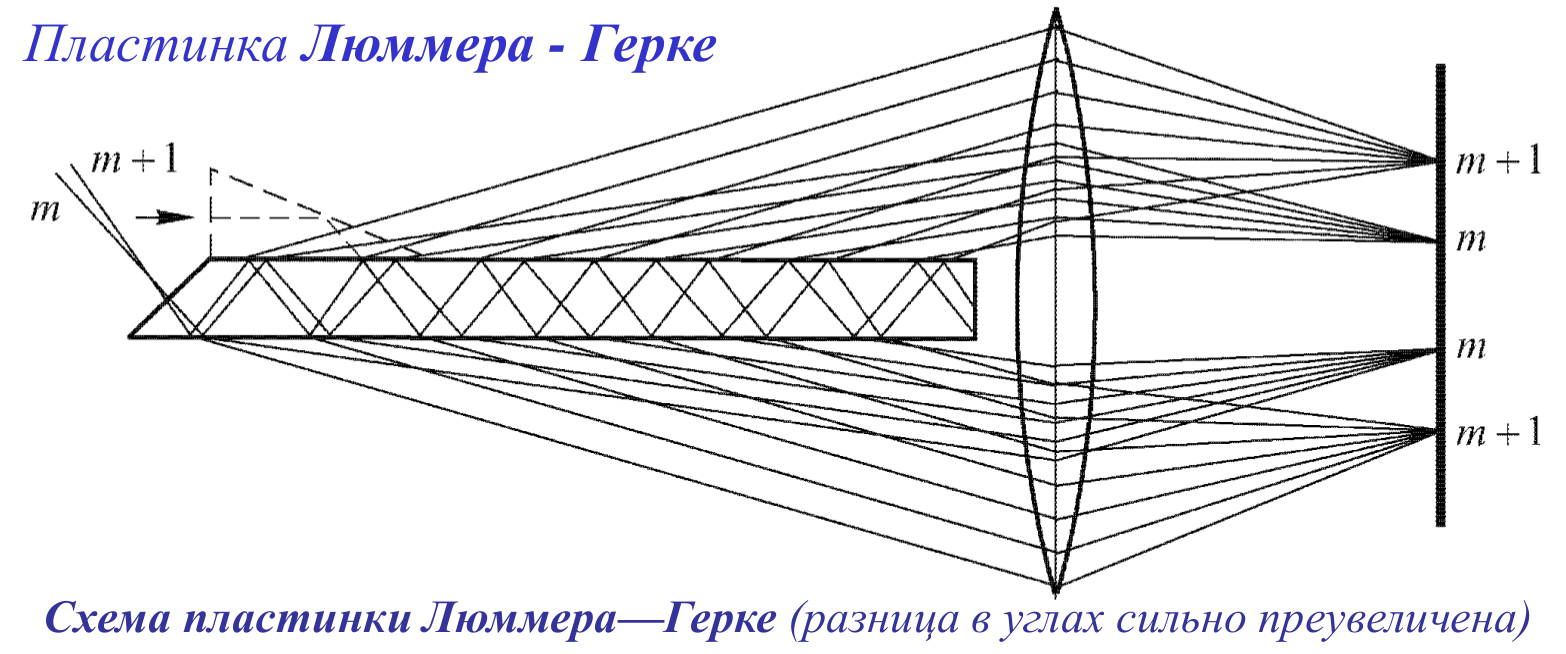
\includegraphics[scale = 0.3]{27_3}
		\end{figure}
		Что-то очень похожее на Фабри-Перо. Очевидно, что максимумы достигаются при условии $2d n \cos \theta = \lambda m$ где d толщина, а n- оптическая плотность \newpage
		\textbf{Просветление оптики}
		Допустим мы недовольны коэффициентом отражения стекла. Тогда мы можем нанести тонкий слой чего-нибудь на поверхность, главное чтобы это что-нибудь имело n меньше, чем у нашего стекла. При условии $\delta = \dfrac{2\pi}{\lambda} 2nh = (2m + 1)$ отраженная от первого края волна и отраженная от второго погасят друг друга и коэффициент прохождения увеличится.
		\begin{figure}[H]
			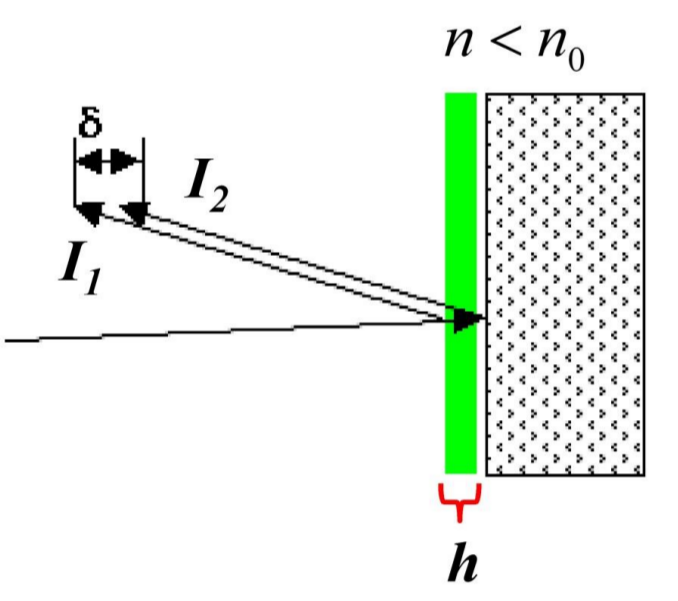
\includegraphics[scale = 0.3]{27_4}
		\end{figure}
	
	\newpage
	
	\section{Явление дифракции. Принципы Гюйгенса и Гюйгенса-Френеля. Понятие о теории дифракции Кирхгофа. Дифракция Френеля и дифракция Фраунгофера (ближняя и дальняя зоны дифракции). Волновой параметр.}

\Def{Дифракция света} -- уклонение от прямолинейного распространения, которое не является следствием отражения, преломления или изгибания света в среде. 

\Def{Принцип Гюйгенса}Каждая точка волнового фронта является источником сферических волн.

\Def{Принцип Гюйгенса-Френеля}Каждая точка поверхности, окружающей источники света, является источником вторичнных волн, распространяющихся во всех направлениях. Они когерентны, так как возбуждаются одними и теми же первичными источниками, результат их интерференции совпадает с исходным световым полем. 

\subsection{ Понятие о теории дифракции Кирхгофа.}
Основная идея Гюйгенса-Френеля в теории интерференции и дифракции волн света заключается в том, что световое возмущение в некоторой точке появляется как следствие наложения (суперпозиции) вторичных волн, которые испускаются поверхностью, расположенной между рассматриваемой точкой и источником света. Кирхгоф создал математическую форму записи принципа Гюйгенса-Френеля. Он показал, что вышеназванный принцип можно считать некоторой формой интегральной теоремы.
Интегральная теорема Кирхгофа дает возможность выразить амплитуду светового поля в точке наблюдения через интеграл по любой поверхности, которая охватывает точку наблюдения.

В теореме Кирхгофа решение однородного волнового уравнения в произвольной точке поля представлено через величину искомого параметра, его первую производную во всех точках произвольной замкнутой поверхности, которая окружает рассматриваемую точку.

Пусть волна будет монохроматической и скалярной:

\begin{equation*}
	U(r, t)=U_0(r, t)e^{(-i\omega t)}
\end{equation*}

$U_0$-комплексная амплитуда светового поля. В вакууме часть этой волны, зависящая от координат, удовлетворяет волновому уравнению Гельмгольца:

\begin{equation*}
	(\grad^2+\kappa^2)U_0=0
\end{equation*}

$\kappa=\frac{\omega}{c}$, так как само поле света удовлетворяет волновому уравнению.

Пусть V – объем, ограниченный произвольной замкнутой поверхностью S, точка А некоторая точка внутри рассматриваемого объема. Тогда одной из форм интегральной теоремы Кирхгофа – Гельмгольца:

\begin{equation*}
	U_0=\frac{1}{4\pi}\oint[{U_0\frac{\partial }{\partial n}(\frac{e^{i\kappa s}}{s})-\frac{e^{i\kappa s}}{s}\frac{\partial U_0}{\partial n}}]dS
\end{equation*}

где $\dfrac{\partial}{\partial n}$ – означает дифференцирование вдоль внутренней нормали к поверхности S. s – расстояние от точки А до точки с координатами (x,y,z).

\subsection{Дифракция Френеля. Ближняя зона дифракции}

Явления дифракции классифицируют в зависимости от расстояний источника и точки наблюдения (экрана) до препятствий, которые находятся на пути световой волны. Область дифракции, которая расположена недалеко от объекта, на котором происходит дифракция, называется ближней зоной дифракции или областью дифракции Френеля. Эта зона доходит до расстояний, с которых можно рассматривать дифракцию как фраунгоферову. В дифракционных задачах, использующих подходы Френеля нельзя пренебрегать кривизной поверхности волны, которая падает на препятствие (отверстие) и волны после дифракции. При дифракции Френеля на экране получают «дифракционное изображение» препятствия. Аналитический расчет дифракционных задач Френеля составляет существенные трудности.

\Def{Гипотеза Френеля} Для непрозрачного плоского экрана с отверстиями в качестве вспомогательной плоскости выберем неосвещенную сторону. Принцип Гюйгенса-Френеля позволяет свести задачу к определению поля на этой вспомогательной плоскости. На участках, перекрытых экраном, волновое поле 0, а на отверстиях оно определяется законами геометрической оптики. 

Недостатки теории:

\begin{enumerate} 
  \item Непонятно, как выбирать вспомогательную плоскость для неплоских экранов.
  
  \item Разрыв волнового поля на границах нарушает уравнения Максвелла.
  
  \item Если найти волновое поле во всем пространстве по принципу Гюйгенса-Френеля, оно не совпадет с исходным. Например, оно точно не обратится в нуль на задней стороне экрана.
  
  \item Гипотеза противоречит поперечности волн.
\end{enumerate}
В простейших случаях для того, чтобы установить вид картины дифракции используют метод кольцевых зон Френеля, спираль Корню. 

Особенности:

\begin{enumerate}
	\item Для оси пучка света считается, что интенсивность постоянна и равна интенсивности исходящей от источника интенсивности.\\ 2.Структура пучка света остается постоянной и задается формой отверстия. В пределах отверстия может располагаться множество зон Френеля. 
	
	\item Метод Френеля решения дифракционных задач может использоваться, когда размеры отверстий/препятствий $d\gg\lambda$, а значит, заметная интенсивность заметная при малых углах. Также, по гипотезе Френеля дифракционная картина не зависит от материала экрана.
\end{enumerate}

\subsection{Дифракция Фраунгофера. Дальняя зона дифракции}

Если расстояние между источником и экраном велико, дифракция называется дифракцией в параллельных лучах.

Область дифракции Фраунгофера простирается от бесконечности до некоторого минимального расстояния. На практике реализация дифракции Фраунгофера выполняется, если точечный источник световых волн размещают в фокусе собирающей линзы. Получившийся при этом параллельный пучок света совершает дифракцию на препятствии. Дифракционную картину наблюдают в фокальной плоскости линзы, которая размещается на пути света совершившего дифракцию или используют зрительную трубу, которую устанавливают на бесконечность. Картина дифракции является дифракционным изображением источника света. 

Особенностями дальней зоны дифракции являются: 

\begin{enumerate}
	\item Интенсивность исходной световой волны много больше, чем интенсивность света на оси пучка. 
	
	\item Интенсивность света на оси пучка уменьшается в зависимости от расстояния до источника (она обратно пропорциональна квадрату расстояния).
	
	\item Световой пучок, по мере распространения от источника, расширяется.
	
	\item В границах отверстия размещается только одна малая центральная часть зоны Френеля номер один.
\end{enumerate}	

\subsection{Волновой параметр}

\Def{Волновой параметр(число Френеля)} Определяет вид дифракции. Определяется формулой $p=\dfrac{\sqrt{\lambda z}}{b}$, где $\lambda$ - длина волны, $b$ --- размер отверстия, $z$ --- расстояние до плоскости (или до точки наблюдения):

\begin{itemize}
	\item $p<<1$ -- область геометрической оптики
	
	\item $p \sim 1$ -- область дифракции Френеля 
	
	\item $p>>1$ -- область дифракции Фраунгофера 
\end{itemize}
	
	\newpage
	
	\section{Дифракция Френеля. Простейшие дифракционные задачи. Дифракция на круглом отверстии и круглом экране, спираль Френеля. Пятно Пуассона. Распределение освещенности в дифракционной картине в поперечном направлении и вдоль оси отверстия.}

\textbf{Дифракция Френеля} (\textit{дифракция ближнего поля}) --- случай дифракции при \textit{волновом параметре} $p \approx 1$, где $p = \frac{\sqrt{L \lambda}}{d}$ ($L$ --- расстояние от препятствия, $\lambda$ --- длина волны, $d$ --- размер препятствия).

\textbf{Интеграл Френеля.} Для стационарного волнового уравнения 

\begin{equation}
E(r,t) = A(r) e^{-i(\omega t - \phi (r))}
\end{equation}

определим \textit{комплексную амплитуду} $f(r) = A(r)e^{i\phi(r)}$, которая удовлетворяет \textit{уравнению Гельмгольца}:

\begin{equation}
\delta f + k^2 f = 0, \mbox{где } k = \frac{\omega}{c}=\frac{2\pi}{\lambda}.
\end{equation}

Рассмотрим (для простоты) сферическую поверхность $S$ вокруг источника света $L$:

\begin{figure}[H]
	\centering
	\includegraphics*[width=0.3\textwidth]{Frenel}
\end{figure}

В соответствии с \textbf{принципом Гюйгенса-Френеля} элементарная площадка $ds$ является источником вторичной сферической волны $\sim f_s \frac{e^{ik\rho}}{\rho}$, полная амплитуда которой пропорциональна площади $ds$. 
Таким образом, полную волну, доходящую до точки $P$, можно представить в виде $$df_P = f_s \frac{e^{ik\rho}}{\rho} K(\alpha),$$ где $K(\alpha)$ учитывает ориентацию площадки к направлению на точку $P$.
Результирующая волна в точке $P$ задается \textbf{интегралом Френеля}:
$$f_p = \int_{S}K(\alpha)f_s\frac{e^{ik\rho}}{\rho}ds, \mbox{где } f_s=f_0\frac{e^{ikr_0}}{r_0}.$$
Найдём вид зависимости $K(\alpha)$. Рассмотрим плоскую волну с амплитудой $f_0$. Результирующую волну в точке $P$ найдем как интеграл от кольцевых областей с радиусом $\rho$ (см. рис).
\begin{figure}[H]
	\centering
	\includegraphics*[width=0.3\textwidth]{Ka}
\end{figure}

$$
r^2 = \rho^2 + z^2 \Rightarrow rdr = \rho d\rho
$$
$$
K(\alpha) = K_0 \cos{\alpha} = K_0 \frac {z}{r}
$$
Тогда интеграл Френеля
$$f_p = \int_{S}K(\alpha)f_s\frac{e^{ik\rho}}{\rho}ds = f_0 K_0 \int_{z}^{\infty}\frac{e^{ikr}}{r}\frac{z}{r}2\pi rdr = - 2\pi f_0K_0\frac{e^{ikz}}{ik},$$
где учли затухание волны на бесконечности (для сходимости на верхнем пределе). Сравнивая с $f_p = f_0 e^{ikz}$, получаем $$K_0 = \frac{1}{ik} \Rightarrow K(\alpha)=\frac{\cos{\alpha}}{ik}.$$

\textbf{Дифракция на круглом отверстии.}
\begin{figure}[H]
	\centering
	\includegraphics*[width=0.4\textwidth]{Dot}
\end{figure}
$$f_p = 2\pi f_0 K(0) \int_{z}^{\sqrt{z^2+R^2}} e^{ikr}dr = - f_0(e^{ik\sqrt{z^2+R^2}}- e^{ikz})$$
Интенсивность $ I_P = |f_p|^2 = 2I_0 (1 - \cos{[k(\sqrt{z^2+R^2}-z^2)]})$. Для параксиальных пучков $R \ll z: \sqrt{z^2+R^2}-z^2 \approx \frac{R^2}{2z}$.
$$I_p = 4I_0\sin^2{(\frac{\pi R^2}{2z\lambda})}$$
$$
$$
\textbf{Дифракция на круглом экране.}
\begin{figure}[H]
	\centering
	\includegraphics*[width=0.3\textwidth]{Ekran}
\end{figure}

$$f_p = f_0 \frac {z}{i\lambda} \int_{\sqrt{\rho^2 + r^2}}^{\infty}\frac{e^{ikr}}{r}dr = f_0 \frac{ze^{ik\sqrt{\rho^2+z^2}}}{\sqrt{\rho^2+z^2}}$$
Тогда распределение интенсовности на оси $I(z) = I_0 \frac{z^2}{\rho^2+z^2}$
\begin{figure}[H]
	\centering
	\includegraphics*[width=0.5\textwidth]{I(z)}
	\includegraphics*[width=0.2\textwidth]{Puasson}
\end{figure}

При большом удалении от экрана в центре геометрической тени будет наблюдаться светлое пятно исходной интенсивности $I_0$ --- \textbf{пятно Пуассона}.
$$
$$
\textbf{Зоны Френеля.} Проведем из точки наблюдения $B$ серию сферических поверхностей, первая из которых (с радиусом $r_0$) касается волнового фронта $S$. Радиусы следующих поверхностей отличаются друг от друга на $\frac{\lambda} {2}$.
Эти сферы разбивают волновой фронт на кольцевые области - \textit{зоны Френеля}.
\begin{figure}[H]
	\centering
	\includegraphics*[width=0.4\textwidth]{Zones3}
\end{figure}
Найдём радиусы зон Френеля. Число зон, укладывающихся на открытой части волнового фронта есть $$m = \frac{A_1B_1}{\lambda\setminus 2}$$
Найдём $A_1B_1$: $$R_1^2 = a^2 + D^2 \Rightarrow R_1 - a = \frac{D^2}{R_1 + a} \approx \frac{D^2}{2a} $$ 
$$R_2^2 = b^2 + D^2 \Rightarrow R_2 - b = \frac{D^2}{R_2 + b} \approx \frac{D^2}{2b}$$
$$A_1B_1 = (R_1 - a) + (R_2 - b) = \frac{D^2}{2} (\frac 1{a} + \frac 1{b})	\Rightarrow m = \frac{D^2}{\lambda} (\frac 1{a} + \frac 1{b})$$
Радиус $m$-ой зоны $r_m = \sqrt{m\lambda \frac{ab}{a+b}}$
	
Найдём площадь зон Френеля. $d^2 = R^2 - (R-x)^2 = (r_0 + \frac{\lambda} {2})^2 - (r_0+x)^2 \Rightarrow x = \frac{r_0}{R+r_0} \frac{\lambda}{2}\\$
Площадь сферического сегмента $2\pi R x = \frac{Rr_0}{R+r_0}\lambda$.\\ \textit{Каждая из последующих зон имеет ту же площадь.}
\begin{figure}[H]
	\centering
	\includegraphics*[width=0.5\textwidth]{Zones2}
\end{figure}

Из-за разности радиусов сферических поверхностей соседних зон Френеля на $\frac{\lambda} {2}$ волны от них приходят в противоположных фазах, т.е. действия соседних зон ослабевают друг друга. Результирующая волна от всех зон Френеля в точке В есть
$$f_B = f_1 - f_2 + f_3 -... = \frac 1{2} f_1 +(\frac 1{2} f_1 - f_2 + \frac 1{2} f_3) + (\frac 1{2} f_3 - f_4 +\frac 1{2} f_5)+...+(-1)^{n+1}\frac 1{2} f_n$$\\
Так как амплитуды волн из соседних зон почти равны, получаем $$f_B = \frac 1{2} f_1$$ --- \textit{амплитуда результирующей волны в отсутствие препятствий есть половина амплитуды волны первой зоны Френеля.}
$$
$$
\textbf{Графический метод суммирования амплитуд} --- \textit{спираль Френеля}
Рассмотрим первую зону Френеля и разобьем её на $n$ колец равной площади. Представим действие каждой подзоны в виде вектора, длина которого равна амплитуде волны, а угол поворота --- фазе, и расположим векторы последовательных подзон друг за другом.
\begin{figure}[H]
	\centering
	\includegraphics*[width=0.3\textwidth]{Zones}
	\includegraphics*[width=0.3\textwidth]{44}
\end{figure}

Устремим $n$ к бесконечности и учтём вклады всех зон. Получим \textit{спираль Френеля}.
$$
$$
\textit{Как пользоваться:}

\begin{figure}[H]
	\centering
	\includegraphics*[width=\textwidth]{HowToUse}
\end{figure}

	
	\newpage
	
	\input{TeX_files/30.tex}
	
	\newpage
	
	\section{Дифракция Френеля на прямолинейном краю плоского экрана и щели. Зоны Шустера, спираль Корню.}

Рассмотрим дифракцию на прямоугольной щели. Ограничимся рассмотрением плоских волн. Внимание на рисунок.

\begin{figure}[H]
	\centering
	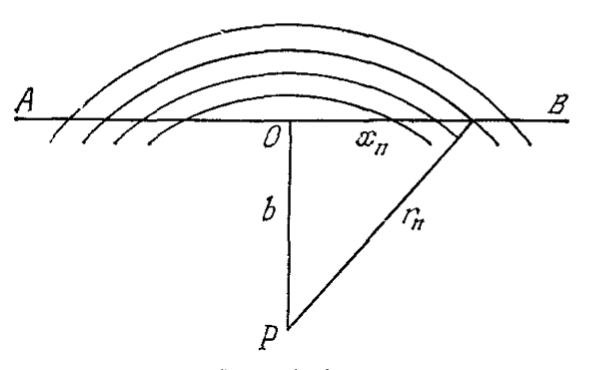
\includegraphics{31_1}
	\caption{Иллюстрация для зон Шустера}
\end{figure}

Проведем цилиндрические коаксиальные поверхности, ось которых проходит через точку $P$ перпендикулярно к плоскости рисунка, радиусы которых равны $b$, $b + \lambda/2$, $b + \lambda$ и т.д. Тогда волновой фронт разобьется на прямоугольные зоны, которые называются \textbf{зонами Шустера}. Центральную зону условимся считать сразу за две (одна слева от $O$, другая справа от $O$). В таком случае:

\begin{equation*}
	r_n^2 = b^2 + x_n^2, \quad r_{n-1}^2 = b^2 + x_{n-1}^2 \qrq r_n^2 - r_{n-1}^2 = x_n^2 - x_{n-1}^2
\end{equation*}

Приближенно мы получим:

\begin{equation*}
	r_n^2 - r_{n-1}^2 = (r_n - r_{n-1})(r_n + r_{n-1}) = 2 b (\lambda / 2) = b \lambda
\end{equation*}

Отсюда получаем рекуррентное соотношение:

\begin{equation*}
	x_n^2 - x_{n-1}^2 = b \lambda
\end{equation*}

С учетом того, что $x_0$ = 0, мы можем получить все $x_n$:

\begin{equation*}
	x_1 = \sqrt{b \lambda}, \quad x_2 = \sqrt{2 b \lambda}, \quad ..., \quad x_n = \sqrt{n b \lambda}
\end{equation*}

В таком случае ширины последовательных зон Шустера:

\begin{equation*}
	\sqrt{b \lambda}, \quad (\sqrt{2} - 1) \sqrt{b \lambda}, \quad (\sqrt{3} - \sqrt{2})\sqrt{b \lambda}
\end{equation*}

Согласно принципу Гюйгенса-Френеля волновое поле в точке $P$ представляется интегралом:

\begin{equation*}
	E_p = \int \frac{1}{r r'} e^{i \Phi(R)} d F
\end{equation*}

Заметная интенсивность наблюдается лишь при малых углах дифракции, поэтому изменениями $r r'$ можно пренебречь. Если рассматривать относительное распределение интенсивности, можно положить $r r' = 1$. В плоскости волнового фронта мы можем положить $\Phi = \omega t - k r$ (здесь мы проведем переобозначение: $r'$ из старой формулы теперь становится $r$).

Примем фазовый фронт за плоскость $XY$, начало координат положим в точке $O$. Тогда $r^2 = b^2 + (x^2 + y^2)$. Тогда $r - b = (x^2 + y^2) / (2 b) + ...$. Члены высших порядков можно отбросить (даже если вклад порядка $\pi$), т.к. они, как будет потом видно из формы полученной нами спирали, будут производить лишь незначительные смещения дифракционных максимумов и минимумов. Кроме того, высшие дифракционные максимумы и минимумы следуют друг за другом так часто, что для их реального осуществления требуются источники высокой степени монохроматичности. В противном случае они сольются в равномерный освещенный фон. Отбросим все фазовые множители, не влияющие на относительное распределение интенсивности светового поля. Тогда поле в точке $P$ оказывается равным:

\begin{equation*}
	E_p = \int \int e ^{- i k (x^2 + y^2) / (2 b)} dx dy
\end{equation*}

Пусть по оси $Y$ поле простирается довольно далеко. Тогда по $y$ можно интегрировать в пределах $-\infty, \infty$. От этого появится некоторый постоянный член, который нам не особо интересен. Интегрирование по оси $x$ произведем от 0, а верхний предел будем считать переменным ($x$). Вместо $x$ тогда введем новую переменную $s$ такую, что:

\begin{equation*}
	\frac{k x^2}{b} = \pi s^2
\end{equation*}

В таком случае получатся интегралы:

\begin{align*}
	E_p &= \int \limits_0^s e^{- i \pi s^2 / 2} d s \\
	E_p^* &= \int \limits_0^s e^{i \pi s^2 / 2} d s 
\end{align*}

Для изображения колебаний можно пользоваться любым из выражения. Для построения спирали будем пользоваться вторым выражением (в комплексной форме). В прямоугольных координатах мы в таком случае получим:

\begin{align*}
	X(s) = \int\limits_0^s \cos\left(\frac{\pi s^2}{2}\right) d s \\
	Y(s) = \int\limits_0^s \sin\left(\frac{\pi s^2}{2}\right) d s
\end{align*}

Данные интегралы называются \textbf{интегралами Френеля}. Из них видно, что получаемая кривая должна быть симметрична относительно начала координат.

Чтобы найти фокусы спирали, положим $s \rightarrow \infty$. Тогда окажется:

\begin{equation*}
	X_F = Y_F = \frac{1}{2}, \quad X_{F'} = Y_{F'} = -\frac{1}{2}
\end{equation*}

Для того, чтобы пользоваться спиралью, необходимо уметь находить $s$. Зная ширину первой зоны Шустера $\sqrt{\lambda b}$ мы далее получаем, что:

\begin{equation*}
	s = x \sqrt{\frac{2}{\lambda b}}
\end{equation*}

Для полноты картины необходимо получить графическую интерпретацию $s$. Из уравнения спирали в комплексной форме получаем для дифференциала дуги спирали:

\begin{equation*}
	\left|e^{i \pi s^2 / 2} d s\right| = |ds|
\end{equation*}

Отсюда следует, что параметр $s$ определяет длину дуги спирали, отсчитываемую от начала координат $O$.

\subsection{Дифракционная картина от прямолинейного края экрана}

Где бы ни находилась точка $P$, для нее всегда оказывается открытым первый край волнового фронта. На спирали колебание представляется вектором $\overrightarrow{M_n F}$. Если мы теперь будем двигать точку $M_n$ по спирали Корню, то мы получим распределение амплитуд и интенсивностей колебаний света по экрану. Спираль Корню представлена на рисунке ниже.

\begin{figure}[H]
	\centering
	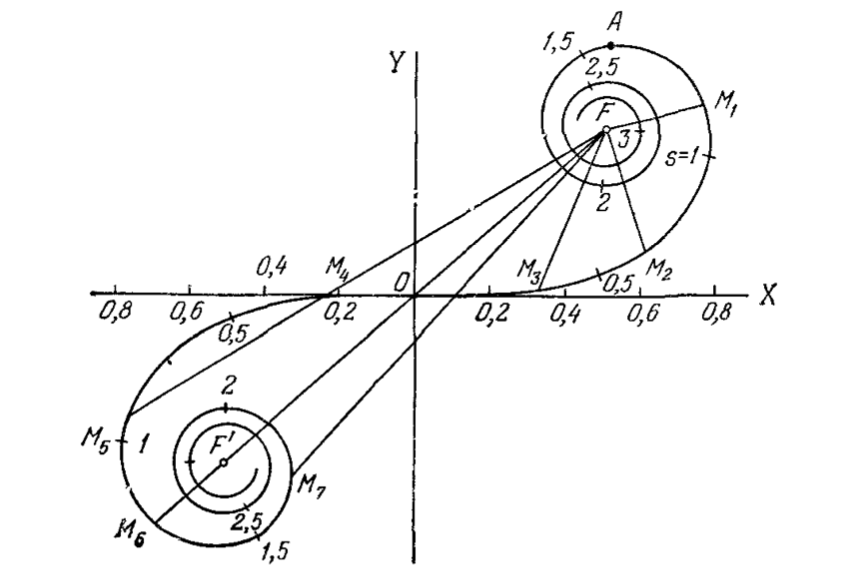
\includegraphics{31_2}
	\caption{Спираль Корню для дифракции на прямоугольном краю экрана.}
\end{figure}

Положим $a_0 = |F F'|$, $I_0 = a_0^2$ Когда точка наблюдения находится на границе геометрический тени, ей соответствует колебание, которое представимо вектором $\longrightarrow{OF} = 1/2 \longrightarrow{F'F}$. Этому соответствует амплитуда $1/2 a_0$ и, соответственно, интенсивность $1/4 I_0$. При перемещении точки в освещенную область, точка $M_n$ будет смещаться дальше по спирали и мы получим следующий график:

\begin{figure}[H]
	\centering
	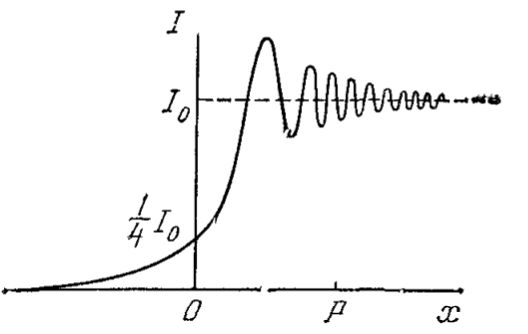
\includegraphics{31_3}
	\caption{Зависимость интенсивность от положения точки наблюдения при дифракции на прямолинейном краю экрана.}
\end{figure}






	
	\newpage
	
	\input{TeX_files/32.tex}
	
	\newpage
	
	\section{Дифракционная решетка. Амплитудные и фазовые дифракционные решетки. Дифракционная решетка как спектральный прибор. Разрешающая способность дифракционной решетки. Критерий Рэлея}

\subsection{Дифракционная решетка}

\Def{Дифракционная решетка} --- спектральный прибор,предназначенный для разложения света в спектр и измерения длин волн. Ширину щели как правило обозначают $a$, ширину непрозрачной части экрана между щелями --- $b$. Величина $d = a + b$ --- период решетки. Дифракционная картина наблюдается по методу Фраунгофера.

\begin{figure}[H]
	\centering
	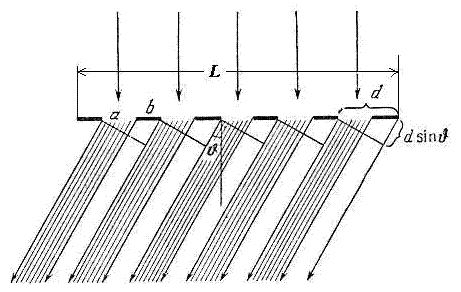
\includegraphics{33_1}
\end{figure}

Здесь угол $\upsilon$ --- угол дифракции.

Разность хода между вторичными волнами, исходящими из соседних щелей $d\sin{\upsilon}$, а разность фаз $\delta = k d\sin{\upsilon}=\frac{2\pi}{\lambda}d\sin{\upsilon}$

Если $E_i$ -- вклад в поле, измеренное в точке наблюдения от $i$-той щели, то:

\begin{align*}
	E_1 &= a\frac{\sin{\alpha}}{\alpha}, \alpha = \frac{kb\sin{\upsilon}}{\upsilon}\\
	E_2 &= E_1 e^{(-i\delta)}\\
	E_3 &= E_1 e^{(-2i\delta)}, E_N = E_1 e^{(-(N-1)i\delta)}
\end{align*}

Для N щелей поле представляется суммой:

\begin{equation*}
	E = E_1[1+e^{(-i\delta)} + ... + e^{(-(N-1)i\delta)}] = E_1\frac{1-e^{(-Ni\delta)}}{1-e^{(-i\delta)}} = E_1\frac{\sin{N\delta/2}}{\sin{\delta/2}}e^{-i(N-1)\delta/2}
\end{equation*}

Тогда интенсивность выражается через интенсивность одной щели:

\begin{equation*}
	I = I_1[\frac{\sin{N\delta/2}}{\sin{\delta/2}}]^2
\end{equation*}

Для особых случаев $\upsilon=0$ и $d\sin{\upsilon}=m\lambda$ формулы дают следующие результаты:

\begin{equation*}
	A=A_1 N, I = I_1 N^2
\end{equation*}

В направлениях, определяемых этим условием,получаются главные максимумы. Интенсивность в соответствующих точках превышает исходную в $N^2$ раз. 

\Def{Условие главных максимумов}: $d\sin{\upsilon}=m\lambda$

Здесь целое число $m$ --- порядок спектра.

Однако при некоторых значениях m максимум может не возникнуть, например, если он максимум одной щели накладывается на минимум другой. При a = b каждый второй максимум не будет виден и условие главных максимумом будет совпадать с условием дифракционного минимума одной щели: $d = a+b = 2a, 2a \sin{\upsilon} = 2n \lambda$

\Def{Условие дифракционного минимума одной щели}: $a \sin{\upsilon} = (m + 1/2) \lambda$ 

Для поиска дифракционных минимумов посмотрим, при каком условии формула интенсивности зануляется:

\begin{equation*}
 \begin{cases}
   \sin\left(\dfrac{N \delta}{2}\right) = 0 \\
	\sin\left(\dfrac{\delta}{2}\right) \ne 0
 \end{cases}
\end{equation*}

\begin{equation*}
	N\delta/2=(Nm+p)\pi, \qlrq d\sin{\upsilon}=(m+\frac{p}{N})\lambda, p = 1, 2, ..., N-1
\end{equation*}

Между двумя соседними минимума будут возникать второстепенные максимумы. Между двумя главными максимумами располагаются $N-1$ минимумов и $N-2$ второстепенных максимумов.

Найти величину $\delta$ можно найти по приближенной формуле:

\begin{equation*}
	N\delta/2=\frac{(Nm+p)\pi}{2}+\frac{(N(m+1)+p)\pi}{2} \qlrq \delta/2=(m+\frac{2p+1}{2N})\pi
\end{equation*}

Дифракционная картина выглядит следующим образом:

\begin{figure}[H]
	\centering
	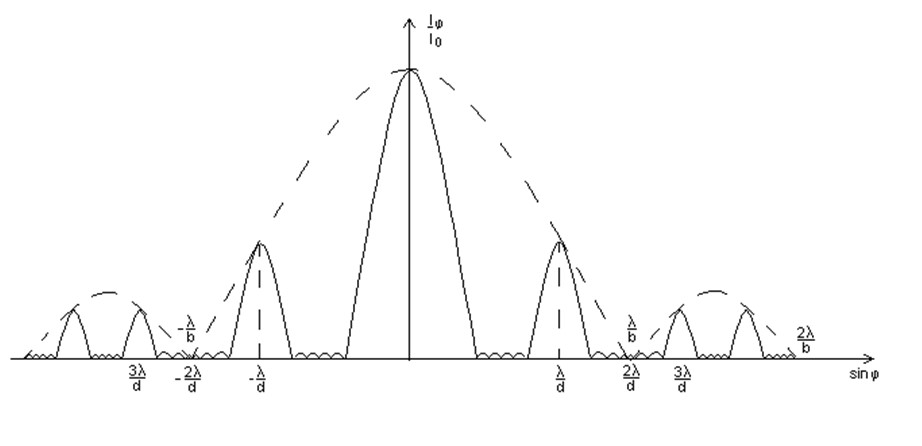
\includegraphics[width=\textwidth]{33_2}
\end{figure}

Если волна падает под углом, разность хода между соседними пучками $d(\sin{\upsilon} - \sin{\upsilon_0})$. Характер дифракционной картины сохранится, но условия минимумов и максимумов изменятся:

\begin{itemize}
	\item \textbf{Условие главных максимумов}:
	
	\begin{equation*}
		d(\sin{\upsilon}-\sin{\upsilon_0})=m\lambda
	\end{equation*}
	
	\item \textbf{Условие дифракционного минимума одной щели}:
	
	\begin{equation*}
		d(\sin{\upsilon}-\sin{\upsilon_0})=(m+p/N)\lambda
	\end{equation*}
\end{itemize}

Дифракционную решетку используют для измерения длины волны.

\subsection{Амплитудные и фазовые дифракционные решетки}

\Def{Амплитудная решетка} Решетка, вносящая периодические изменения в амплитуду волны, не влияя на ее фазу.
Примером является рассмотренная выше решетка.

\Def{Фазовая решетка} Решетка, вносящая  периодические изменения в фазу волны, не влияя на ее амплитуду.

\begin{figure}[H]
	\centering
	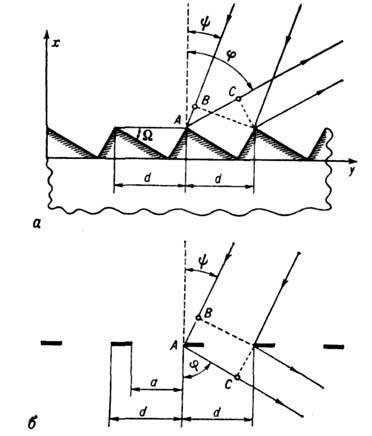
\includegraphics[scale=0.5]{33_3}
	\caption{а) Фазовая решетка; б) Амплитудная решетка}
\end{figure} 

\subsection{Дифракционная решетка как спектральный прибор}
Положение главных максимумов ненулевого порядка зависит от длины волны, значит, всякий сложный свет при прохождении через дифракционную решетку будет раскладываться в спектр:  отдельные монохроматические компоненты разделятся, отклонившись на разные углы. Дифракционные максимумы 1 порядка образуют спектр 1 порядка, затем образуется спектр 2, 3 порядка и т.д.

Спектр называется нормальным, если координата x, характеризующая положение спектральной линии, меняется линейно с длиной волны. Решетка дает нормальный спектр на малых углах.

\begin{figure}[H]
	\centering
	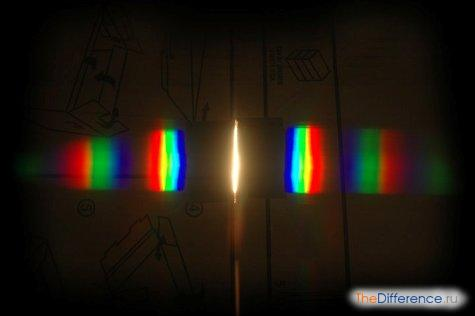
\includegraphics[scale=0.5]{33_4}
\end{figure} 

\subsection{Разрешающая способность дифракционной решетки}

\Def{Угловая дисперсия}: производная $\dfrac{d\upsilon}{d\lambda}=\dfrac{m}{d\cos{\upsilon}}=\dfrac{\sin{\upsilon}-\sin{\upsilon_0}}{\lambda\cos{\upsilon}}$. Не зависит от параметров решетки.

\Def{Дисперсионная область} Максимальная ширина спектрального интервала $\Delta\lambda$, при которой еще нет перекрытия спектров соседних порядков. Крайний случай --- правый конец спектра $m+1$ порядка для длины волны $\lambda$совпадает с левым концом спектра порядка $m$ для длины волны $\lambda'$. Тогда:

\begin{align*}
	d(\sin{\upsilon}-\sin{\upsilon_0})=m\lambda'=(m+1)\lambda\\
	\lambda'-\lambda=\Delta\lambda=\frac{\lambda}{m}
\end{align*} 

Большая дисперсия еще не говорит о том, что две спектральные линии воспринимаются при наблюдении как раздельные объекты,так как любой спектральный аппарат изображает линию как размытую полосу с собственными максимумами и минимумами(дисперсия).Чем более узкие спектральные линии, тем на меньшее расстояние надо их развести, чтобы "разрешить" их. Широкие и сильно размытые линии дадут дифракционную картину одной спектральной линии.
 
\Def{разрешающая способность аппарата}: величина $R=\dfrac{\lambda}{\delta\lambda}$ называется разрешающей способностью аппарата, где $\delta\lambda$ --- наименьшая разность длин волн двух спектральных линий, при которой спектральный аппарат разрешает их.

\subsection{Критерий Рэлея}

Критерий спектрального разрешение дифракционной решетки. Спектральные линии с близкими длинами волн называются разрешенными, если главный максимум дифракционной картины совпадает с первым дифракционным минимумом в том же порядке для другой длины волны. 

\begin{align*}
	d(\sin{\upsilon}-\sin{\upsilon_0})=m\lambda'=(m+\frac{1}{N})\lambda\\
	\delta\lambda=\frac{\lambda}{Nm} \qrq R=Nm
\end{align*}

\begin{figure}[H]
	\centering
	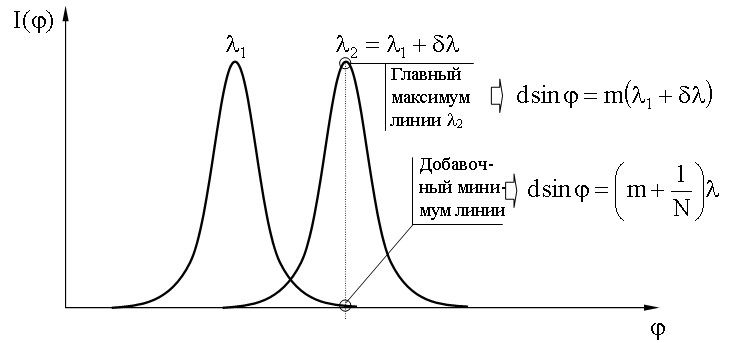
\includegraphics[width=\textwidth]{33_5}
\end{figure} 

Такого вида картина интенсивности позволяет явно увидеть 2 полосы вместо 1.

	
	\newpage
	
	\section{Спектральный прибор и его основные характеристики - апаратная функция, линейная дисперсия, разрешающая способность и область дисперсии.}





\subsection{Дисперсионная область}




Область дисперсии - максимальная ширина спектрального интервала $\Delta \lambda$, при которой спектры соседних порядков еще не перекрываются. Если спектры начали накладываться друг на друга, данный прибор не позволяет исследовать данный интервал $\Delta \lambda$.

\begin{figure}[h!]
    \centering
    \includegraphics[scale=0.25]{34_1}
    \caption{Качественный вид дифракционной картины, получаемой дифракционной решеткой, на которую падает свет с конечной шириной спектра $\Delta\lambda$.}
    \label{fig:my_label}
\end{figure} 

Найдем условие, при котором начинается перекрытие. Возьмем спектральный диапазон $(\lambda,\lambda'), $  $\lambda' = \lambda  + \Delta \lambda.$  Главный максимум $m$-ого порядка для границы спектра $\lambda' $ имеет такое направление, что

\begin{equation*}
    d\sin\theta = m\lambda'.
\end{equation*}

Максимум $(m+1)$-ого порядка для границы спектра $\lambda$ должен распространяться под тем же углом, так что

\begin{equation*}
    d\sin\theta = (m+1)\lambda.
\end{equation*}

\begin{equation*}
    (m+1)\lambda = m\lambda' \Rightarrow m\Delta\lambda = \lambda \Rightarrow \Delta\lambda = \frac{\lambda}{m}.
\end{equation*}

Таким образом, спектры $m$-ого и $(m+1)$-ого порядка не перекрываются, если ширина спектрального диапазона достаточно мала:

\begin{equation*}
    \Delta \lambda \leq \frac{\lambda}{m}
\end{equation*}
\subsection{Угловая дисперсия}

Угловая дисперсия дифракционного прибора - это величина, определяемая равенством

\begin{equation*}
    D = \frac{d\theta}{d\lambda}
\end{equation*}

Она определяет угловое расстояние $d\theta$ между спектральными линиями, отстоящими по длине волны на $d\lambda$:
\begin{equation*}
   \Delta \theta \approx D \Delta \lambda
\end{equation*}

Например, для дифракционной решетки имеем
\begin{equation*}
    \sin \theta = m\frac{\lambda}{d}  \Rightarrow D = \frac{m}{d\cos\theta}
\end{equation*}

В частности, для малых углов дифракции

\begin{equation*}
    D = \frac{m}{d}
\end{equation*}

\subsection{Линейная дисперсия}

Линейная дисперсия - это расстояние между разрешаемыми линиями спектра на экране, на котором рассматривается дифракционная картина. 

\begin{figure}[h!]
    \centering
    \includegraphics[scale=0.25]{34_2}
    \caption{Волны, отвечающие разным спектральным компонентам, отображаются с помощью линзы на экране в разные точки}
    \label{fig:my_label}
\end{figure} 


Отображая спектральные компоненты $\lambda$ и $\Delta \lambda$ в фокальной плоскости линзы, получаем линейное расстояние $\Delta l$ между ними на экране. Формально линейная дисперсия определяется равенством

\begin{equation*}
    D_{\text{лин}} = \frac{dl}{d\theta}
\end{equation*}

Поскольку $ dl = f\cdot d\theta$, то

\begin{equation*}
    D_{\text{лин}} = f \cdot D \approx \frac{fm}{d}
\end{equation*}

(Здесь использовано $D = \frac{m}{d}$ для дифракционной решетки)
\subsection{Разрешающая способность}

Разрешающая способность спектрального прибора - это величина, определяемая равенством

\begin{equation*}
    R = \frac{\lambda}{\Delta \lambda}, \text{где}
\end{equation*}

$\Delta \lambda$ - минимальная разность длин волн двух спектральных линий, которые воспринимаются раздельно.

\begin{figure}[h!]
    \centering
    \includegraphics[scale=0.25]{34_3}
    \caption{Дифракционные пятна от двух компонент спектра, $\theta_d - $угловой радиус главного дифракционного максимума}
    \label{fig:my_label}
\end{figure} 


В качестве примера найдем разрешающую способность дифракционной решетки. Используем критерий Рэлея(см.рисунок). Пусть решетка имеет $N$ штрихов. Выберем главный максимум $m-$ого порядка для компоненты $\lambda$. Направление на первый дифракционный минимум даетмя равенством

\begin{equation*}
    d\sin \theta_d = \left(m + \frac{1}{N}\right) \lambda
\end{equation*}

Согласно критерию Рэлея компоненты считаются разрешенными, если это же направление соответствует главному дифракционнуму максимуму для второй компоненты $\lambda + \Delta \lambda$:

\begin{equation*}
    d\sin \theta_d = m(\lambda + \Delta\lambda)
\end{equation*}

\begin{equation*}
   \left(m + \frac{1}{N}\right) \lambda = m(\lambda + \Delta \lambda) \Rightarrow \Delta \lambda = \frac{\lambda}{mN}
\end{equation*}

Таким образом, получим разрешающую способность дифракционной решетки:

\begin{equation*}
   R = \frac{\lambda}{\Delta \lambda} = mN
\end{equation*}





	
	\newpage
	
	\input{TeX_files/35.tex}
	
	\newpage
	
	\section{Роль дифракции в приборах, формирующих изображение. Критерий Рэлея (применительно к формированию изображений). Дифракционный предел разрешения телескопа и микроскопа.}

Из-за наличия во Вселенной дифракции Фраунгофера на круглом отверстии, вместо точки при фокусировке света мы получаем небольшое пятнышко, которое называется \textbf{пятном (диском) Эйри}. Его радиус можно рассчитать по следующей формуле:

\begin{equation*}
	\rho_{a} = 1.22 \frac{\lambda}{D} F	
\end{equation*}

Здесь $\lambda$ --- длина волны наблюдаемого излучения, $D$ --- диаметр линзы, $F$ --- ее фокусное расстояние.

Пусть мы наблюдаем некоторый объект, который находится на главной оптической оси. Тогда и его изображение будет находиться там же. Пусть теперь у нас добавляется еще один объект, который находится от первоначального на некотором (небольшом) угловом расстоянии $\psi$. Пятно Эйри от этого объекта в таком случае будет находиться на таком же угловом расстоянии от исходного пятна, а линейное расстояние тогда будет равно $l = F \psi$. 

Для того, чтобы понять, возможно ли эти два объекта разрешить, был введен так называемый \textbf{критерий Рэлея}, который говорит, что минимальное расстояние между объектами, на котором их можно разрешить, оказывается таким, что первый минимум пятна Эйри от одного объекта приходится на нулевой максимум пятна Эйри другого.

С учетом имеющейся у нас формулы для радиуса пятна Эйри мы получим:

\begin{equation*}
	\psi_{min} F = 1.22 \frac{\lambda}{D} F \qrq \boxed{\psi_{min} = 1.22 \frac{\lambda}{D}}
\end{equation*}

Рассмотрим теперь микроскоп. Предположим, что предмет у нас лежит в какой-то среде с показателем преломления $n$ (так делается, например, в диффузионных микроскопах); по другую сторону линзы у нас, соответственно, воздух, с показателем преломления $n_{air} = 1$. Как уже было сказано ранее, от каждой точки предмета будет получаться не точечное изображение, а пятно Эйри. Введем углы $u_1$ и $u_2$ (см. рисунок). Угол $u_1$ называется апертурным углом объектива.

\begin{figure}[H]
	\centering
	\includegraphics[width=\linewidth]{36_1}
\end{figure}

Как видно из рисунка, верно следующее:

\begin{equation*}
	\frac{D}{L} \approx 2 u_2 \approx 2 \sin u_2
\end{equation*}

Согласно Аббе, идеальный с точки зрения геометрии микроскоп подчиняется следующему условию (\textbf{условие синусов Аббе}):

\begin{equation*}
	l_1 n_1 \sin u_1 = l_2 n_2 \sin u_2 \qrq l_1 n \sin u_1 = l_2 \frac{D}{2L}
\end{equation*}

Здесь $l_1$ и $l_2$ есть линейные размеры предмета и изображения соответственно.

Ну и с учетом критерия Рэлея, который в данном случае удобно сформулировать как "линейный размер изображения должен получаться не меньше радиуса пятна Эйри", мы получим:

\begin{equation*}
	l_{2 min} = \rho_a = l_{1 min} \frac{2 L n\sin u_1}{D} = 1.22 \frac{\lambda}{D} L \qrq l_{1 min} = 0.61 \frac{\lambda}{n\sin u_1}
\end{equation*}

Выражение $n \sin u_1$ в знаменателе называют \textbf{числовой апертурой микроскопа}.
	
	\newpage
	
	\input{TeX_files/37.tex}
	
	\newpage
	
	\input{TeX_files/38.tex}
	
	\newpage
	
	
\section{Физические принципы голографии. Голограмма Д. Габора, голограмма Ю.Н. Денисюка.}


\textit{Голография} - это метод точной записи волновый полей с учетом амплитуды и фазы.

\medskip 

Для записи голограммы помимо \textit{предметной волны} от фотографируемого объекта используется еще одна волна, называемая \textit{опорной}. На фотографии записывается результат их интерференции, в результате чего записывается информация о фазе предметной волны (относительно опорной). При освещении голограммы восстанавливающей волной, которая должна быть идентична опорной, получаем обратно предметную волну.



\begin{figure}[h!]
    \centering
    \includegraphics[scale=0.25]{holo1.PNG}
    \caption{Запись голограммы}
    \label{fig:my_label}
\end{figure} 



\begin{figure}[h!]
    \centering
    \includegraphics[scale=0.25]{holo2.PNG}
    \caption{Восстановление голограммы}
    \label{fig:my_label}
\end{figure} 
\newpage


\subsection{Голограмма Габора}

Если опорная волна падает по нормали на фотопластинку в том же направлении, что и предметная волна, реализуется \textit{схема Габора}. (Схема описана выше.)
\subsection{Голограмма Денисюка}

Если предметная и опорная волна идут навстречу друг другу, то реализуется \textit{схема Денисюка}. Эта схема используется при записи толстых (объемных) голограмм.

С помощью метода Денисюка получаются трехмерные, объемные голограммы на пластинках с толстослойной эмульсией.

Опорная плоская монохроматическая волна от лазера падает на фотопластинку со стороны стекла. Пройдя через фотопластинку, она освещает голографируемый предмет. Волна, рассеянная предметом, распространяется навстречу опорной волне, интерферируя с ней в толще фотоэмульсии. Интерференционная картина представляет стоячик волны, на который наложен причудливый узор мелких деталей из максимумов и минимумов, так как среди интерферирующих волн только опорная волна является плоской. Проявленная и отфиксированная фотопластинка и будет объемной голограммой Денисюка. Она состоит как бы из нескольких десятков поверхностных голограмм, расположенных в толще эмульсии.

\medskip


Восстановление предметной волны производится расходящимся пучком белого света. Каждый слой выделившегося серебра, действуя подобно двухмерной голограмме, дает слабые мнимое и действительное изображения предмета. При многолучевой интерференции происходит усиление тех волн, длина которых равна длине волны излучения лазера, в тех направлениях, в которых разность фаз между волнами от соседних слоев серебра равна $2\pi$. В результате возникают изображения того же цвета, что и цвет луча лазера. Остальные изображения гасят друг друга при интерференции.

\medskip

Таким образом, голограмма производит монохроматизацию белого света, которым она освещается. Конечно, такая монохромати-зация сравнительно невысокая, из-за незначительного числа отложившихся слоев серебра и связанной с этим небольшой спектральной разрешающей способности голограммы. Кроме того, цвет изображения может существенно отличаться от цвета излучения лазера. Это связано с изменением расстояний между слоями почернения при проявлении, фиксировании и сушке фотопластинки.

\medskip

Метод Денисюка, подобно трехцветной фотографии, позволяет получать изображения предметов в натуральных цветах. Для этого на одной и той же фотопластинке получают голограмму предмета с помощью трех лазеров, излучения которых имеют различные длины волн. Последние подбираются так, чтобы при смешении они наиболее совершенно воспроизводили цвет предмета. Такая голограмма действует как три голограммы, дающие при освещении белым светом совмещенные изображения предмета в трех цветах. При этом цвет изображения кажется глазу таким же, как и цвет самого предмета.

	
	\newpage
	
	\input{TeX_files/40.tex}
	
	\newpage
	
	\section{Зависимости показателя преломления и коэффициента поглощения от частоты. Дисперсионная формула Зелмеера. Фазовая и групповая скорости. Формула Рэлея.}
\subsection{Зависимости показателя преломления и коэффициента поглощения от частоты}
На некоторых экспериментах люди стали замечать зависимость показателя преломления от длины волны(частоты) падающего света, знаменитое разделение пучка посредством призмы:
\begin{figure}[h]\label{qr}
	\center{\includegraphics[scale=0.25]{41_1.jpg}}
	\caption{Иллюстрация дисперсии}
	\label{fig:image}
\end{figure}


Первая формула, которая описывала это называется \textbf{формулой Коши}(нормальный ход дисперсии), она представляет рял по обратным четным степеням длины волны:
\begin{equation}
n(\lambda) = a + b/\lambda^2 + c/\lambda^4 + ...
\end{equation}
Эта формула абсолютно эмпирическая и поэтому числовые коэффициенты должны быть найдены в ходе эксперимента.

Дальше про микроскопическую теорию: запишем показатель преломления через диэлектрическую проницаемость: $n = \sqrt{\varepsilon}$, также поговорим о специфике задачи: атом в электрическом поле это диполь с дипольным моментом равным : $p = r\cdot e$. Тогда запишем уравнение движения атомного осциллятора:
\begin{equation}
m \ddot{r} = eE - kr - \gamma \dot{r}
\end{equation}
где второе слагаемое определяет удерживающую силу, а третье диссипацию энергии. Немного преобразовав (заменив радиус вектор на дипольный момент, а также умножив на e/m ) получим: 
\begin{equation}
p + \gamma \dot{p} + \omega_{0}^2 p = \frac{e^2}{m}E_0 e^{-i\omega t}
\end{equation}
Где расписана плоская волна, и в ней мы считаем, что заряд локализован в окрестности начала координат, а также скорость приобретаемая при колебаниях значительно меньше скорости света, поэтому действием магнитного поля можно пренебречь. Такое уравнение решается экспоненциальным анзацем, поэтому решение имеет вид:
\begin{equation}
p=\frac{e^{2} E_{0}}{m} \cdot \frac{1}{\left(\omega_{0}^{2}-\omega^{2}\right)-(i \gamma \omega)} e^{-i \omega t}
\end{equation}
Дальше вспомним определение тела --- это среда состоящая из диполей, а поэтому мы зная некоторые соотношения между основными электромагнитными характеристиками получить :
\begin{equation}
D = E + 4 \pi P = E + 4 \pi N p = \varepsilon E
\end{equation}
Откуда несложно выражается диэлектрическая проницаемость:
\begin{equation}\label{eps}
\varepsilon=1+\frac{4 \pi N e^{2}}{m} \cdot \frac{1}{\left(\omega_{0}^{2}-\omega^{2}\right)-i \gamma \omega}
\end{equation}
Вспоминаем, что показатель преломления --- это корень из эпсилон, а поэтому становиться понятно, что во--первых легитимно существование мнимого показателя преломления, а во--вторых, вследствие многозначности корня мы получаем много ветвей нашего показателя преломления.


Также можно без труда заметить, что имеется резонансный характер, а значит без трения и в ситуации совпадения внешней и внутренней частот будет наблюдаться резонанс.

Теперь распишем показатель преломления: $\hat{n} = n(1-i\varkappa)$, где $\varkappa$ -- коэффициент поглощения. а дальше используя выражение \eqref{eps} получим два выражения, определяющие зависимости из названия главы: 
\begin{equation}
n^{2}\left(1-\varkappa^{2}\right)=1+4 \pi \frac{e}{m} N_{0} \frac{f\left(\omega_{0}^{2}-\omega^{2}\right)}{\left(\omega_{0}^{2}-\omega^{2}\right)^{2}+\omega^{2}(\gamma / m)^{2}}
\end{equation}
\begin{equation}
2 n^{2} \varkappa=4 \pi \frac{e}{m} N_{0} \frac{f(\gamma / m) \omega}{\left(\omega_{0}^{2}-\omega^{2}\right)+\omega^{2}(\gamma / m)^{2}}
\end{equation}
где первое кривая дисперсии, а вторая кривая поглощения (абсорбции): 
\begin{figure}[h]\label{qr}
	\center{\includegraphics[scale=0.25]{41_2.jpg}}
	\caption{ Кривая дисперсии (сплошная) и абсорбции (пунктирная)}
	\label{fig:image}
\end{figure}


Если также учесть взаимодействие с молекула среды(вот так $E^{\prime}=E+\frac{4 \pi}{3} P$) получаем формулу Лоренц - Лорентца:
\begin{equation}
\frac{n^{2}-1}{n^{2}+1}=N_{0} \frac{4 \pi e^{2} f}{3 m\left(\omega_{0}^{2}-\omega^{2}\right)}
\end{equation}

\subsection{Дисперсионная формула Зельмейера}

Если полос поглощения(резонансов) много, тогда мы получаем (пренебрегая затуханием) и суммируем по всем частотам переходов получаем:
\begin{equation}
n^{2}=1+4 \pi N_{0} \sum \frac{f_{i} e_{i}^{2}}{m_{i}} \frac{1}{\left(\omega_{0 i}^{2}-\omega^{2}\right)}
\end{equation}
Где через $f_i$-- обозначена сила.
\begin{figure}[h]\label{qr}
	\center{\includegraphics[scale=0.25]{41_3.jpg}}
	\caption{ Кривая дисперсии при нескольких резонансах}
	\label{fig:image}
\end{figure}
\subsection{Фазовая и групповая скорость, формула Рэлея}
\Def{Фазовая скорость} --- скорость распространения волнового фронта: $V = \omega/k=c/n$, в вакууме совпадает со скоростью света.

Теперь попробуем осознать, что такое групповая скорость: рассмотрим движения волнового пакета с шириной частот $2\delta \omega \ll \omega_0$, распишем два закона движения волн, для двух крайних частот спектра: 
\begin{equation}
y_{1}=a \sin \left(\omega_{1} t-k_{1} x\right) \quad \text { и } \quad y_{2}=a \sin \left(\omega_{2} t-k_{2} x\right), \quad \omega_{1,2}= \omega_0 \pm \delta \omega
\end{equation}

Просуммируем и преобразуем тригонометрическими формулами:

\begin{equation}
y=y_{1}+y_{2}=\underbrace{2 a \cos (t \delta \omega-x \delta k)}_{A} \sin \left(\omega_{0} t-k_{0} x\right)
\end{equation}
Выделим на импульсе точку, где $\boldsymbol{A}$ максимально. Скорость перемещения этой
точки характеризует скорость распространения импульса. Таким образом,
скорость импульса (группы), которую, по Рэлею, называют \Def{групповой
скоростью}, есть скорость перемещения амплитуды, $a,$ следовательно
энергии, переносимой движущимся импульсом.
\begin{equation}
A=\text {const} \Rightarrow t \delta \omega-x \delta k=\text {const} \Rightarrow \delta \omega d t-\delta k d x=0
\end{equation}
Отсюда найдем, что групповая скорость равна: 
\begin{equation}
u = \frac{dx}{dt} = \frac{\delta \omega}{\delta k} = \frac{d\omega}{dk}
\end{equation}
Выразив фазовую скорость через волновой вектор и используя определение длины волны, несложно получить \Def{формулу Рэлея}:
\begin{equation}
u=\frac{d \omega}{d k}=\frac{d(V k)}{d k}=V+k \frac{d V}{d k}, k=\frac{2 \pi}{\lambda}
\end{equation}
\begin{equation}
\fbox{$u=V-\lambda \dfrac{d V}{d \lambda}$}
\end{equation}
Можно немного преобразовать и получить:
\begin{equation}
u=\frac{c}{n+\omega \cdot d n / d \omega}
\end{equation}


Если говорить о геометрическом смысле фазовой и групповой скорости нетрудно получить, что 
\begin{figure}[h]\label{qr}
	\center{\includegraphics[scale=0.25]{41_4.jpg}}
	\caption{ $\tan\alpha$ --- фазовая скорость, $\tan\beta$ --- групповая скорость}
	\label{fig:image}
\end{figure}

	
	\newpage
	
	\section{Тепловое излучение. Излучательная и поглощательная способности вещества и их соотношение. Модель абсолютно черного тела. Закон Кирхгофа.}

\textbf{Поглощение света.}

\theornp{Закон Бугера --- Ламберта --- Бера}{При распространении параллельного монохроматического пучка в поглощающей среде его интенсивность изменяется по закону $$I = I_0 e^{-\alpha d },$$ где $I_0$ --- интенсивность падающего пучка, $d$ --- ширина поглощаюего образца, $\alpha$ --- коэффициент поглощения.}

Чтобы исключить влияние коэффициента отражения $R$, нужно произвести опыты с образцами разной толщины. Тогда отношение интенсивностей равно $$I_1\setminus I_2 = e^{\alpha(d_2-d_1)}, \mbox{где } \alpha = \alpha(\omega)$$

\theornp{Закон Бера}{Поглощающая способность молекулы не зависит от влияния окружающих молекул.$$\alpha = Ac, \ I = I_0e^{-Acd}, \ A = \const$$}

Если имеется ряд полос поглощения (например, в парах натрия), то вблизи них коэффициент преломления веде себя следующим образом:
$$\tilde{n} = n(1 - i\chi) \Rightarrow \alpha = \frac{4\pi}{\lambda_0}n\chi.$$
\begin{figure}[H]
	\centering
	\includegraphics*[width=\textwidth]{Na}
\end{figure}
\newpage
\textbf{Тепловое излучение.}

\theornp{Правило Прево}{При установлении теплового равновесия в изолированной системе для каждого тела должно соблюдаться равенство между количеством испускаемой и поглощаемой им в единицу времени энергии. Если тела поглощают разные количества энергии, то и испускание должно быть различно.}

\begin{figure}[H]
	\centering
	\includegraphics*[width=0.4\textwidth]{T2}
\end{figure}

a) Тарелка имеет темный узор.
б) При нагревании темные области излучают сильнее.
$$$$
\textbf{Поглощательная способность.}

$A_\omega (T)$ --- отношение поглощённого потока $\Phi'$ к падающему $\Phi$.
$$A = \frac{d\Phi'}{d\Phi}$$
$A = 0$ --- абсолютно белое тело (например, мел).
$A = 1$ --- абсолютно черное тело (уголь, сажа).


\textbf{Абсолютно черное тело.}

\textit{Абсолютно черное тело} --- физическая абстракция; тело, поглощающее всё попадающее на него электромагнитное излучение во всех диапазонах и ничего не отражающее.

Абсолютно черное тело может испускать электромагнитное излучение любой частоты и визуально изменять цвет. Его спектр определяется только его \textbf{температурой}.

\textbf{Испускание света.}

Рассмотрим тело при температуре $Т$, испускающее с элементарной площадки $d\sigma$ поток излучения $d\Phi$ с частотами в диапазоне от $\omega$ до $\omega + d\omega$.

\begin{figure}[H]
	\centering
	\includegraphics*[width=0.3\textwidth]{Rad}
\end{figure}
$E_T(\omega), E_T(\lambda)$ --- \textbf{испускательная способность}, зависит от температуры излучающего тела и не зависит от темпераруты окружающих тел.
$$d\Phi = E_T(\omega)d\omega = E_T(\lambda)d\lambda$$
$$E(\omega)=E(\lambda)\frac{\lambda^2}{2\pi c}$$
Суммарное излучение $\Phi(T) = \int_{0}^{\infty}E_T(\omega)d\omega$

\theornp{Закон Кирхгофа}{Отношение испускательной и поглощательной способностей тела не зависит от природы тела.$$\frac{E_{\omega, T}}{A_{\omega, T}}=\epsilon_{\omega, T}$$}
$\epsilon_{\omega, T}$ --- универсальная для всех тел функция температуры и частоты. Она есть не что иное, как \textit{испускательная способность абсолютно черного тела}, так как для него $$\frac{E_{\omega, T}}{A_{\omega, T}}=\frac{\epsilon_{\omega, T}}{\alpha_{\omega, T}}=\epsilon_{\omega, T}, \ \alpha = 1.$$

Рассмотрим пример абсолютно черного тела с площадкой $d\sigma$ \textit{серого тела} ($0<\alpha <1$).
\begin{figure}[H]
	\centering
	\includegraphics*[width=0.3\textwidth]{T1}
\end{figure}

Такое тело вск еще не излучает. Как устанавливается динамическое равновесие при разности излучательной способности?
Оказывается, площадка $d\sigma$ частично отражает попадающий на нее свет (т.е. не поглощает его, как абсолютно черные стенки, а отражает), чем и поддерживает равенство излучаемого потока от всех элементарных площадок.
$$Ed\sigma = A\epsilon d\sigma, \ \epsilon d\sigma \mbox{ --- падающий поток,}$$
$$d\sigma[E + (1 - A)\epsilon] = \epsilon d\sigma, \mbox{где член } (1 - A) \mbox{ возникает из-за отражения.}$$

\begin{figure}[H]
	\centering
	\includegraphics*[width=0.3\textwidth]{T3}
\end{figure}
При тепловом равновесии рисунок становится неразличим, все области излучают одинаково.
	
	\newpage
	
	\section{Закон Стефана-Больцмана, формула смещения Вина. Формула Рэлея-Джинса. Ограниченность классической теории излучения. Элементы квантового подхода. Формула Планка. }


\subsection{Закон Стефана-Больцмана}
\textbf{Закон Стефана-Больцмана} - закон, связывающий поверхностную плотность излучения абсолютно черного тела (тела, которое при любой температуре поглощает все падающее на него излучение) с его температурой.
\begin{equation}
    P = \sigma T^4,
\end{equation}
где P - мощность излучения единицы поверхности абсолютно черного тела, T - температура, \(\sigma\)  - коэффициент пропорциональности, постоянная Стефана-Больцмана.


Эмпирически получен Стефаном, теоретически обоснован Больцманом методами статистической физики. Отметим, что закон говорит только об интегральной мощности излучения, но ничего не говорит о спектре. А вот о спектре скажет закон Рэлея-Джинса.


\subsection{Формула Рэлея-Джинса}
\textbf{Формула Рэлея-Джинса} - спектр (в данном случае закон распределения излучательной способности по частотам испускаемых волн) теплового излучения абсолютно черного тела при фиксированной температуре. При интегрировании этой формулы по всем частотам получается величина, пропорциональная полной мощности излучения. Закон получен Рэлеем и Джинсом теоретически в рамках классической теории. Записывается как:
\begin{equation}
\label{rj}
    B(\omega, T) = kT\frac{\omega^2}{4\pi^2 c^2},
\end{equation}
где \(B\) - яркость излучения в интервале частот от \(\omega\) до \(\omega + d\omega\), \(T\) - температура абсолютно черного тела, \(c\) - скорость света, \(k\) - постоянная Больцмана, \(\omega\) - циклическая частота световой волны, чей вклад в общее излучение мы смотрим.

\subsection{Ограниченность классической теории излучения}
Попробуем, собственно, проинтегрировать формулу Рэлея-Джинса (\ref{rj}) по всем частотам. Интергал, очевидно, расходится:
\begin{equation}
   P \sim \int_{0}^{\infty}  B(\omega, T) d\omega = \int_{0}^{\infty}  kT\frac{\omega^2}{4\pi^2 c^2}  d\omega \to \infty
\end{equation}
Иными словами, с точки зрения классической теории полная мощность теплового излучения единицы объема абсолютно черного тела при любой температуре бесконечно велика. Данный парадокс получил название ультрафиолетовой катастрофы, так как расходимость интеграла вызвана именно видом спектра излучения при больших частотах (см. рис. \ref{comparison})
\begin{figure}
    \centering
    \includegraphics{omparison.jpg}
    \caption{Сравнение законов излучения, о которых пойдет речь в билете}
    \label{comparison}
\end{figure}


\subsection{Элементы квантового подхода, формула Планка и формула смещения Вина}
На помощь по борьбе с парадоксами в классической теории снова приходят кванты. 


\textbf{Формула Планка} - полученный из квантово-статистических соображений закон распределения яркости теплового излучения по частотам при фиксированной температуре абсолютно черного тела. Записывается как:
\begin{equation}
\label{rj}
    B(\omega, T) = \frac{\hbar\omega^3}{4\pi^2 c^2}\frac{1}{\exp(\frac{\hbar\omega}{kT}) - 1},
\end{equation}
Обозначения те же, что и в формуле Рэлея-Джинса. При разложении экспоненты в знаменателе до первого порядка получится формула Рэлея-Джинса. То есть, при малых частотах излучения классическая теория еще работает. Это проиллюстрировано на рис. \ref{comparison} (за не-классический случай отвечает кривая, подписанная 'По Вину', почему так - будет понятно ниже).


\textbf{Закон смещения Вина} устанавливает зависимость частоты волны, на которой поток излучения энергии чёрного тела достигает своего максимума, от температуры чёрного тела. Дифференцируя формулу планка, приравнивая производную к нулю и отбрасывая 'скучные' решения в нуле и на бесконечности, получим запись закона Вина в виде трансцендентного уравнения:
\begin{equation}
    \frac{x\exp^x}{\exp^x - 1} = 5,
\end{equation}
где произведена замена \(x = \frac{\hbar \omega}{kT}\). Численно решив уравнение на \(x\) потом получим параметрическую связь \(\omega_{max}\) и \(T\):
\begin{equation}
    \omega_{max} = \frac{xkT}{\hbar}
\end{equation}
То есть, с ростом температуры линейно растет частота волны, соответствующей максимуму излучения, или, что то же самое, линейно падает длина волны. Это и иллюстрируется графиком \ref{win}.
\begin{figure}
    \centering
    \includegraphics[scale = 0.6]{win.png}
    \caption{Слайд лектора}
    \label{win}
\end{figure}

	
	\newpage
	
	

\section{Фотоны. Законы фотоэлектрического эффекта. Уравнения Эйнштейна. Внутренний фотоэффект. Фотоэлементы и их применения: фотоэлектронный умножитель(ФЭУ).}

\subsection{Фотоны}


Фотоны - кванты света, энергия которых определяется формулой

\begin{equation*}
    E = h\nu
\end{equation*}
\subsection{Фотоэффект}

Сущность явления состоит в том, что при освещении ультрафиолетовыми лучами отрицательно заряженного металлического тела оно теряет отрицательный заряд. При освещении такими же лучами положительно заряженного тела потери заряда не наблюдается. Более того, если тело не было заряжено, то при освещении оно заряжается положительно до потенциала в несколько вольт. После открытия электрона в 1897 г. Дж. Дж. Томсоном (1856—1940) опытами самого Томсона, а также Ленарда (1862—1947) вскоре был найден удельный заряд е/m для частиц, теряемых телами при освещении. Он оказался таким же, как и для частиц катодных лучей. Тем самым было доказано, что при освещении тела теряют электроны.
Явление вырывания электронов из вещества при освещении его светом получило название фотоэлектрического эффекта или, короче, \textit{фотоэффекта}.

\bigskip

Различают внешний и внутренний фотоэффект. При внешнем фотоэффекте электроны освобождаются светом из поверхностного слоя вещества и переходят в другую среду, в частности в вакуум. При внутреннем фотоэффекте оптически возбужденные электроны остаются внутри освещаемого тела, не нарушая электрическую нейтральность последнего. Для обоснования гипотезы фотонов основное значение имеет внешний фотоэффект, который преимущественно и рассматривается в этом параграфе. О внутреннем фотоэффекте и о его применениях будет сказано несколько слов в конце этого же параграфа.

Электроны, вырванные под действием света, называются фотоэлектронами. Фотоэлектрическими свойствами обладают как металлы, так и диэлектрики, а также полупроводники и электролиты, причем необходимым (но недостаточным) условием фотоэффекта является заметное поглощение используемого света в поверхностном слое освещаемого тела. Фотоэлектрический эффект вызывается не только ультрафиолетовыми лучами. Щелочные металлы — литий, натрий, калий, рубидий, цезий — весьма чувствительны к фотоэлектрическому действию и в видимой области спектра. А специальная обработка поверхностей этих и других металлов делает их способными испускать фотоэлектроны даже под действием инфракрасных лучей.


\begin{figure}[h!]
    \centering
    \includegraphics[scale=1.5]{phef.png}
    \label{fig:my_label}
\end{figure} 

На рисунке показана принципиальная схема экспериментальной установки для исследования фотоэффекта. Фотоэлектроны, вырванные при освещении из катода, увлекаются приложенным напряжением к аноду и замыкают цепь. По скорости зарядки электрометра (вместо электрометра можно взять чувствительный гальванометр) можно определить силу электрического тока в цепи, а с ней и количество фотоэлектронов, достигающих анода в единицу времени. Опыты подобного рода в ранних исследованиях производились в газах. Но их лучше производить в вакууме, так как газ только осложняет явления, происходящие в поверхностном слое металла.

\subsection{Внутренний фотоэффект}

Внутренний фотоэффект может происходить в полупроводниках и диэлектриках. Под действием света часть электронов из валентной энергетической зоны переходит в зону проводимости. Концентрация носителей тока внутри тела увеличивается — возникает фотопроводимость, т. е. повышение электрической проводимости тела под действием света. Перераспределение электронов по различным энергетическим состояниям может привести также к изменению внутреннего электрического поля в кристалле. Это ведет к появлению электродвижущей силы (фото-эдс) на границах двух различных полупроводников или полупроводника и металла при их осбещении. Около границы образуется переходный слой, пропускающий ток только в одном направлении, т. е. обладающий вентильными свойствами.


\subsection{Уравнение Эйнштейна}

Уравнение Эйнштейна описывает максимальную кинетическую энергию, которой может обладать вылетевший электрон:

\begin{equation*}
    \frac{m_ev^2_{max}}{2} = h\nu - A,
\end{equation*}
где $A$ - работа выхода, $m_e$ - масса покоя электрона.
\subsection{Фотоэлементы и их применения}

Фотоэффект (как внешний, так и внутренний) используется в фотоэлектронных приборах, получивших разнообразные применения в науке и технике (в телевидении, космической технике и т. д.). Нашли широкое применение фотоэлементы с внешним фотоэффектом, т. е. двухэлектродные приборы, в которых падающая на поверхность катода лучистая энергия при внешнем приложенном напряжении между электродами превращается в энергию электрического тока. Электрическое сопротивление полупроводников падает при освещении; это используется для устройства фотосопротивлений. Возникновение фото-эдс при освещении приконтактной области двух различных соприкасающихся полупроводников используется в фотодиодах для непосредственного превращения лучистой энергии в электрическую. 

\subsection{Фотоэлектронный умножитель}

Сивухин, том 3, $\S 103$
\begin{figure}[h!]
    \centering
    \includegraphics[scale=1]{feu.png}
    \label{fig:my_label}
\end{figure} 

\textit{Вторичная электронная эмиссия} - явление испускания вторичных электронов при бомбардировке пучком электронов поверхностей металлов, полупроводников или диэлектриков.

\textit{Фотоэлектронный умножитель} - прибор, основанный на вторичной фотоэлектронной эмиссии, предназначенный для усиления слабых электрических токов. Этот прибор представляет собой вакуумную трубку с катодом К и анодом А, между которыми расположено несколько электродов, эмиттирующих вторичные электроды. На эти электроды подается электрическое напряжение посредством делителей Д. Падающее электромагнитное излучение вырывает электроны с поверхности катода. Под действием электрического поля слабый электронный пучок ускоряется и направляется к эмиттеру Э$_1$, на котором происходит вторичная электронная эмиссия. Электроны с первого эмиттера направляются на второй эмиттер Э$_2$, где происходит вторичное усиление, и т.д. В результате получается усиленный во много раз фототок, который и снимается с анода А.


	
	\newpage
	
	\section{Рассеяние фотонов на свободных электронах - эффект Комптона. Давление света в рамках теории фотонов.}

\textbf{Опыты Лебедева по измерению давления света.}
\begin{figure}[H]
	\centering
	\includegraphics*[width=0.5\textwidth]{Lebedev1}
	\includegraphics*[width=0.3\textwidth]{Lebedev2}
\end{figure}
В опытах Лебедева по измерению давления света использовались крутильные весы с тонкими отражающими и поглощающими крылышками, помещённые в вакуумную колбу. Крылышки освещались с помощью дуговой лампы, и по углу отклонения весов рассчитывалось световое давление.

\textbf{Экспериментальные сложности и их решение.}

\textit{Конвекционные потоки.} При несколько наклонённом положении крылышка при его нагревании излучением около него образуются возходящие потоки воздуха, действующие на него с некоторой силой, не зависящей от направлеия освещения. \textit{Решение:} помещаем установку в вакуум и проводим серию опытов, освещая лепестки с разных сторон. 

\textit{Радиометрическое действие.} С освещенной стороны лепестка молекулы газа отражаются от него с большей скоростью. Это действие зависит от стороны освещения. \textit{Решение:} сделать тонкие лепестки, чтобы температура освещенной и неосвещенной стороны были почти одинаковы.

\textbf{Давление света в рамках теории фотонов}. \newline
Энергия фотонов $E = N\hbar\omega$, $N$ --- число фотонов. Импульс фотона $p = \frac{\hbar\omega}{c}$. \newline
При поглощении фотона стенке сообщается импульс $p$ $\Rightarrow$ давление $P = Np = \frac E{c}$ \newline
При отражении сообщается импульс $2p$ $\Rightarrow$ давление $P = \frac {2E}{c}$ \newline
При коэффициенте отражения $R$ давление $P = \frac {E}{c}(1 - R +2R)= \frac {E}{c}(1 + R)$
$$\boxed{P = \frac {E}{c}(1 + R)}$$

\textbf{Эффект Комптона.} Рассматривается рентгеновское излучение с длиной волны $\lambda_0$. При прохождении волны через \textit{рассеивающее тело} --- вещество с лёгкими атомами (уголь, парафин) --- наблюдается рассеяние не только на линии рентгена $\lambda_0$, но и на смещенной линии $\lambda$.
\begin{figure}[H]
	\centering
	\includegraphics*[width=0.4\textwidth]{Kompton}
	\includegraphics*[width=0.3\textwidth]{Kompton2}
\end{figure}
Смещение линии выражается законом:
$$\Delta\lambda = \lambda - \lambda_0 = \Lambda_e(1 - \cos(\phi)),$$
гдe $\Lambda_e$ --- \textit{комптоновская длина волны электронов}. $\Lambda_e = 2,4263 \cdot 10^{-10} cm.$
\begin{figure}[H]
	\centering
	\includegraphics*[width=0.3\textwidth]{Kompton3}
\end{figure}
\textit{Закон сохранения импульса:} $$\vec{p_0} = \vec{p_e}+\vec{p} \Rightarrow p_e^2 = p_o^2 - 2pp_0\cos(\phi)+p^2,$$ $\mbox{где }\vec{p_e}\mbox{ --- импульс электрона},\vec{p_0}\mbox{ --- импульс рентгеновского фотона}.\newline$
\textit{Закон сохранения энергии:} $$\hbar\omega_0 + m_0c^2 = \hbar\omega +\frac{m_0c^2}{\sqrt{1 - \frac{v^2}{c^2}}}, \mbox{где }m_0\mbox{ --- масса электрона}, v \mbox{ --- его скорость}.$$
$$\Delta\lambda = 2\pi\frac{\hbar}{m_0c}(1-\cos{\phi}) = \Lambda_e(1-\cos{\phi}) \ \Rightarrow \Lambda_e = 2\pi\frac{\hbar}{m_0c}.$$
	
	\newpage
	
	\input{TeX_files/46.tex}
	
	\newpage
	
	\input{TeX_files/47.tex}
	
	\newpage
	
	\section{Люминесценция: виды люминесценции. Безызлучательные переходы, квантовый выход люминесценции. Фотолюминесценция жидкостей и твердых тел. Спектральный состав люминесценции. Правило Стокса. }

\subsection{Люминесценция: виды люминесценции}
\textbf{Люминесценция} - нетепловое излучение вещества (т.е. излучение сверх того, что при данной температуре излучает абсолютно черное тело). Природа явления заключается в следующем: электрону молекулы или атома неким способом сообщили избыточную энергию, он 'поднялся' на более высокий энергетический уровень, а затем 'вернулся', излучив при этом энергию в виде света. 


Виды люминесценции выделяются по способам подведения энергии к излучающим системам.

\textbf{Фотолюминесценция} — свечение под действием света (видимого и УФ-диапазона). Она, в свою очередь, делится на флуоресценцию (время жизни \(10^{-9}-10^{-6}\) с) и фосфоресценцию (\(10^{-3}-10\) с).


\textbf{Хемилюминесценция} — свечение, использующее энергию химических реакций. Примеры: свечение фосфора при медленном окислении, попы светлячков.


\textbf{Катодолюминесценция} — вызвана облучением быстрыми электронами (катодными лучами).


\textbf{Сонолюминесценция} — люминесценция, вызванная звуком высокой частоты. Примеры: вспышка света при схлопывании кавитационных пуырьков, рожденных в воде стоячей ультразвуковой волной.


\textbf{Триболюминесценция} — люминесценция, возникающая при растирании, раздавливании или раскалывании люминофоров. Триболюминесценция вызывается электрическими разрядами, происходящими между образовавшимися наэлектризованными частями — свет разряда вызывает фотолюминесценцию люминофора. Пример: разбивание рафинированного сахара.


\textbf{Электролюминесценция} - возникает при пропускании электрического тока через определённые типы люминофоров. Примеры: лампы дневного света.


\subsection{Безызлучательные переходы, квантовый выход люминесценции}


\textbf{Безызлучательные переходы} - 'переходы' на более высокие энергетические уровни без последующего 'возвращения' и излучения фотона. 

\textbf{Квантовый выход} - характеристика процесса люминесценции. Квантовый выход \(\phi\) определяется как:
\begin{equation}
    \phi = N_i / N_p,
\end{equation}
где \(N_i\) - среднее число излученных квантов,\(N_p\) - среднее число поглощенных квантов. Отличие этого показателя от единицы определяется как раз (в основном) наличием безызлучательных переходов.


{Энергетический выход} - так же характеристика люминесценции, только отношение средней излученной энергии к средней поглощенной энергии.

\subsection{Фотолюминесценция жидкостей и твердых тел}
В жидкостях и твердых телах фотолюминесценция часто "тушится" (легальный термин) при добавлении примесей, которые поглощают выделяющиеся кванты и перераспределяют их энергию в тепловое движение. Однако, при увеличении конценцтрации самого люминесцирующего вещества тоже наблюдается падение выхода флуоресценции (см. рис. \ref{landhui}).
\begin{figure}
    \centering
    \includegraphics[scale = 0.5]{landhui.png}
    \caption{Зависимость выхода люминесценции от концентрации водного раствора флуорисцеинаю Иллюстрация из Ландсберга}
    \label{landhui}
\end{figure}

\subsection{Спектральный состав люминесценции}
Спектром люминесценции называют зависимость интенсивности люминесцентного излучения от длины волны испускаемого света. Наиболее простые — атомные спектры, в которых указанная выше зависимость определяется только электронным строением атома. Спектры молекул гораздо более сложные вследствие того, что в молекуле реализуются различные деформационные и валентные колебания. 

\subsection{Правило Стокса}
\textbf{Правило Стокса}: свет люминесценции имеет большую длину волны, чем поглощенный свет, вызвавший люминесценцию. (см. рис. \ref{lupaipupa}). Как и все, что названо словом "правило", иногда нарушается.
\begin{figure}[h!]
    \centering
    \includegraphics[scale = 0.5]{pupalupa.png}
    \caption{Схема, поясняющаяя правило Стокса. Максимум поглощения левее максимума испускания по шкале длин волн. Иллюстрация из Ландсберга}
    \label{lupaipupa}
\end{figure}

	
	\newpage
	
	\section{Рассеяние света, зависимость интенсивности рассеянного света от частоты(формула Рэлея) и угловая диаграмма рассеяния. Молекулярное рассеяние света. Рассеяние света в мелкодисперсных и мутных средах. }


\subsection{Pacceяние света}

\textit{Рассеяние света} - это преобразование света веществом, сопровождающееся изменением направления и проявляющееся как \textit{вынужденное} свечение, обусловленное колебаниями электронов в атомах, молекулах и ионах.

В однородной среде рассеяние может возникать, только если в среде присутствуют неоднородности. Дело в том, что вторичные волны, излученные электронами, в однородной среде взаино погашаются благодаря интерференции.

Рассеяние света в мутных средах с размерами неоднородностей $d\leq(0,1-0,2)\lambda$ называется \textit{эффектом Тиндаля}(рассеяние в мутных средах).



\subsection{Молекулярное рассеяние}

Рассеяние света наблюдается и в чистых средах без примесей. В этом случае оно называется \textit{молекулярным рассеянием}. Возникновение неоднородностей в таких средах связано с различными флуктуациями, приводящими к отклонениям показателя преломления от постоянного значения.

Если размеры неоднородностей малы по сравнению с длиной волоны, то рассеяние является \textit{упругим}: частоты исходного и рассеянного света оказываются одинаковыми.

Рассеяние света на неоднородностях, размеры которых много меньше его длины волны называется \textit{рэлеевским}.

Это явление объясняется взаимодействием электромагнитных волн с электронами. Как известно, мощность излучения диполя с дипольным моментом $p(t)$ дается формулой

\begin{equation*}
    Q = \frac{2}{3c^3}\Ddot{p}^2
\end{equation*}

\subsection{Закон Рэлея}
Пусть диэлектрическая проницаемость среды $\epsilon_0$, а диэлектрическая проницаемость неоднородного включения - $\epsilon$. Если размер неоднородности $a$ мал по сравнени. с длиной волны излучения, то электрическое поле в области включения можно считать однородным. Будем считать эту область шаром радиуса $a$. Ее индуцированный дипольный момент равен

\begin{equation*}
    p = \beta E, \beta = a^3\frac{\epsilon - \epsilon_0}{\epsilon + 2\epsilon_0}\epsilon_0,
\end{equation*}

где $E$ - электрическое поле вне шара. Пусть поле $E$ совершает гармонические колебания: $E = E_0 \cos(\omega t + \phi)$. Тогда

\begin{equation*}
    p = \beta E_0 \cos(\omega t + \phi)
\end{equation*}

Усредним по периоду колебаний и после подстановки получим

\begin{equation*}
    Q = \frac{e^4 \beta^2E_0^2}{3c^3}\omega^4
\end{equation*}

Учитывая равенство $\omega = \frac{2\pi c}{\lambda}$, получим \textit{закон Рэлея}:

\begin{equation*}
    Q = \frac{(2\pi e)^4c \beta^2E_0^2}{3\lambda^4} \sim \frac{1}{\lambda^4}
\end{equation*}


Заметим, что данная зависимость выполняется, когда частоты света находятся вдали от резонансных частот вещества: $\omega \ll \omega_0$, и зависимость диэлектрической проницаемости от длины волны излучения слабая. Это обычно имеет место при рассеянии света в прозрачных средах (в частности, в воздухе).

Для неоднородностей размерами $a > 0,2\lambda$ рэлеевское рассеяние переходит в дифракцию, причем закон Рэлея оказывается несправедливым. Если же размеры неоднородностей велики: $a \gg \lambda$, то для расчета рассеяния применимы законы геометрической оптики.

\subsection{Сечение рассеяния}

\subsubsection{Излучение колеблющегося диполя}

Пусть дипольный момент совершает колебания вдоль фиксированного направления, а его величина меняется по некоторому закону $p = p(t)$. Тогда электрическое и магнитное поля в волновой зоне даются формулами

\begin{equation*}
    E = \frac{\Ddot{p}}{c^2r}\sin\theta, H = \frac{\Ddot{p}}{c^2r} \sin\theta
\end{equation*}

Плотность потока энергии поля определяется вектором Пойнтинга:

\begin{equation*}
   S = \frac{c}{4\pi} E\times H
\end{equation*}

Отсюда после усреднения по периоду колебаний находим интенсивность излучения:

\begin{equation*}
    I = \overline{S} = \frac{\overline{\Ddot{p^2}}}{4\pi c^3 r^2}n\sin^2\theta
\end{equation*}

Эта зависимость дает угловое распределение (диаграмму направленности) дипольного излучения.





	
	\newpage
	
	\input{TeX_files/50.tex}
	
	
	
	
	
	
	
	
	
	
	
	
\end{document}